% !TEX options=-shell-escape
\documentclass[12pt]{article}
\usepackage{fancyhdr}
\usepackage{lastpage}
\usepackage{amsthm}
\usepackage{hyperref}
\usepackage{amsmath}
\usepackage{amsfonts}
\usepackage{siunitx}
\usepackage{footnote}
\usepackage{tablefootnote}
\usepackage{makecell}
\usepackage[letterpaper, left=2cm,right=2cm,top=3cm,bottom=2cm]{geometry}
\usepackage{longtable}
\usepackage{multirow}
\usepackage{array}
\usepackage{verbatim}
% \usepackage{unicode-math}
\usepackage{minted}
\usepackage{booktabs}
\usepackage{algorithm}
\usepackage{algpseudocode}
\usepackage{subcaption}
\usepackage{graphicx}
\usepackage{tocbibind}
\usepackage[toc,page]{appendix}
\usepackage[]{mhchem}
\usepackage{setspace}
\usepackage{placeins}
\usepackage[]{pdfpages}

% \newcommand{\setParDis}{\setlength {\parskip}{0.3cm}}
% 
% \setmathfont{XITS Math}
% \setcounter{tocdepth}{2}
\setlength{\parskip}{0.5em}
% \numberwithin{equation}{subsection}
% \newcommand{\upcitep}[1]{\textsuperscript{\textsuperscript{\citep{#1}}}}

\DeclareMathOperator*{\argmax}{arg\,max}
\DeclareMathOperator*{\argmin}{arg\,min}
\DeclareMathOperator*{\var}{Var}

\newtheorem{assumption}{Assumption}
\newtheorem{definition}{Definition}
\newtheorem{question}{Question}

\pagestyle{fancy}
\fancyhf{}
\rhead{Page \thepage\ of \pageref{LastPage}}
\lhead{Team \# 12664}

\begin{document}

\begin{center}
Team Control Number : \textbf{12664}

% \normalsize ~

\normalsize Problem Chosen : \textbf{B}

\Large 2022 HiMCM

\normalsize Summary Sheet
\end{center}

\normalsize

Since the beginning of Industrial Revolution, the concentration of \ce{CO2} in the atmosphere, together with global temperature, has been on the rise. Past researches have proved that global warming will lead to irreversible damages to earth's ecosystems, posing threat on human civilization. To take stronger control of economic fluctuations and to implement effective conservational policies, we are in urgent need for accurate predictions of \ce{CO2} levels and its relationship with global temperature.

In this paper, we built two sets of models in an effort to demonstrate our own perspectives and suggest proper responses. In Problem one, we first selected 10 factors that directly influence or reflect the changes in \ce{CO2} emission, including urban population, global GDP, industry added value and forest area. Then, we developed three parallel models to predict the \ce{CO2} concentration, which are applying successively Principal Components Analysis and Multivariate Regression (Model 1), extended STIRPAT projection (Model 2) and predictions based on Differential Equation, respectively. In Model 1, we first reduced the dimensions of original data to utilize Multivariate Regression and figured the relationship between \ce{CO2} and all ten factors. To simplify the database and stabilize the output, we designed our second algorithm based on the STIRPAT model. We applied Stepwise Regression to simplify factors and arrived at three factors of most importance to build a regression model, which produced the second projection. As for the third approach, we employed differential equation to express artificial feedbacks to the changes, in which two hand-picked factors featured the \ce{CO2} concentration's function of time.

Thus, we received three interpretations of the relationship between economy, energy consumption and urbanization and atmospheric \ce{CO2} levels. Accordingly, the \ce{CO2} concentration will not reach 685 PPM by 2050. The figures projected that in 2100, \ce{CO2} levels will hit 650 PPM, 445 PPM or 460 PPM, respectively. 

Upon answering Problem 2, to optimize the illustration of land-ocean temperature over the predicted future, we implemented Lowess smoothing to smoothen the historical curve and simulate the periodically increasing temperature with a specially designed function. The average land-ocean temperature is predicted to complete the 1.25C change in 2028, the 1.50C change in 2037 and the eventual 2C change in 2056 compared to the base period 1951-1980. We then divide the factors influencing land-ocean temperature into two categories: natural factors --- specifically, sunspots, solar shortwave radiation and earth longwave radiation --- and artificial factors: greenhouse gases emitted artificially, including \ce{CO2}, \ce{CH4} and \ce{N2O}. The Grey Relational Analysis is then applied to calculate the relative proportional influence of each factor upon changes in temperature, where \ce{CO2} scored 0.8, the highest among all factors listed. Finally, we quantify the extent to which \ce{CO2} is connected to temperature with Spearman's coefficient. We took a partial-estimating strategy to figure out the trend of temperature-\ce{CO2} correlation. Eventually, we computed the coefficients as three functions, respectively yielded from three \ce{CO2}-predicting models. The functions overlapped each other before 2060, when they seize to synchronize and go separate ways.

\newpage

\begin{figure}[ht]
    \begin{center}
    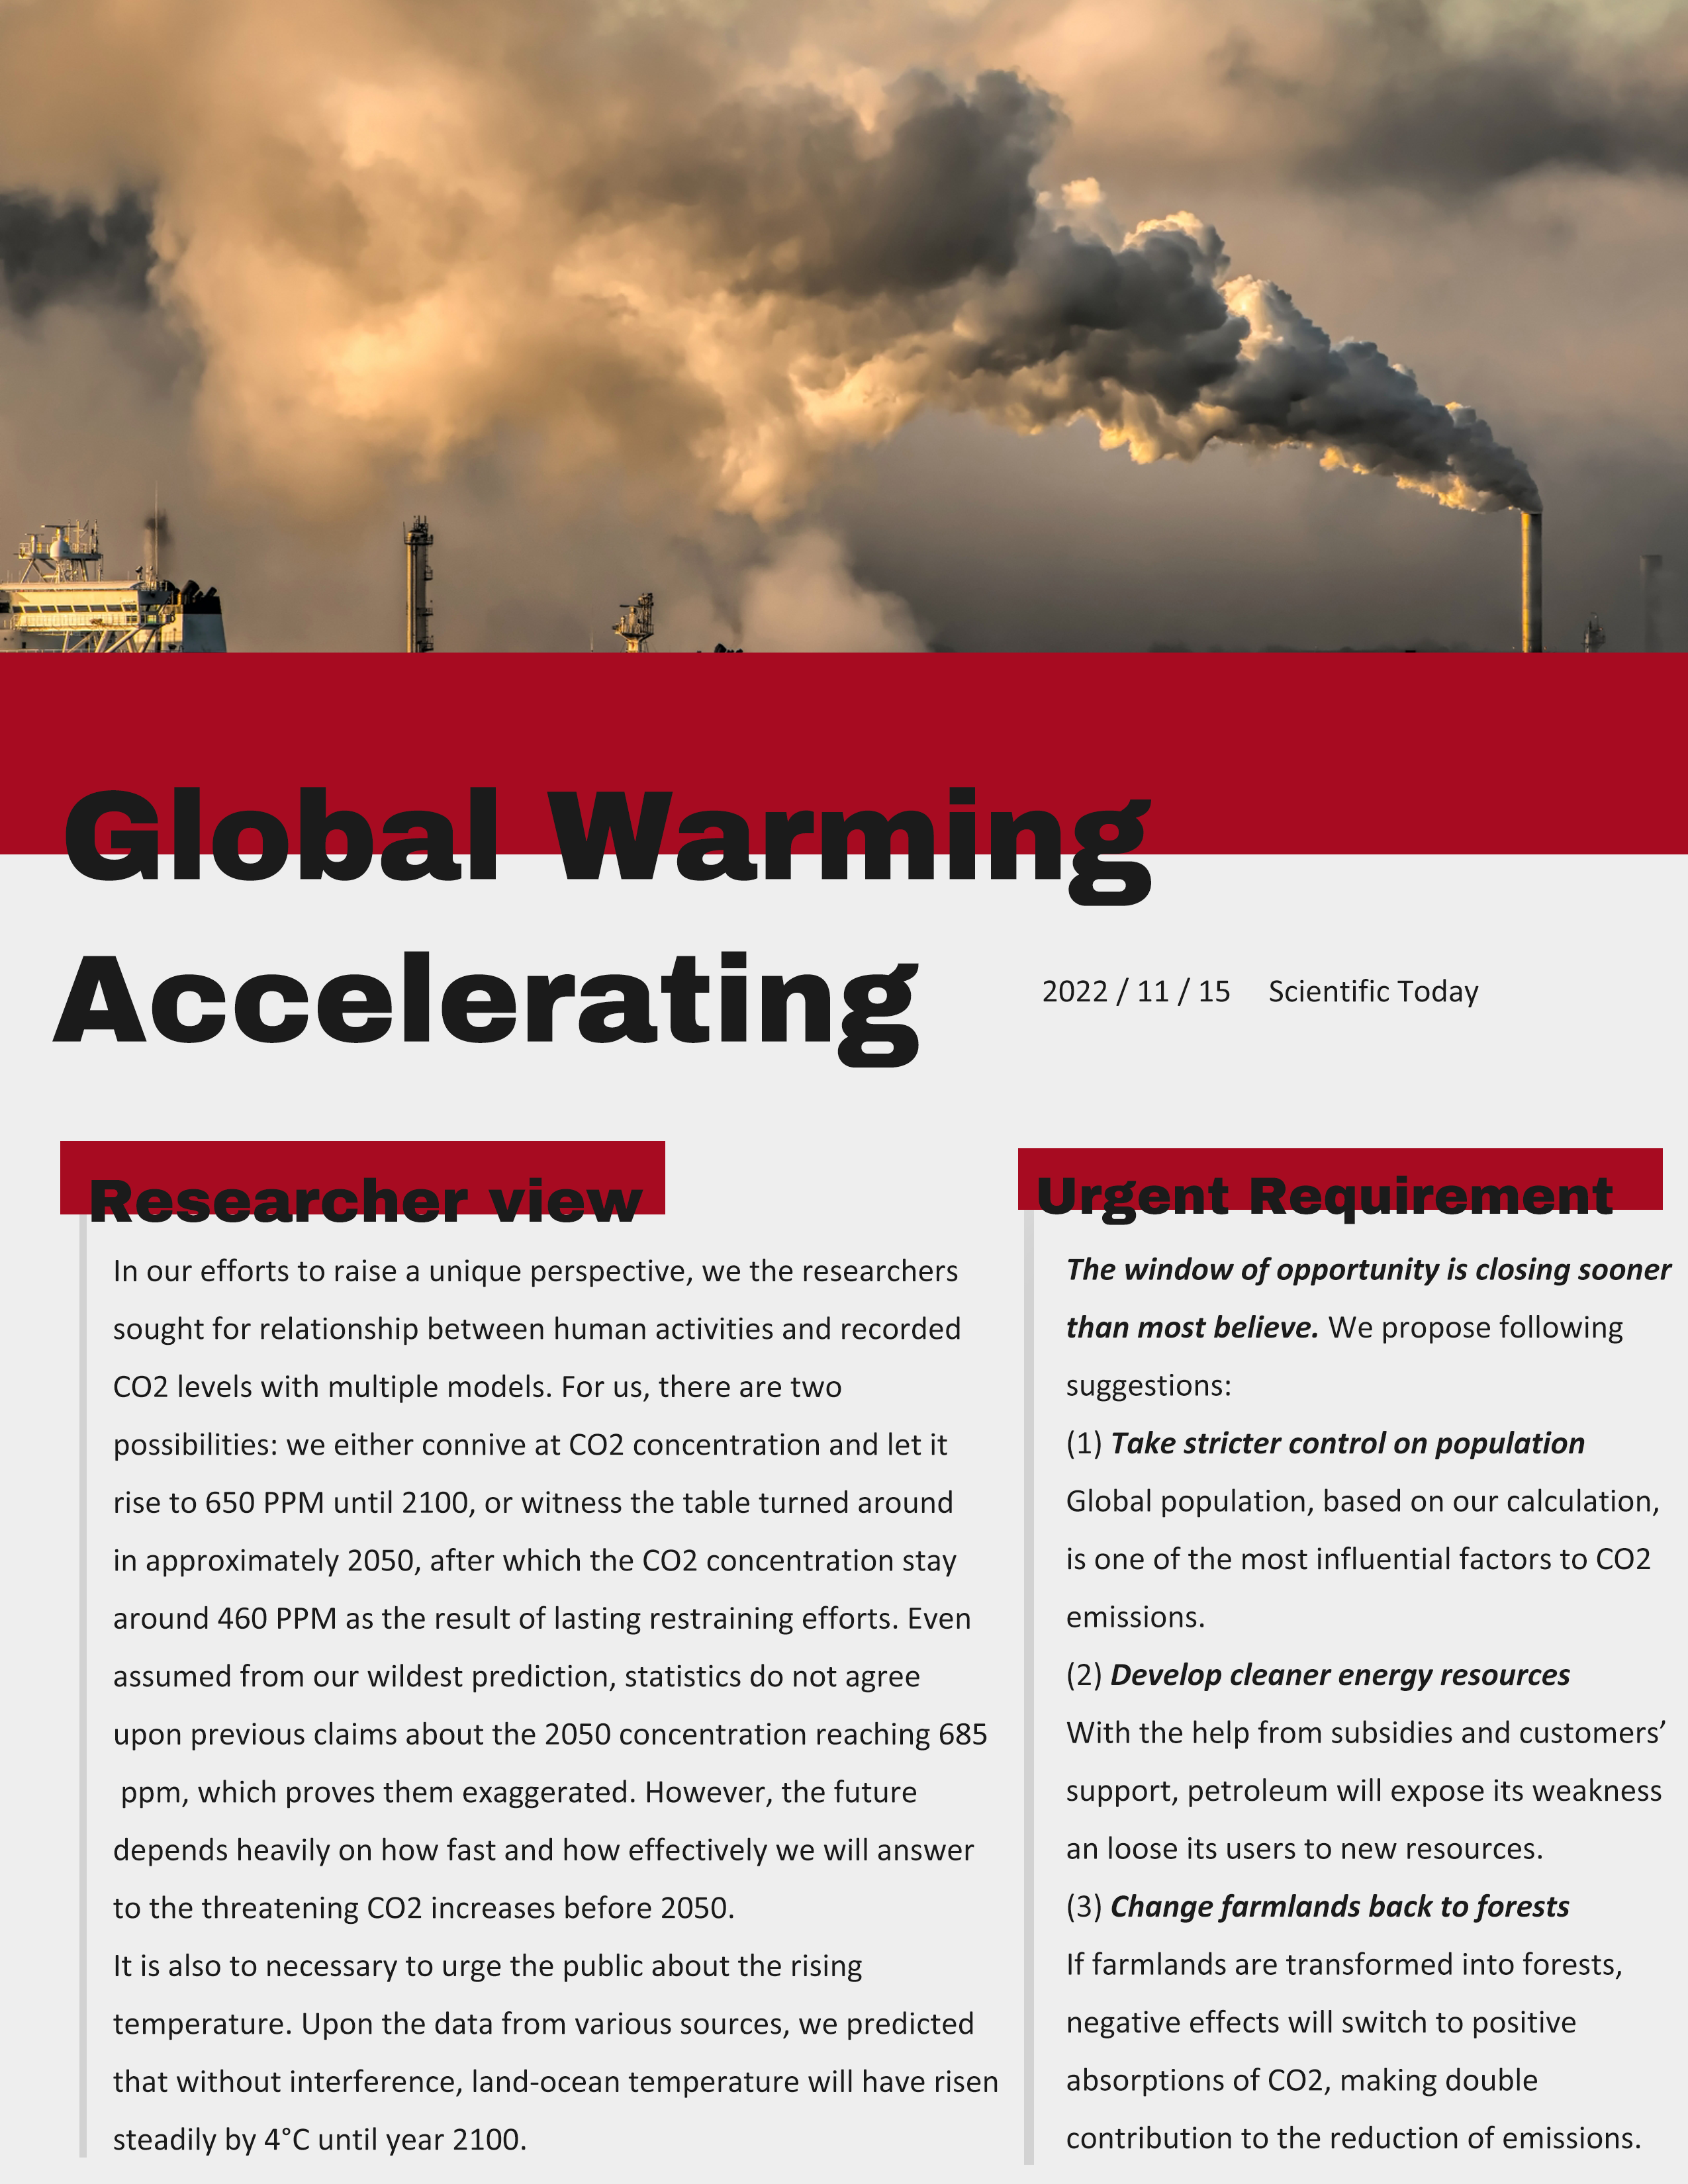
\includepdf[width=\paperwidth]{fig/non-tech.png}
    \end{center}
\end{figure}


\newpage
\thispagestyle{empty}

\begin{spacing}{0.1}
    \tableofcontents
\end{spacing}

\newpage

\section{Problem Background}

From around 800,000 years ago, \ce{CO2} concentration in the atmosphere has stayed relatively stable around 280 parts per million until the Industrial Revolution . From the prevalence of steam engines in the early 19th century and following dazzling evolvement of coal-consuming industries, together with multiple chain effects in economy, has led to rapid increase in \ce{CO2} levels in the atmosphere. The growth rate has kept rocketing with progresses in productivity throughout major industrial renovations. With an annual increase of 2.66 PPM in 2021 -- the tenth consecutive year of an increase over 2 PPM , we are currently facing the highest speed of \ce{CO2} concentrating around the globe since the very beginning of human kind. Yet, not until the last century did modern observations of climate change and global warming remind researchers of the impacts of \ce{CO2} levels worldwide. We are urged to analyze the relevance between \ce{CO2} concentration and temperature to predict future trends for references in environmental conservation, policy making and more sustainable development approaches. 

Factors leading to \ce{CO2} emissions are far beyond estimation, and they are still expanding with new industries emerging from traditional ones. Direct emissions from industrial production and transportation block indirect agricultural factors responsible for increases in \ce{CO2} levels. Apart from the first and the second industry, following economic effects spread across the third industry. In underdeveloped regions, urban populations are booming and taking over more naturally vegetated fields and farmlands, decreasing the \ce{CO2} recycled through photosynthesis. Yet in contrast, the governments in developed regions are proposing carbon neutralization that has already been mentioned in legal reforms and policy making, limiting the rise of \ce{CO2} emissions to various extents. 

These phenomena partially explain the controversy stirred up by predictions about the levels of \ce{CO2} in the atmosphere. In order to stress the urgent need, apart from seeking determining factors for prediction, observations on major variations that close resemble the changes are highly expected. Among these factors, temperature is widely endowed with the most importance, as excessive \ce{CO2} form barriers that block the exit of solar heat that accumulates to arouse greenhouse effects.

\section{Restatement of Questions}

\paragraph{Problem 1:} In order to reassess current claims about \ce{CO2} levels, we will take various factors into account as materials for further modeling. For the creditability of the factors, we should research in advance and filtrate the wide range of emission sources according to relevance, comprehensiveness and reliability. We should then build mathematical models to each of these variations and produce multiple algorithms developed through separated methods. They are expected to describes the historical levels of \ce{CO2} in the atmosphere as early as recorded, so as to predict future changes in \ce{CO2} concentration. It is necessary to mention that despite the general trend of increase in \ce{CO2} emission, efforts made to neutralize the emission across the previous three stages ought not to be forgotten. According to the results, we will come to an opinion for or against the \ce{CO2} level claims and point out exactly when \ce{CO2} concentration reaches 685 PPM.

\paragraph{Problem 2:} To find out the relationship between temperature \ce{CO2} concentration in the atmosphere, we will first need to combine different functions to build a fitting curve for the history of land-ocean temperatures. Upon finishing this section, we will then broaden our scope of analysis to list preselected possible factors influencing global temperature, including \ce{CO2} concentration that we have figured out. Through mathematical processes that inputs historical and predicted concentration, each factor's proportional relative correlation with temperature will then be output to determine if \ce{CO2} is responsible for the majority of rise in temperature. Yet, this process only compares different factors. To acquire the relationship between solely \ce{CO2} and temperature, we need to process previous data outputs of the two variables through a quantifying approach. Results from the comparison, enhanced by a specifically quantified relationship, will support us to answer the problem. 

\section{Assumptions and Justifications}
To simplify the problem, several assumptions and justifications are listed below.

\paragraph{Assumption 1:} Solar Cycle Length maintains stable before 2100 when the prediction ends.

\noindent\textbf{Justification:} As the sun directly radiates a daily 340 watts in forms of heat to each square meter on earth , global temperature is directly connected to the sun's status over long periods of time. Yet its influence on modern changes in global temperature is calculated to be of little importance, and the 11-year length of a single cycle stays basically unchanged over the past century. Yet, the cycle is still viable, occasionally extending the peak or the trough of a cycle. Considering the disparate scale of the heat emitted by the sun and that received by earth, any vibration in the cycle will lead to sudden and drastic changes to temperature. We ought to keep this factor as irrelevant to lower unpredictability. 


\paragraph{Assumption 2:} Catastrophes with global influences, including alien invasion, world wars and large-scale natural disasters, are excluded from determining factors.

\noindent\textbf{Justification:} Upon reflecting on history, it is obvious that sudden turning points are generally out of expectation. Hardly are sudden changes dealt with well or in time, which leads to unpredictable chaos. Moreover, major nuclear-armed countries are to be trusted not to start world wars before 2100. Not only is the assumption realistic, but it also contributes to the simplification of models. 

\paragraph{Assumption 3:} \ce{CO2} concentration is in direct proportion to the influence on heat radiation from earth. 

\noindent\textbf{Justifications:} The major approach in which \ce{CO2} concentration affects the changes in temperature is blocking the radiation of heat from earth into space. Because mathematical methods are limited to multiplying the \ce{CO2} curve to get the level that radiation is blocked, when \ce{CO2} changes equally twice in concentration, the depending blockade to radiation should theoretically change in equal amounts. Otherwise, any model that projects the relationship between \ce{CO2} and temperature will doubted as unrealistic.


\section{Notations}

Note: In most cases, we use lowercase letters(e.g. $c$, $t$, $x_2$) for scalars, boldface letters($\boldsymbol{w}$) for vectors, and uppercase letters($M_\text{pca}$) for matrices. For example, $\boldsymbol{w} = [w_1, w_2, w_3]^T$ and $W = [\boldsymbol{w}_{t1}\  \boldsymbol{w}_{t2}\  \cdots\  \boldsymbol{w}_{tN}]$.

\begin{table}[hbt]
\centering
\caption{Notations used in the paper and explanations}
\label{notations}
\begin{tabular}{cc}
	\toprule
	Notation & Explanation \\
	\midrule

	$c$ & \ce{CO2} concentration in the atmosphere by PPM \\
    $t$ & a certain year \\
    $m$ & number of years we consider in the samples \\
    $h$ & land-ocean temperature at a certain time $t$ \\
	$x_i$ & i-th factors mentioned in section \ref{factors} \\
	$\boldsymbol{x}$ & vector consisting of all ten factors' values \\
	$X$ & $10$ by $m$ matrix, each column represent $\boldsymbol{x}$ of one year\\
    $\boldsymbol{w}$ & 3-dimensional vector that PCA extract from $\boldsymbol{x}$ \\
    $W$ & $3$ by $m$ matrix, each column represent $\boldsymbol{w}$ of one year \\
    $M_{\text{pca}}$ & matrix representing the linear transformation done by PCA \\
    $f_t(t)$ & the human activities feedback function \\
    $f_c(c)$ & the \ce{CO2} concentraion feedback function \\
    $L$ & threshold value for \ce{CO2} concentration feedback \\
    $\exp(x)$ & exponential function $e^x$ \\
    $\bar a$ & arithmetic mean of some vector $\boldsymbol{a}$'s components \\
    $\hat a$ & predicted value of some variable $a$ \\
    $\rho(\boldsymbol{a}, \boldsymbol{b}, \dots)$ & Spearman's coefficient for some vectors \\
    $Cov(\boldsymbol{a}, \boldsymbol{b}, \dots)$ & covariance of some vectors \\

    \bottomrule
\end{tabular}
\end{table}

\section{Methodology: Problem 1}
\label{method:1}

\subsection{Overview}

\begin{figure}[hbt]
    \centering
    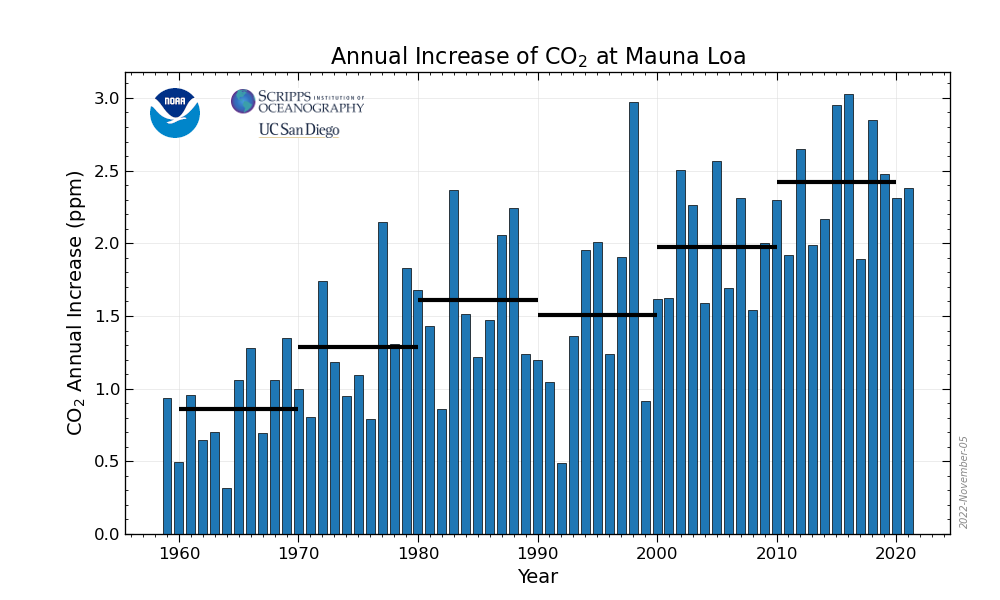
\includegraphics[width = 0.5\textwidth]{fig/co2_data_mlo.png}
    \caption{\ce{CO2} Annual Mean Growth Rate and 10-Year Average Growth Rate}
    \label{p2004}
\end{figure}

Before any models are discussed, we have to make clear that the \ce{CO2} increasing up is never an accident. Figure.1 shows that the 10-year average \ce{CO2} concentraion increase reached a new height in the 2000s. However, this is definitely not caused solely by the 2004 March lift\cite{ref3}.  We can see in the figure clearly that the average tend to increase generally. 

\begin{figure}[hbt]
\centering
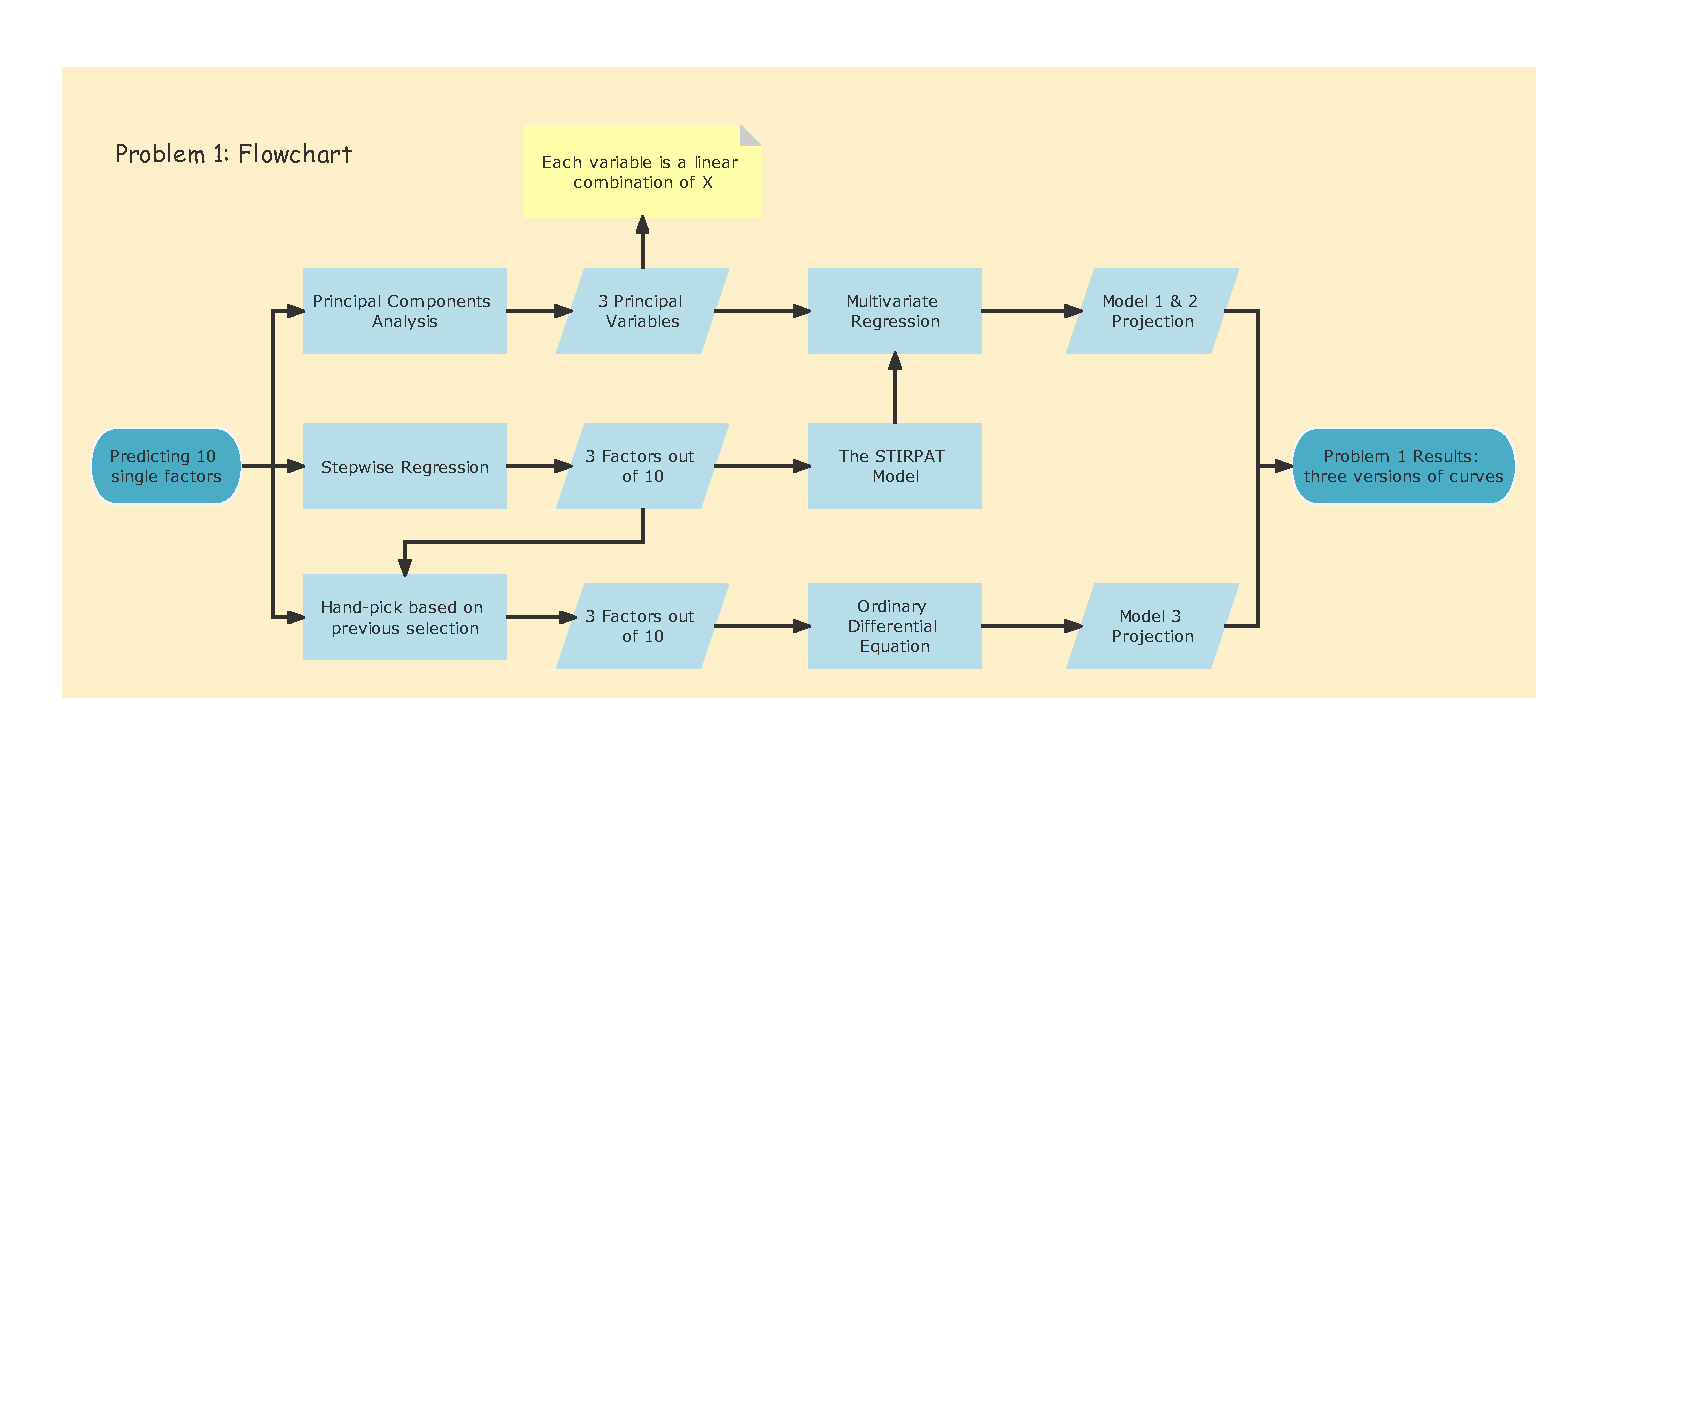
\includegraphics[width = \textwidth]{fig/p1_flowchart.pdf}
\caption{Problem 1 Flowchart}
\label{p1flowchart}
\end{figure}

\paragraph{Aim:} 
Our aim is to build the algorithm that agrees with historical changes and precisely simulate the changes in \ce{CO2} concentration, while taking multiple factors into consideration.

\paragraph{Method:}
We picked 10 major relevant factors, including global population, urban population, GDP, Industry Added Value, Agriculture Added Value, percentage of energy produced from fossil fuel, percentage of energy produced from new resources, GDP per kilogram of petroleum, forest area and farmland area. Based on the records from 1960 to 2021, we fit historical data into ten curves to predict future changes. After evaluating and comparing the weights of the factors, ten curves are then merged into a single curve reflecting future trends of \ce{CO2} levels. We selected three approaches to fit past records most accurately. We made our predictions based on the three curves. 

\subsection{Factor Selection and Projection}
\label{factors}

In order to take the most aspects of influential factors that affects the changes in \ce{CO2} concentration in the atmosphere into consideration, we analyzed statistics released by official institutions available online, for instance the World Bank and the UN Population Division, to identify the data representing the widest range of subordinate fields while avoiding \textbf{overfitting}. Focusing on indirect data influencing from direct \ce{CO2} production helps us extend our vision and avoid wasting time analyzing the sources that had been recorded and summarized previous to our work. For example, urban population represents various \ce{CO2} emitters from human to gasoline, for it uncovers the number of petrol-powered vehicles and thus the amount of gasoline needed. 

We divided selected statistics into three parts: economic data (GDP, Industry Added Value, Agriculture Added Value and GDP per kilo of petroleum), geographical data (global population, city population, forest area and farming area) and sources of energy (energy produced from fossil fuel and energy produced from new resources). 

\subsubsection*{Global Population and Urban Population Projection}

\begin{figure}[hbt]
\centering
    \begin{subfigure}[]{0.4\textwidth}
        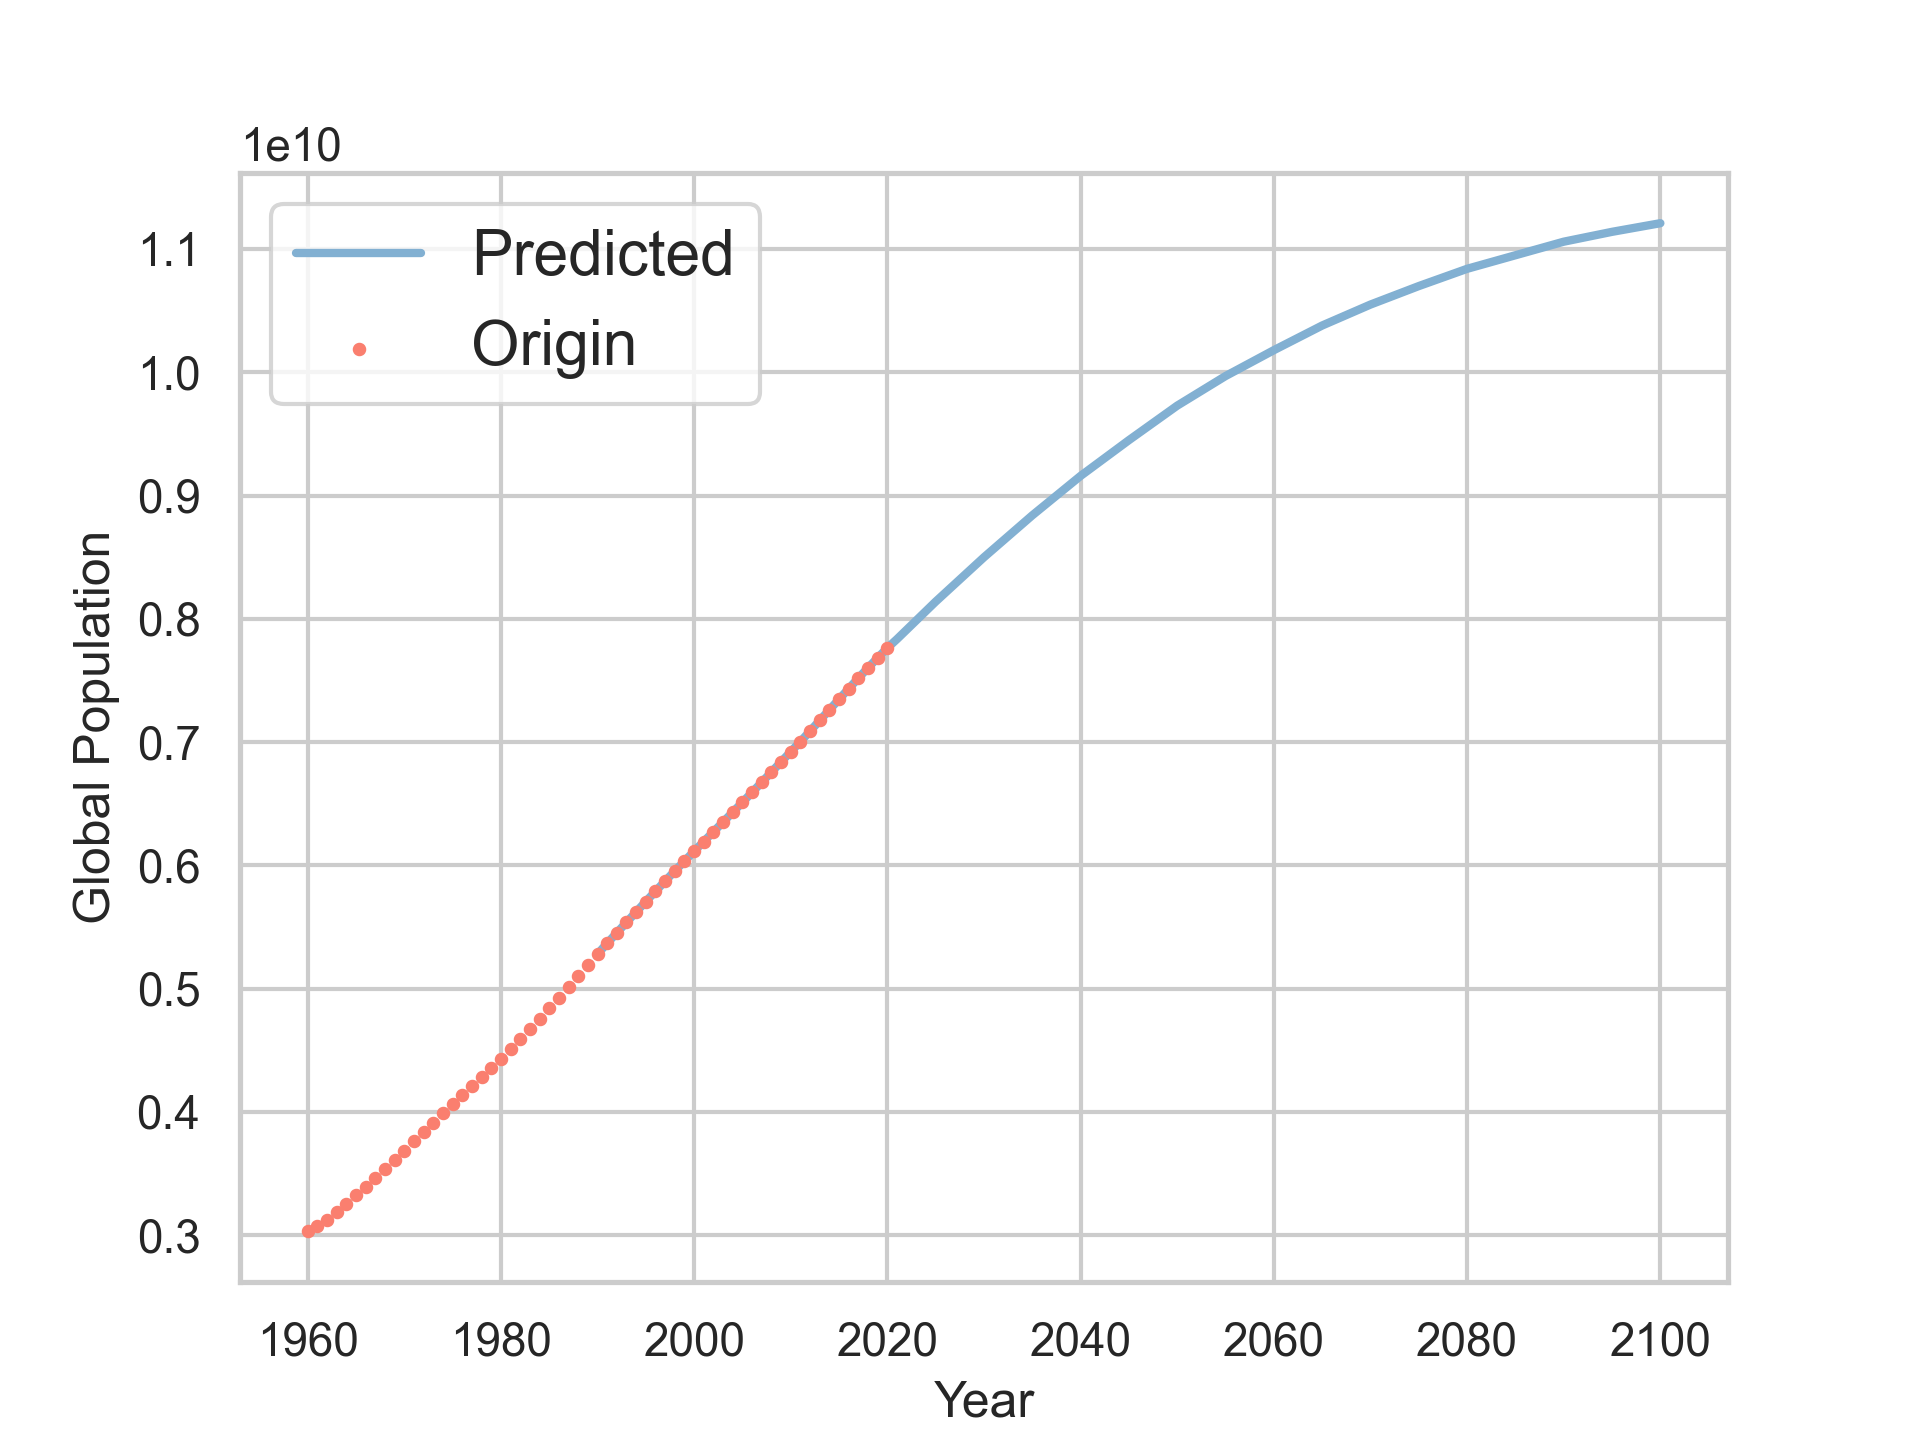
\includegraphics[width = \textwidth]{fig/projection/Global_Population.png}
        \caption{Global Population}
    \end{subfigure}
    \begin{subfigure}[]{0.4\textwidth}
        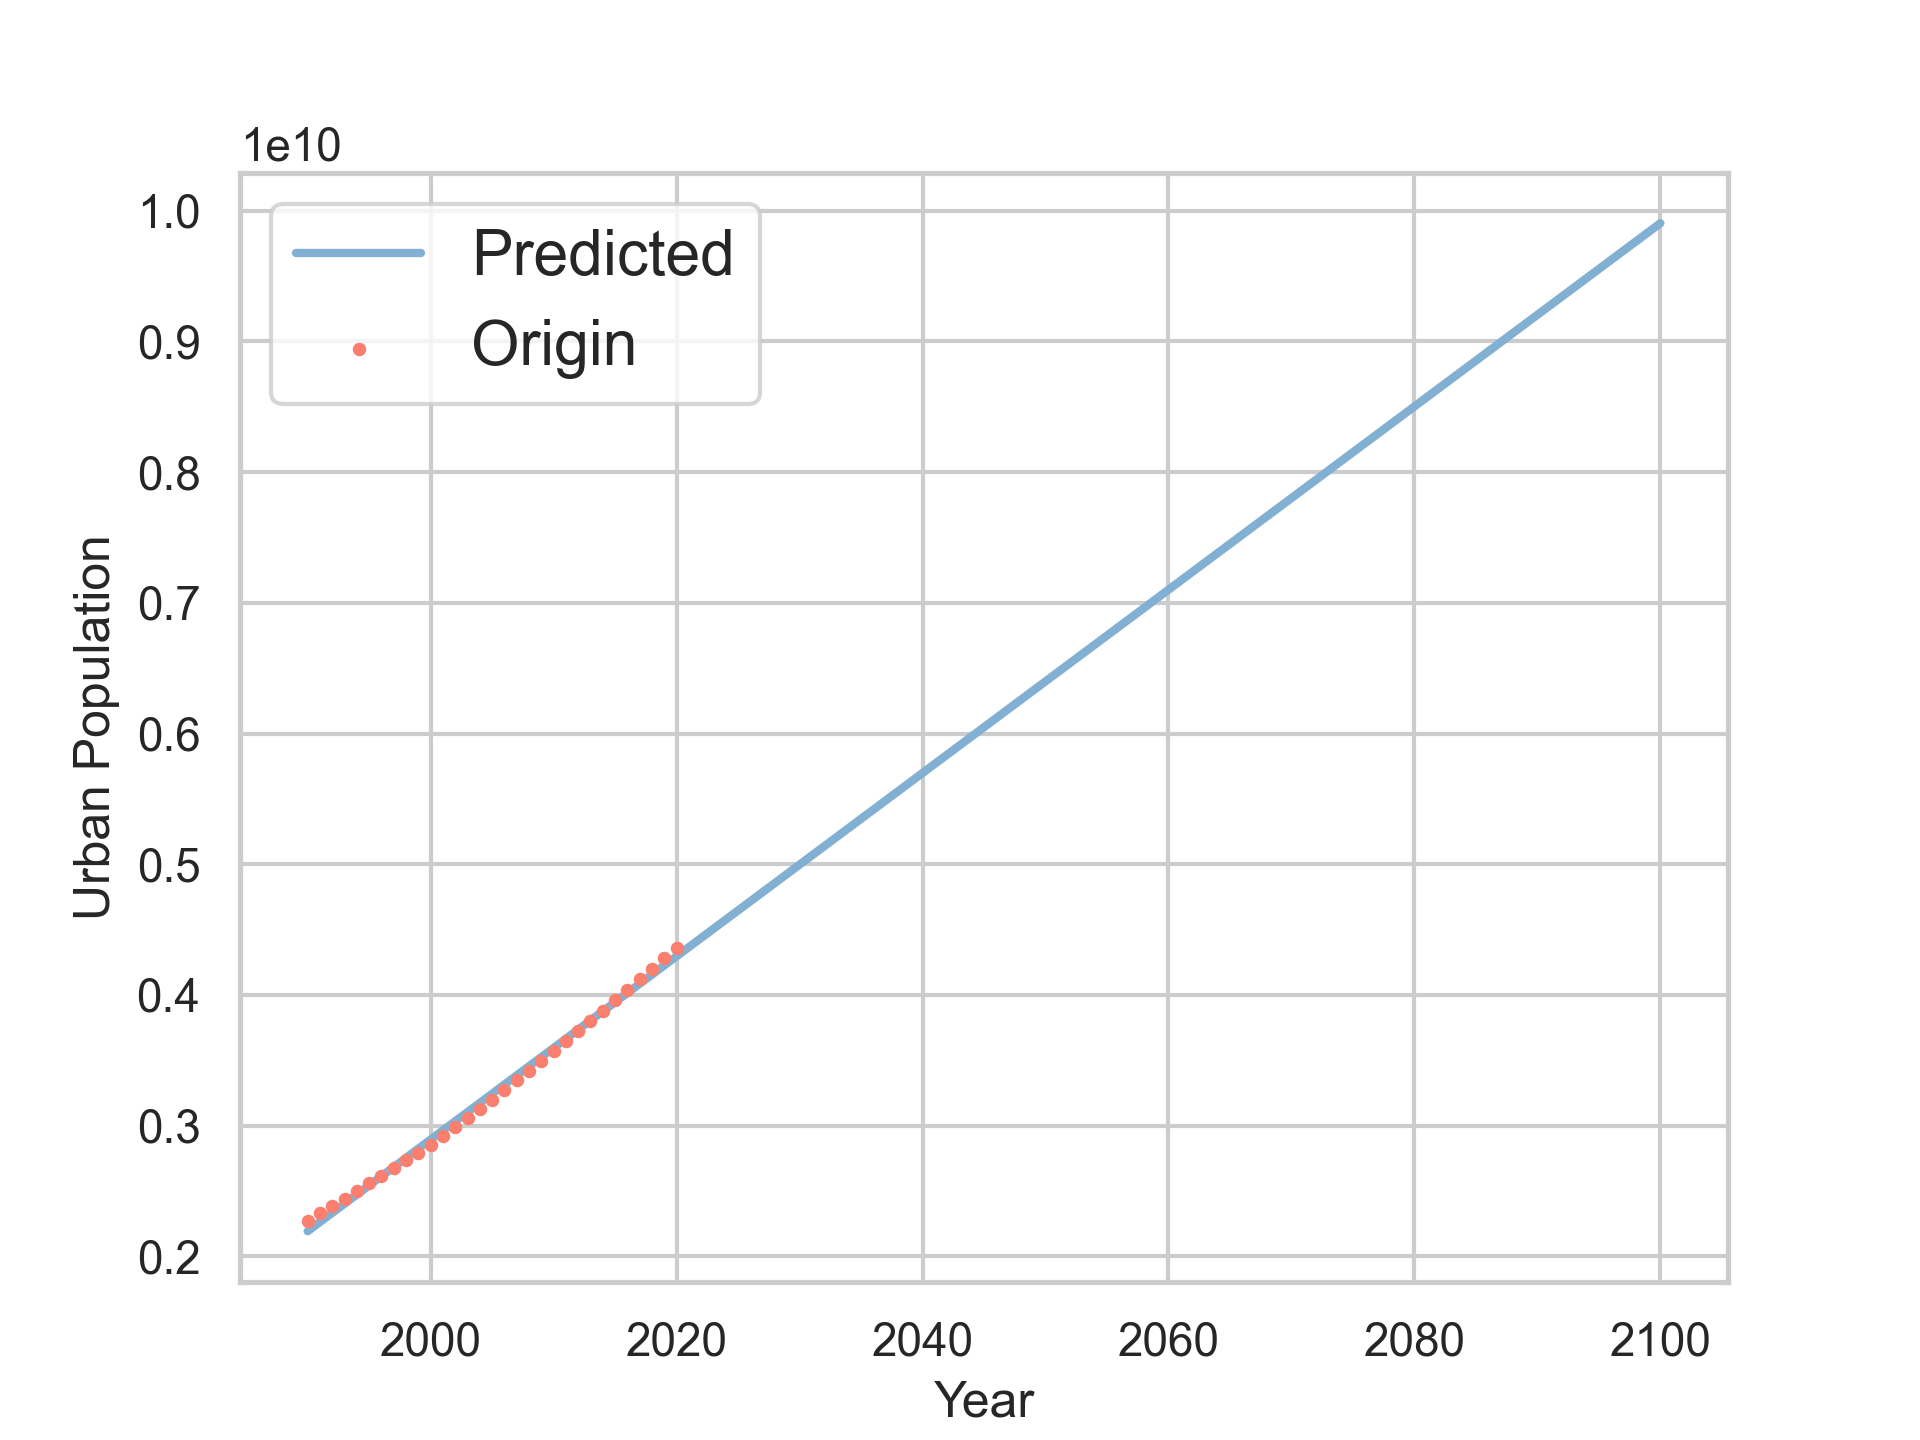
\includegraphics[width = \textwidth]{fig/projection/Urban_Population.png}
        \caption{Urban Population}
    \end{subfigure}
\caption{Predicted Global \& Urban Population}
\end{figure}

Global population, represented by the variable $x_1$, decides the total amount of \ce{CO2} emitted from human breathing and related emissions, including livestock breathing, industrial emissions and transportation emissions. In industrialized regions where the majority of \ce{CO2} emissions other than biological metabolism take place, various sources of \ce{CO2} emission in urban areas, including industrial emissions and wastes from petrol powered vehicles, are affected by the variable urban population $x_2$, because population is directly connected to the size, affluence and ownership of \ce{CO2}-producing machineries. Thus, the total quantum of \ce{CO2} emitted from these resources are represented with relatively high integrity. On global population, we referred to the prediction of the UN Population Division. We predict future urban population with the linear regression model.  

\subsubsection*{Forest Area and Farming Area Projection}

\begin{figure}[hbt]
    \centering
        \begin{subfigure}[]{0.4\textwidth}
            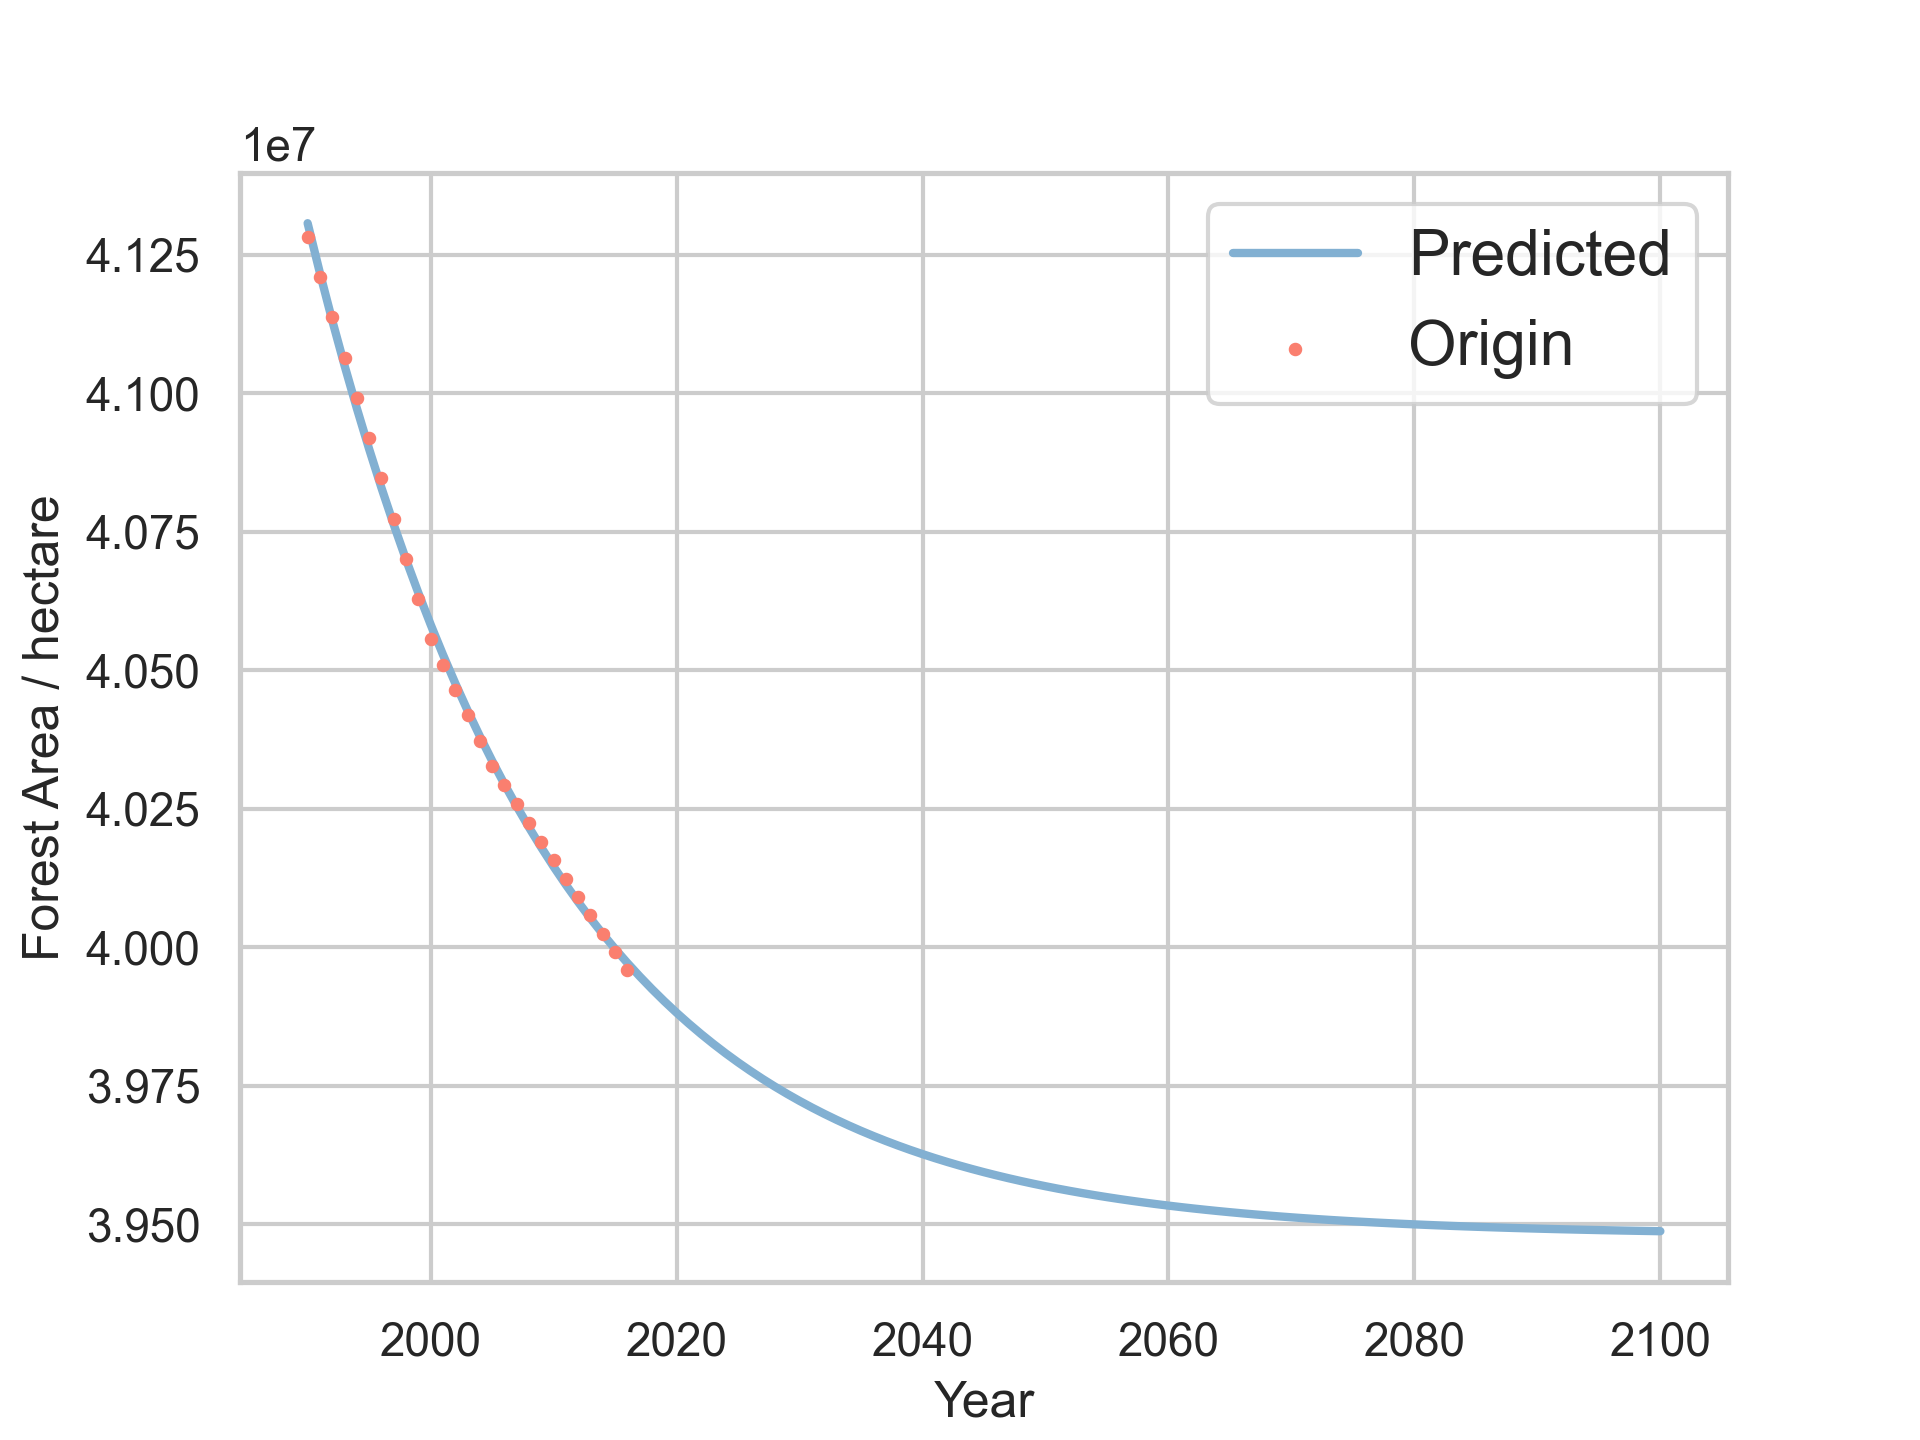
\includegraphics[width = \textwidth]{fig/projection/Forest_Area.png}
            \caption{Forest Area}
        \end{subfigure}
        \begin{subfigure}[]{0.4\textwidth}
            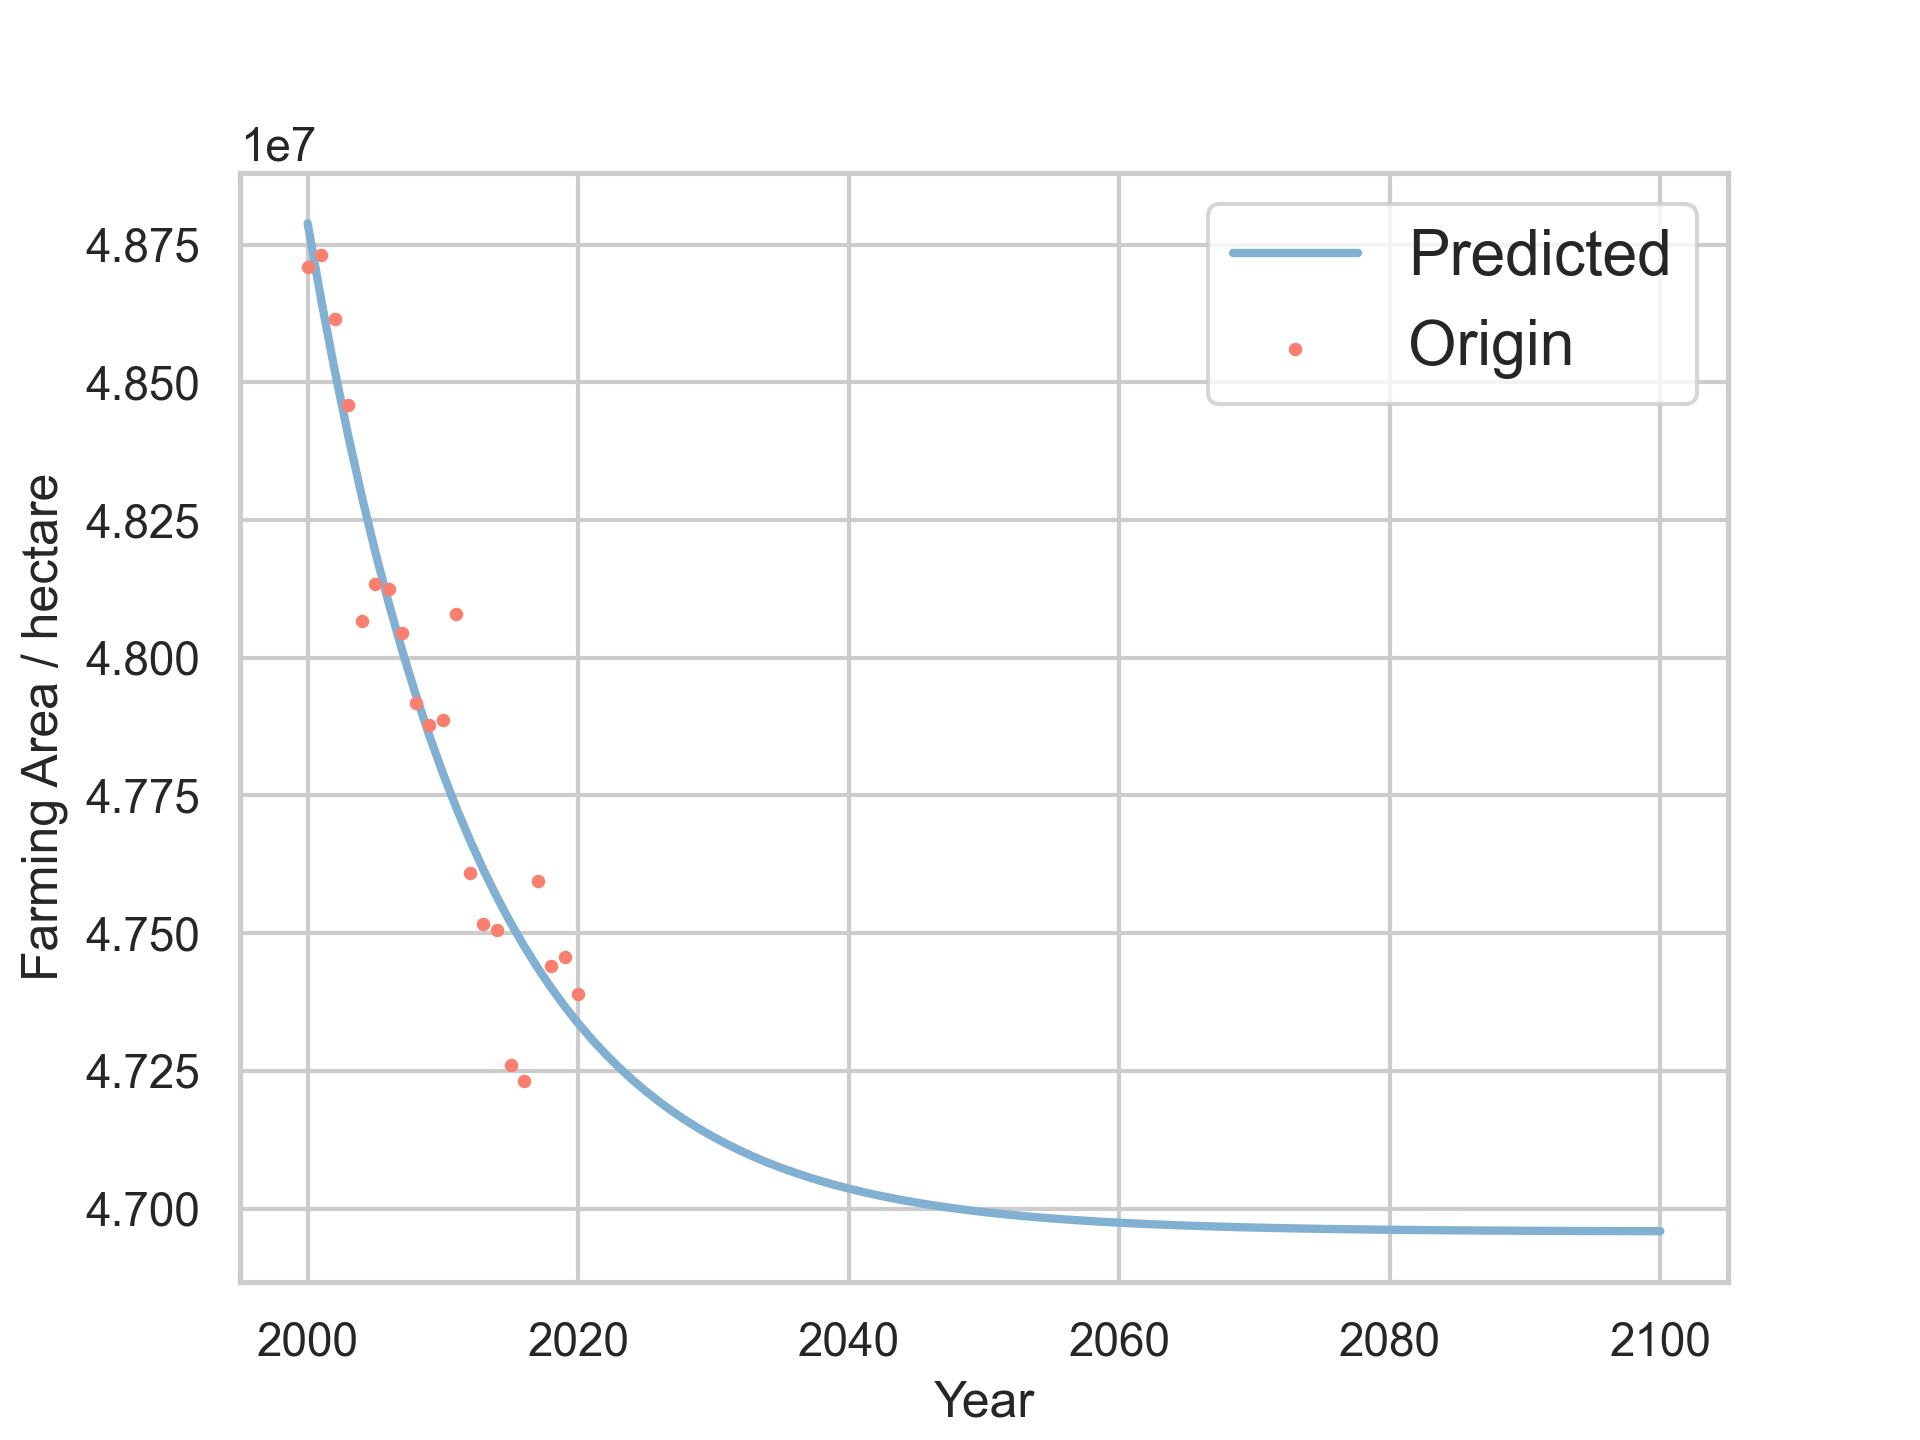
\includegraphics[width = \textwidth]{fig/projection/Farming_Area.png}
            \caption{Farming Area}
        \end{subfigure}
    \caption{Predicted Forest \& Farming Area}
\end{figure}

According to a 2014 NASA report, boreal and tropical forests absorbed a total of 2.5 billion metric tons of carbon dioxide that year. Through photosynthesis, plantations in forest areas contributes more to the absorption of \ce{CO2} concentration in the atmosphere than any artificial or natural approach. Moreover, the vast area that forest covers and high efficiency of photosynthesis produces multiple effect on \ce{CO2} levels. Hence, changes in forest areas play an important role in the reduction of \ce{CO2} in the atmosphere. In contrast, farmlands bear less diversity in plant species, and crops are harvested once they turn ripe. During growing period, plants usually release more \ce{CO2} than they take in. For that chemical fertilizer and harvesters used in farmlands also emit \ce{CO2}, farming areas in fact accelerate the rise of \ce{CO2} concentration.

Based upon the data, we chose \textbf{exponential attenuation} to model of forest and farming areas from year 2000 to 2100. As time passes by, the rates by which forest and farming areas decrease also goes down, which follows the \textbf{exponential attenuation distribution}. Hence, the resulting curves bear close resemblance to reality.


\subsubsection*{GDP, Industry \& Agriculture Added Value Projection}

\begin{figure}[hbt]
    \centering
        \begin{subfigure}[]{0.4\textwidth}
            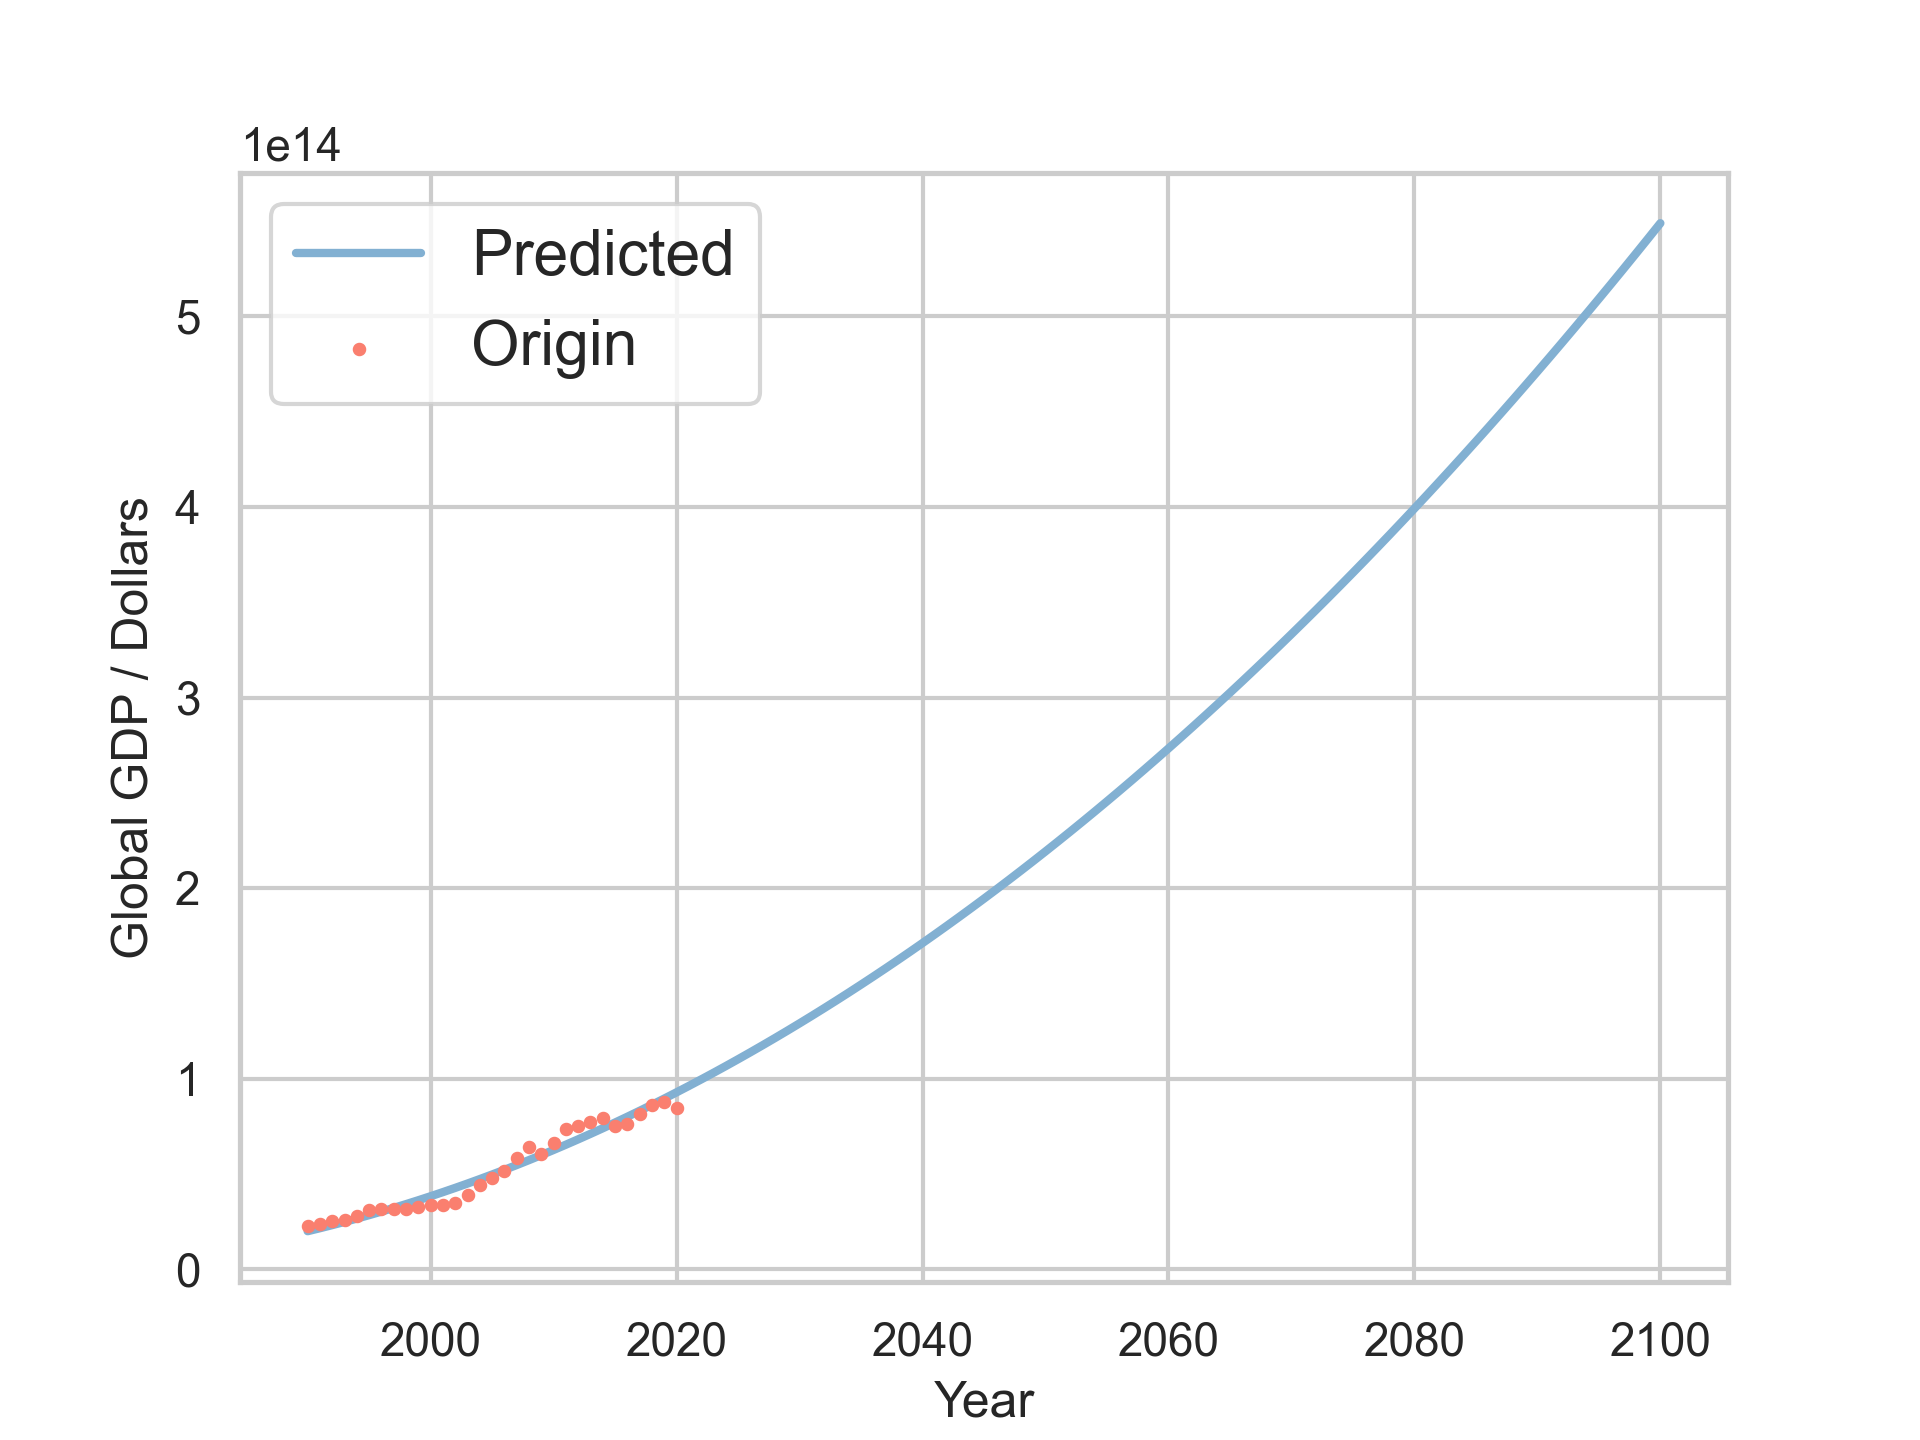
\includegraphics[width = \textwidth]{fig/projection/Global_GDP.png}
            \caption{Global GDP}
        \end{subfigure}
        \begin{subfigure}[]{0.4\textwidth}
            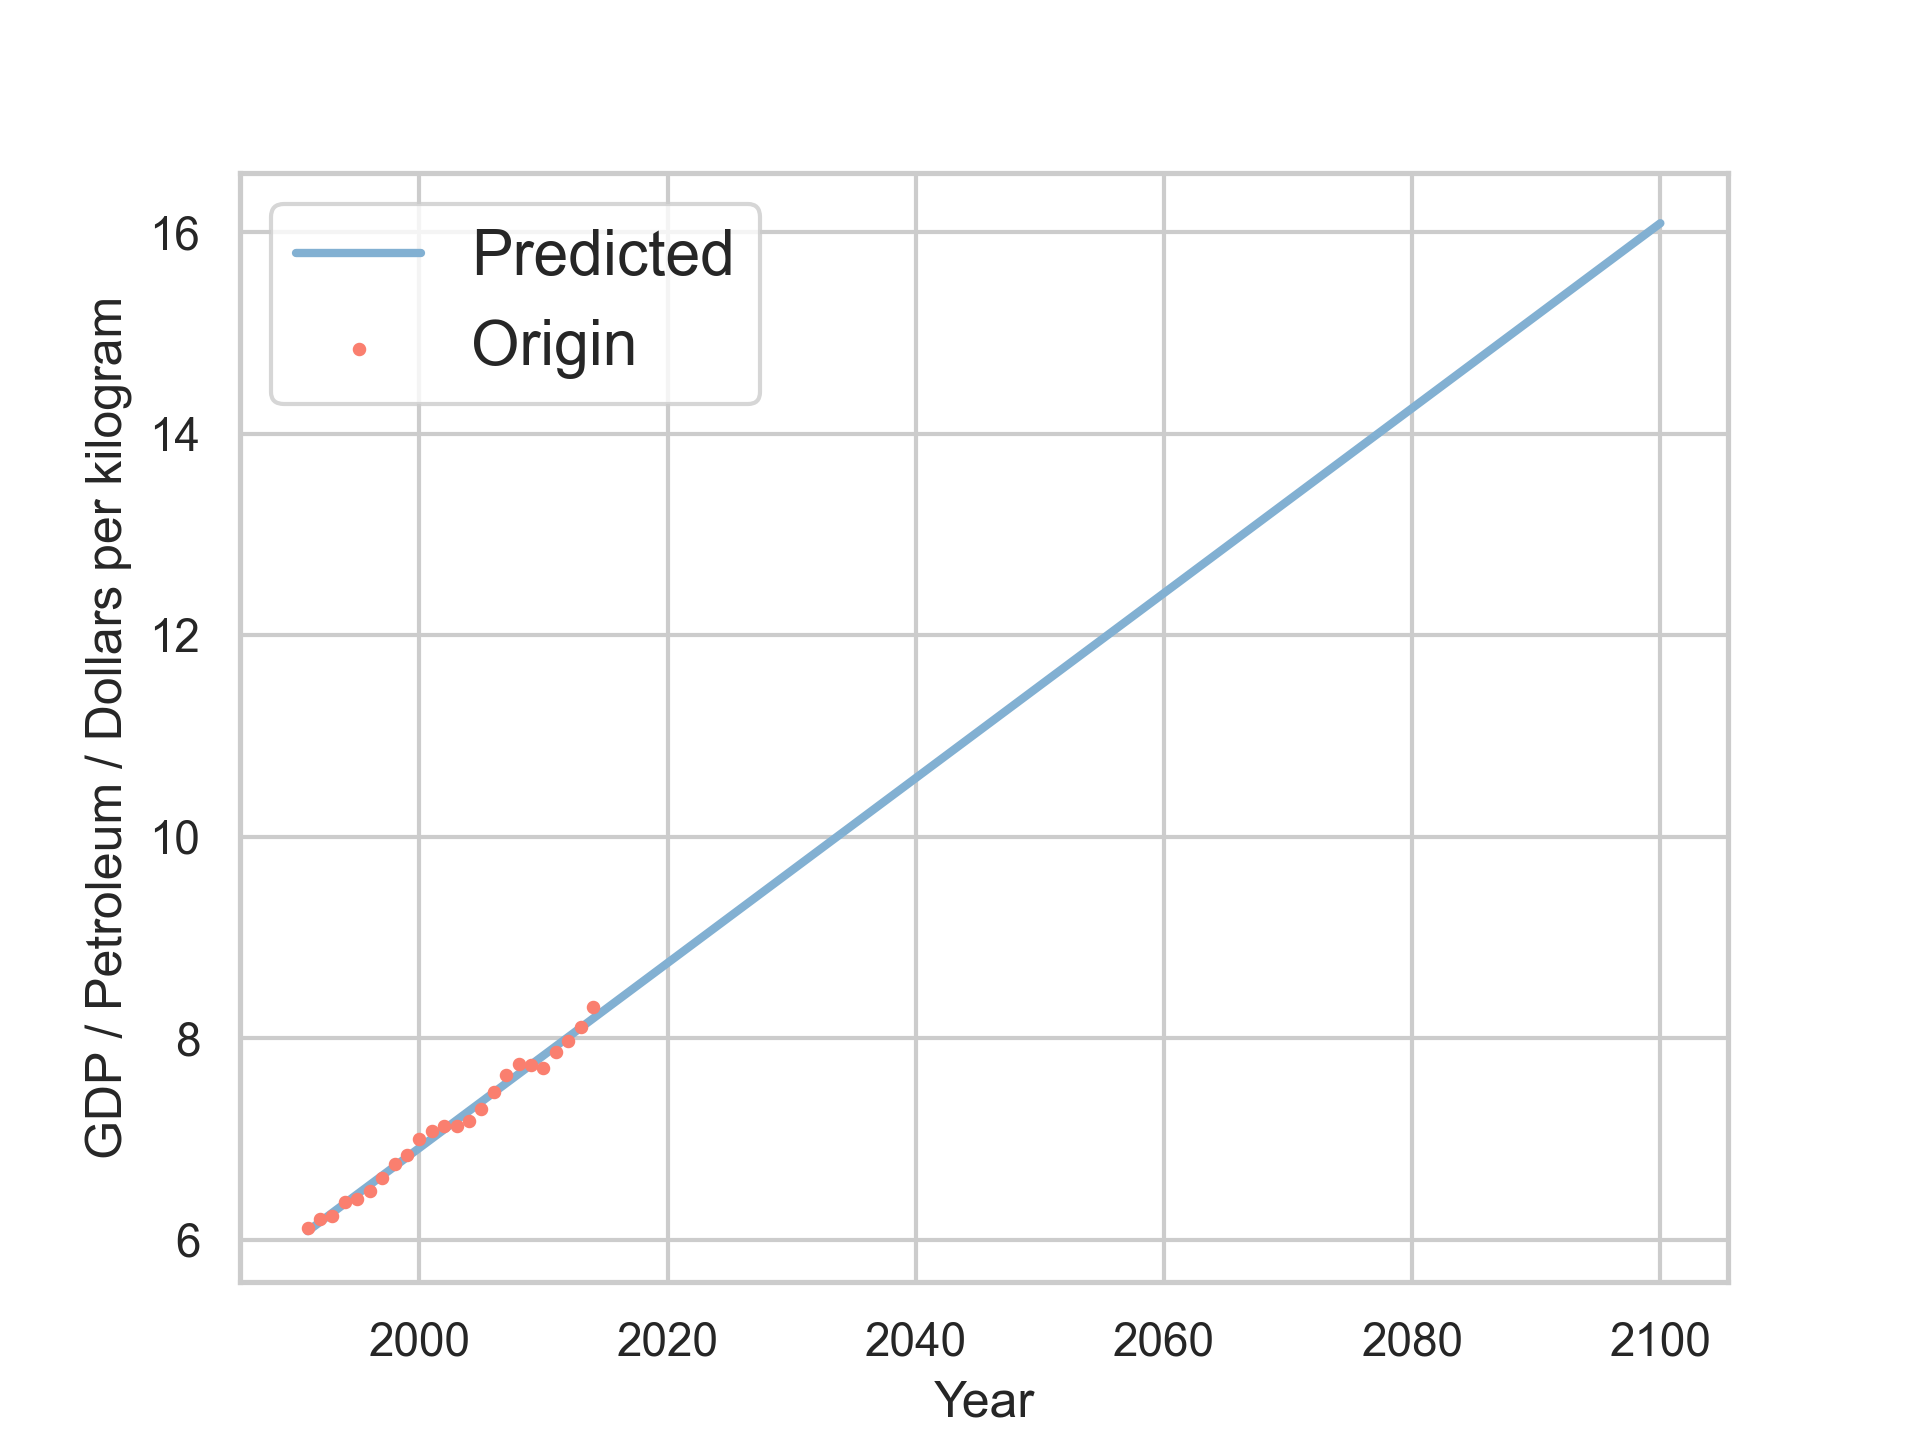
\includegraphics[width = \textwidth]{fig/projection/GDP__Petroleum.png}
            \caption{GDP per Petroleum}
        \end{subfigure}
    \end{figure}
    \begin{figure}[hbt]
        \centering
        \begin{subfigure}[]{0.4\textwidth}
            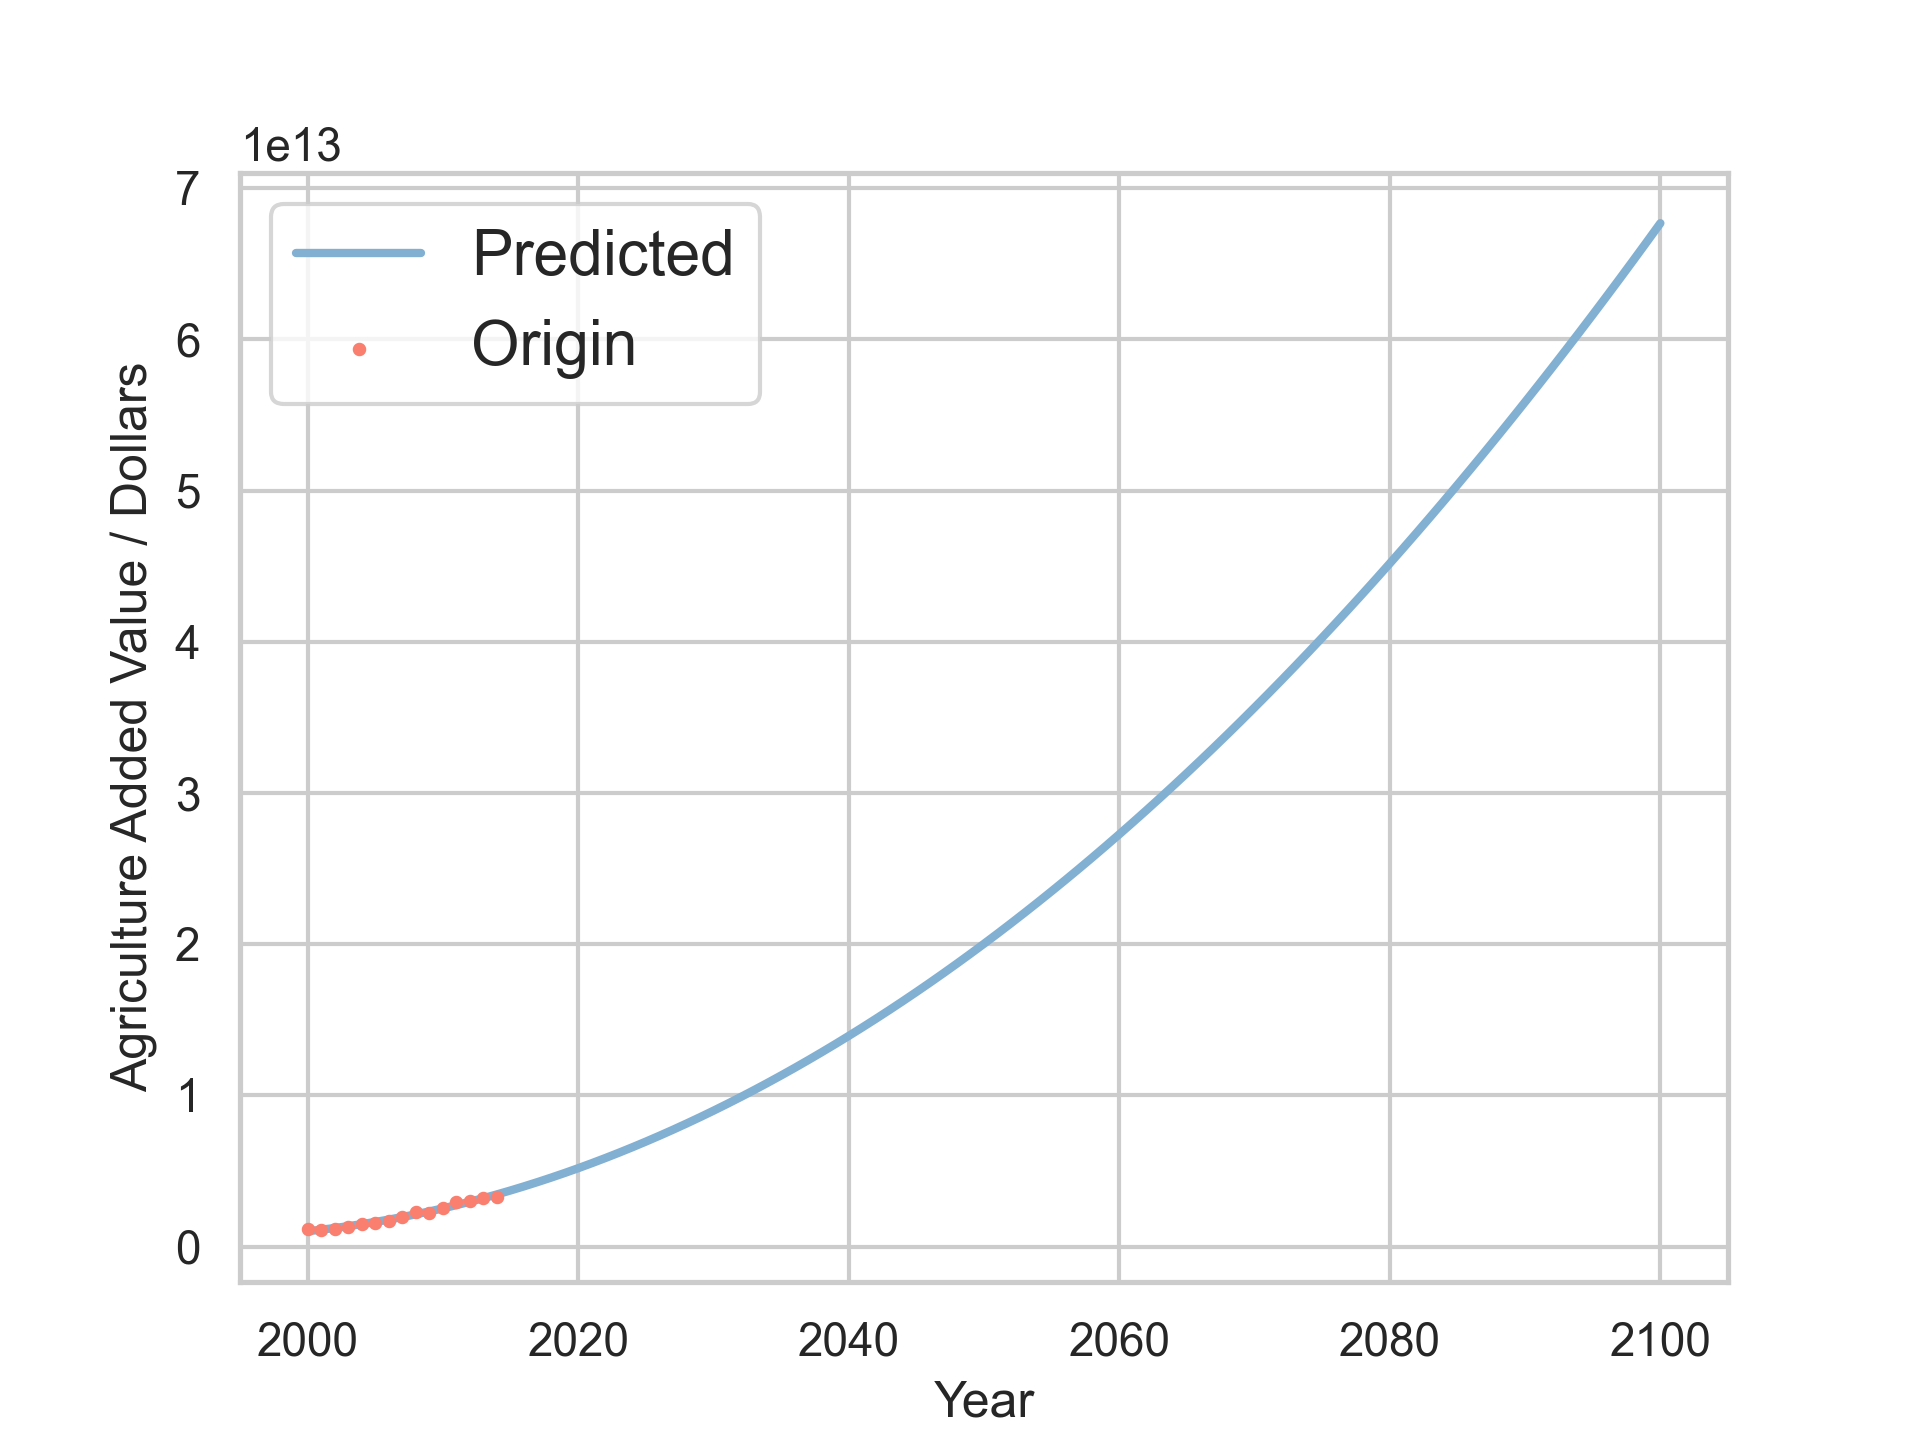
\includegraphics[width = \textwidth]{fig/projection/Agriculture_Added_Value.png}
            \caption{Agriculture Added Value}
        \end{subfigure}
        \begin{subfigure}[]{0.4\textwidth}
            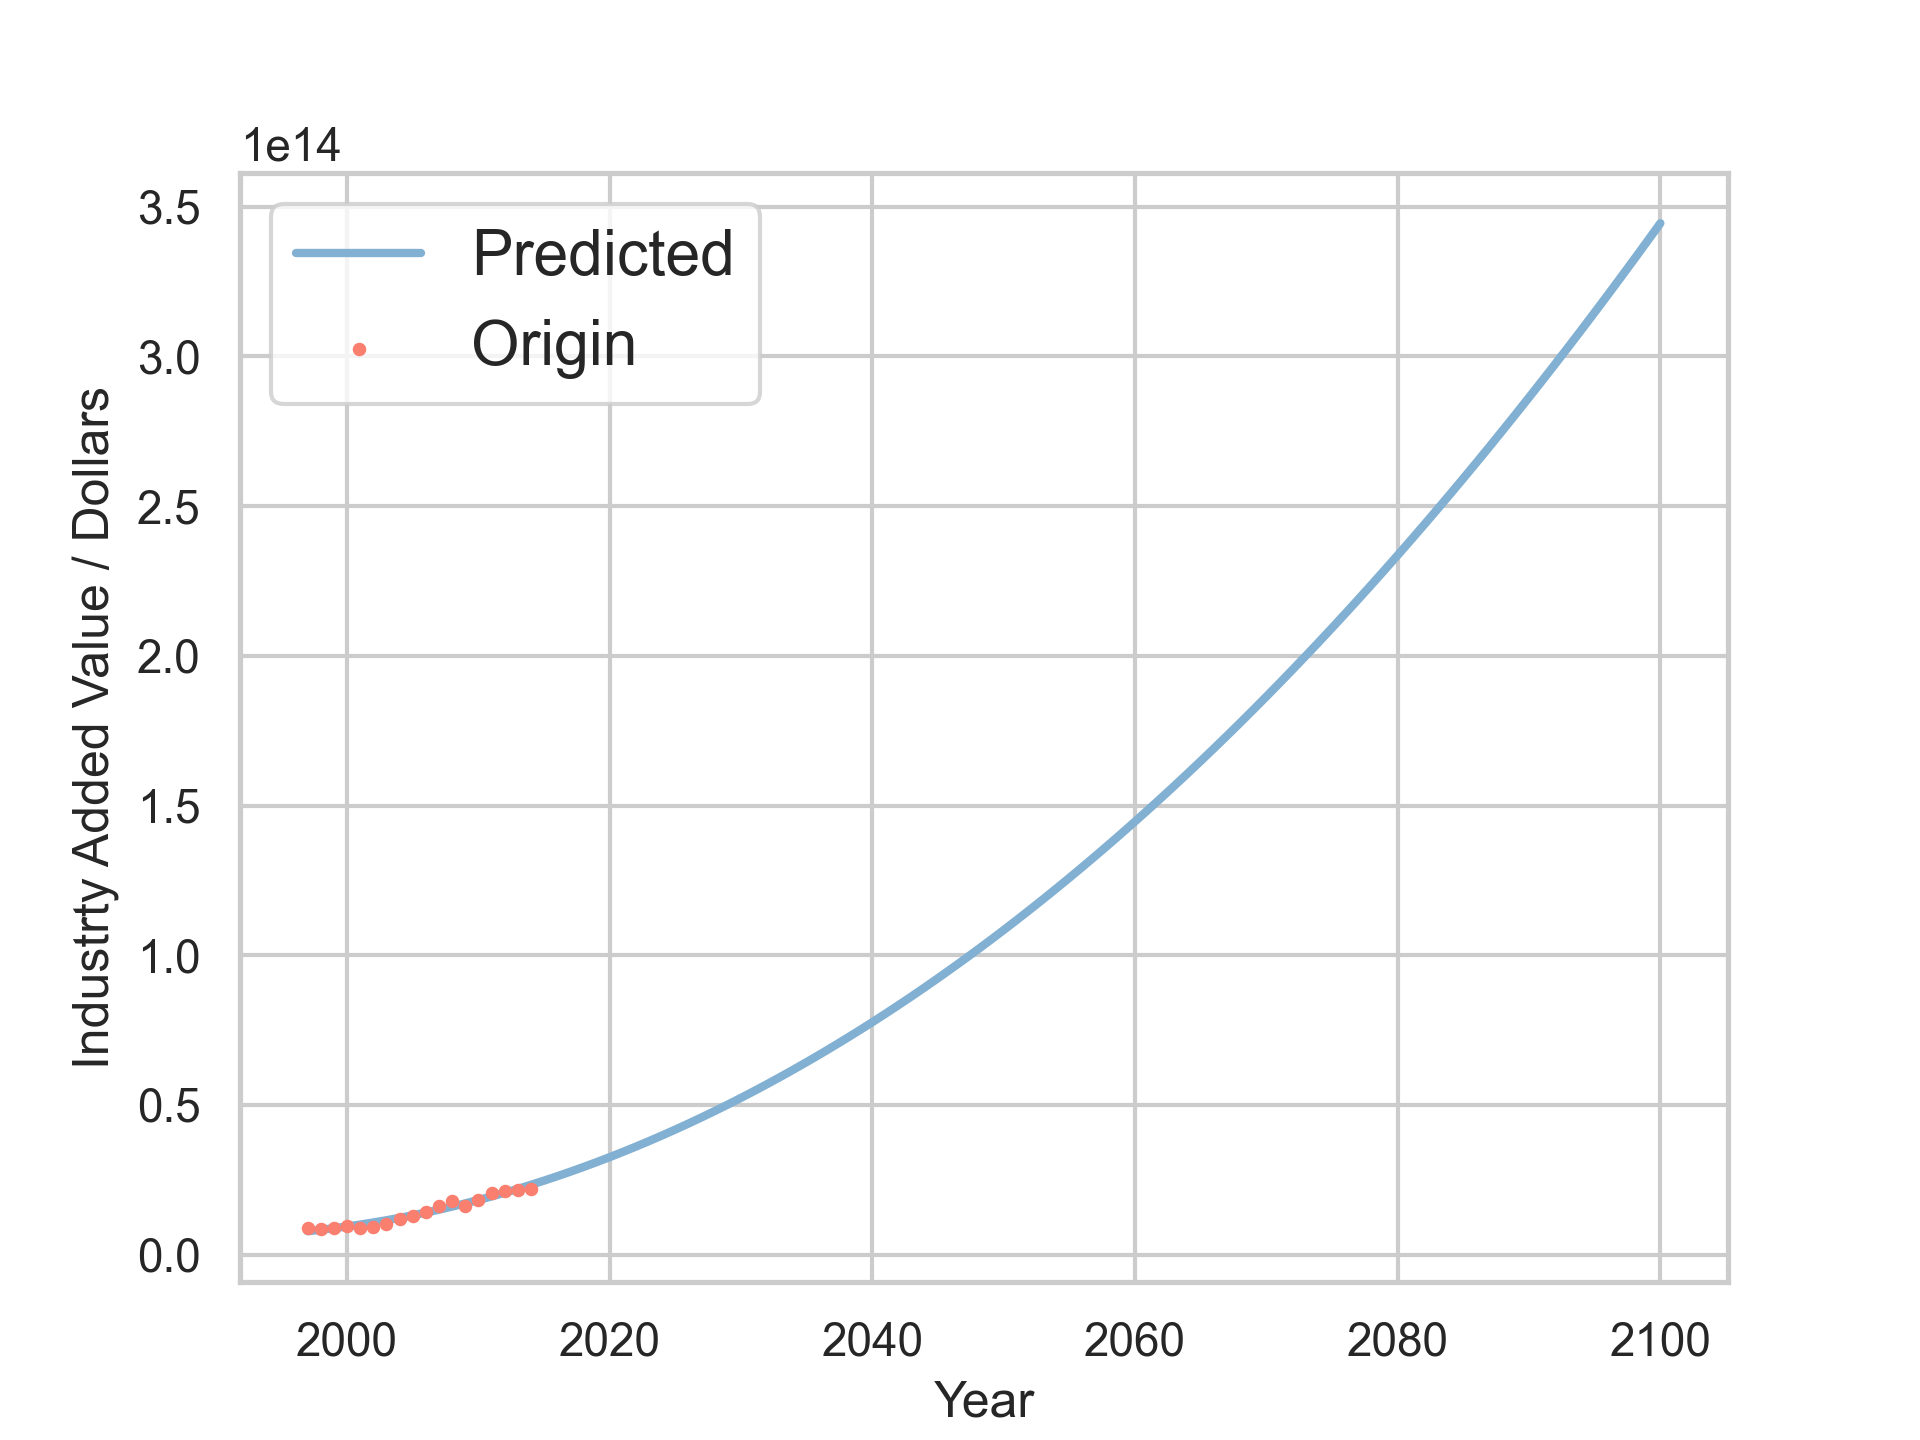
\includegraphics[width = \textwidth]{fig/projection/Industrty_Added_Value.png}
            \caption{Industrial Added Value}
        \end{subfigure}
    \caption{Predicted Economic Factors}
\end{figure}

Originally, involving numerous industrial chains that go across thousands of industries, the wide range of emitting sources are nearly countless. To generate them, we selected four factors to show the frequency and quantity that goods and service are traded across the world, mainly in industrial and agricultural aspects. Behind these trades is \ce{CO2} emissions in production, transportation and utility. By involving these statistics into consideration, we are able to include as much sources of \ce{CO2} as possible, widening the scope of analysis while previous factors provide depth into key aspects. Specially, we chose the value of GDP/petroleum to better visualize the consequent \ce{CO2} levels produced by the processes behind these numbers. 

Despite slight fluctuations from time to time, Global GDP, Industry Added Value, Agricultural Added Value have all been growing with global economy in general until 2022. We used linear and quadratic functions to optimize the calibration accuracy. 


\subsubsection*{Energy Production Projection}

\begin{figure}[hbt]
    \centering
        \begin{subfigure}[]{0.4\textwidth}
            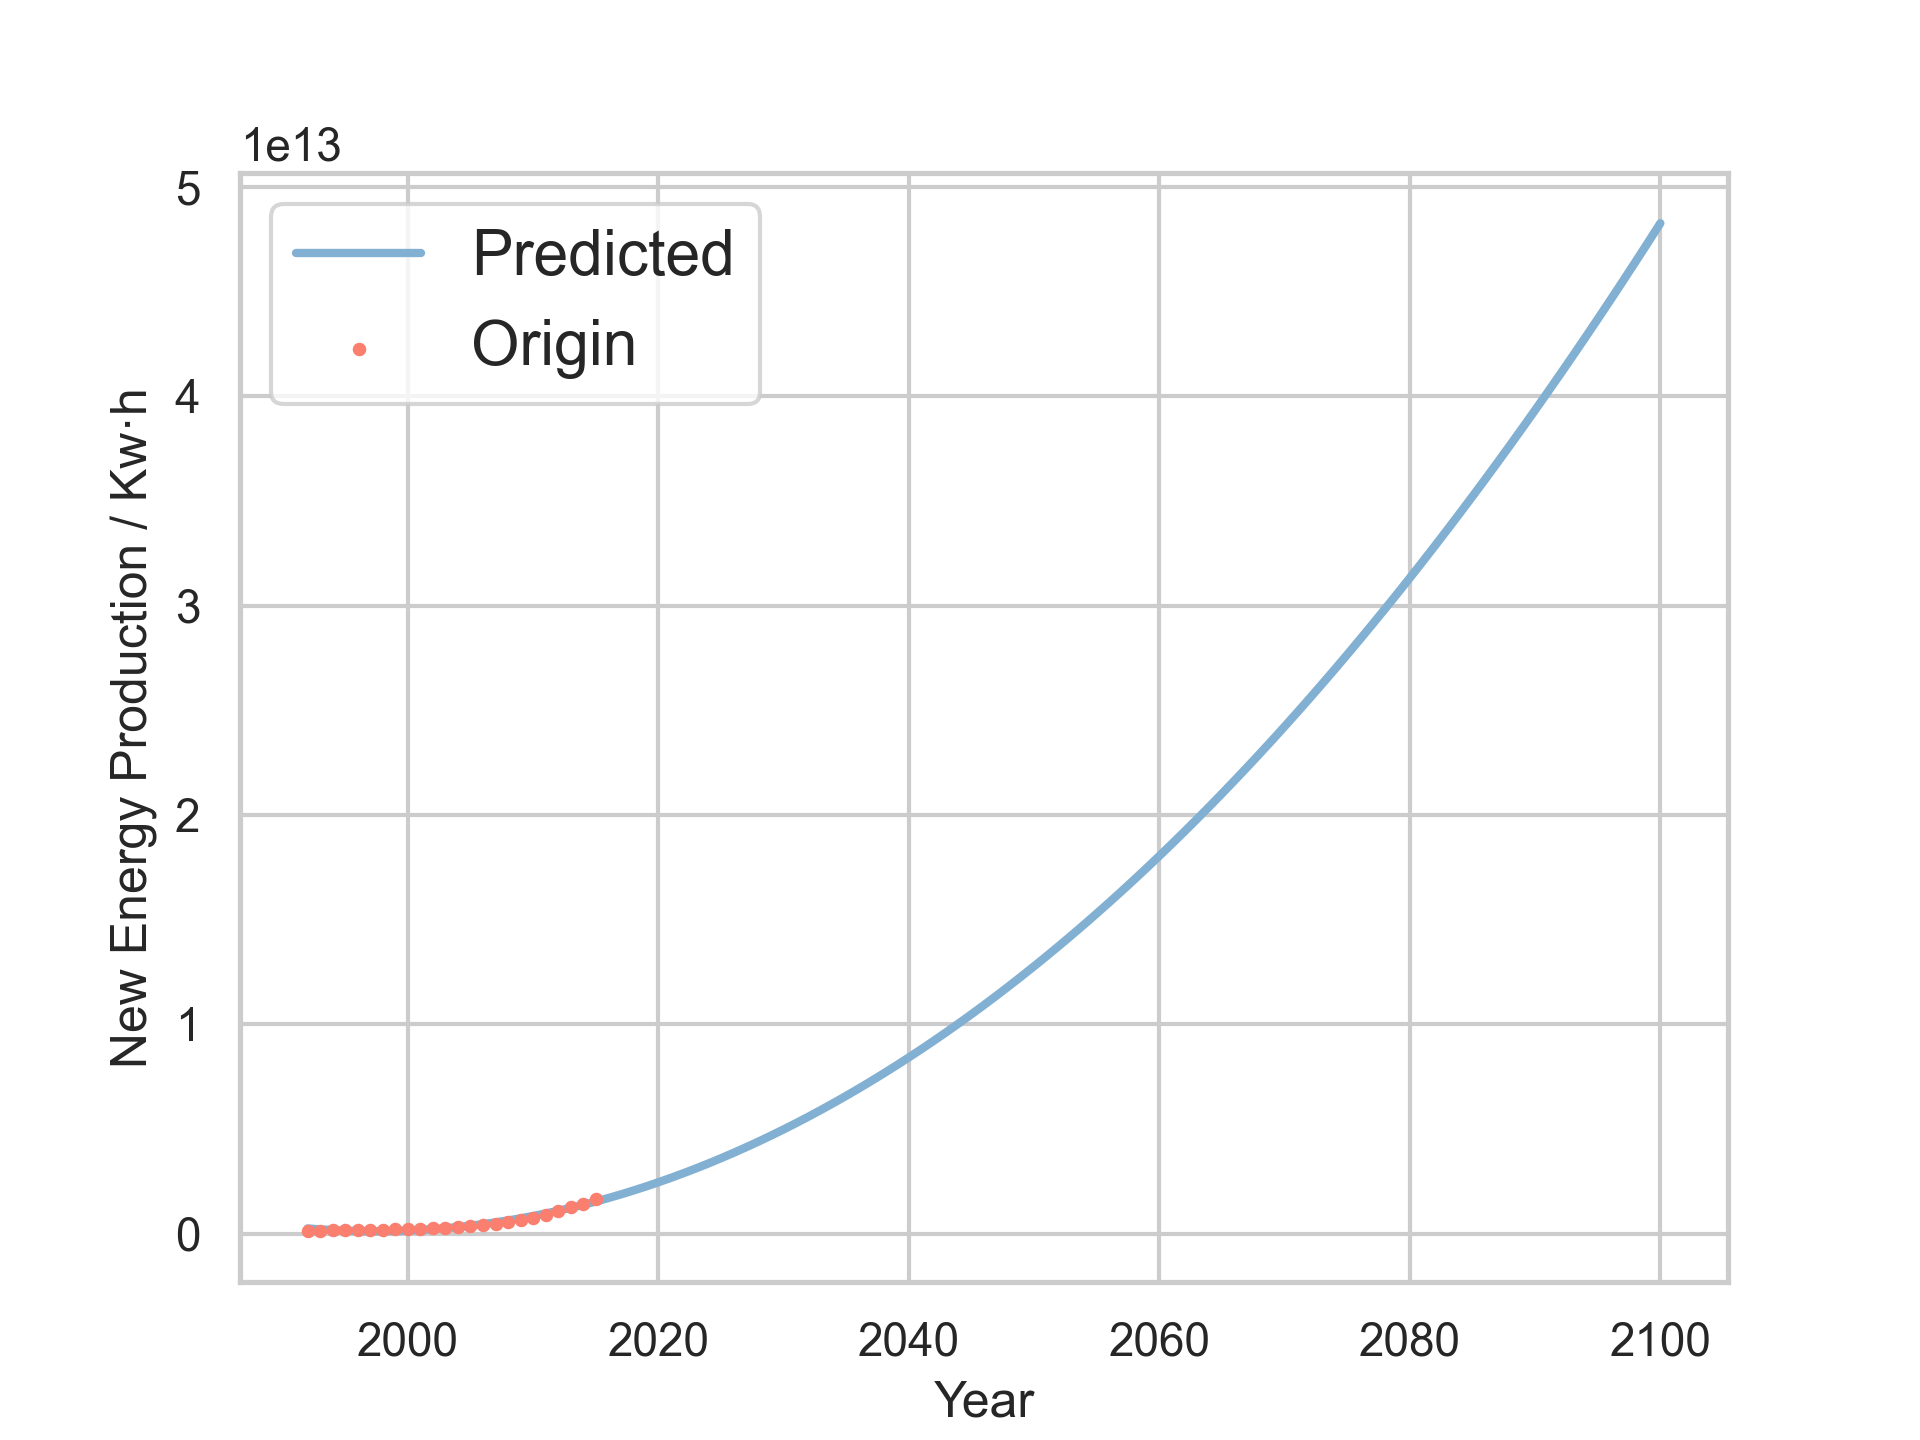
\includegraphics[width = \textwidth]{fig/projection/Energy_Production__New_Energy.png}
            \caption{New Energy Production}
        \end{subfigure}
        \begin{subfigure}[]{0.4\textwidth}
            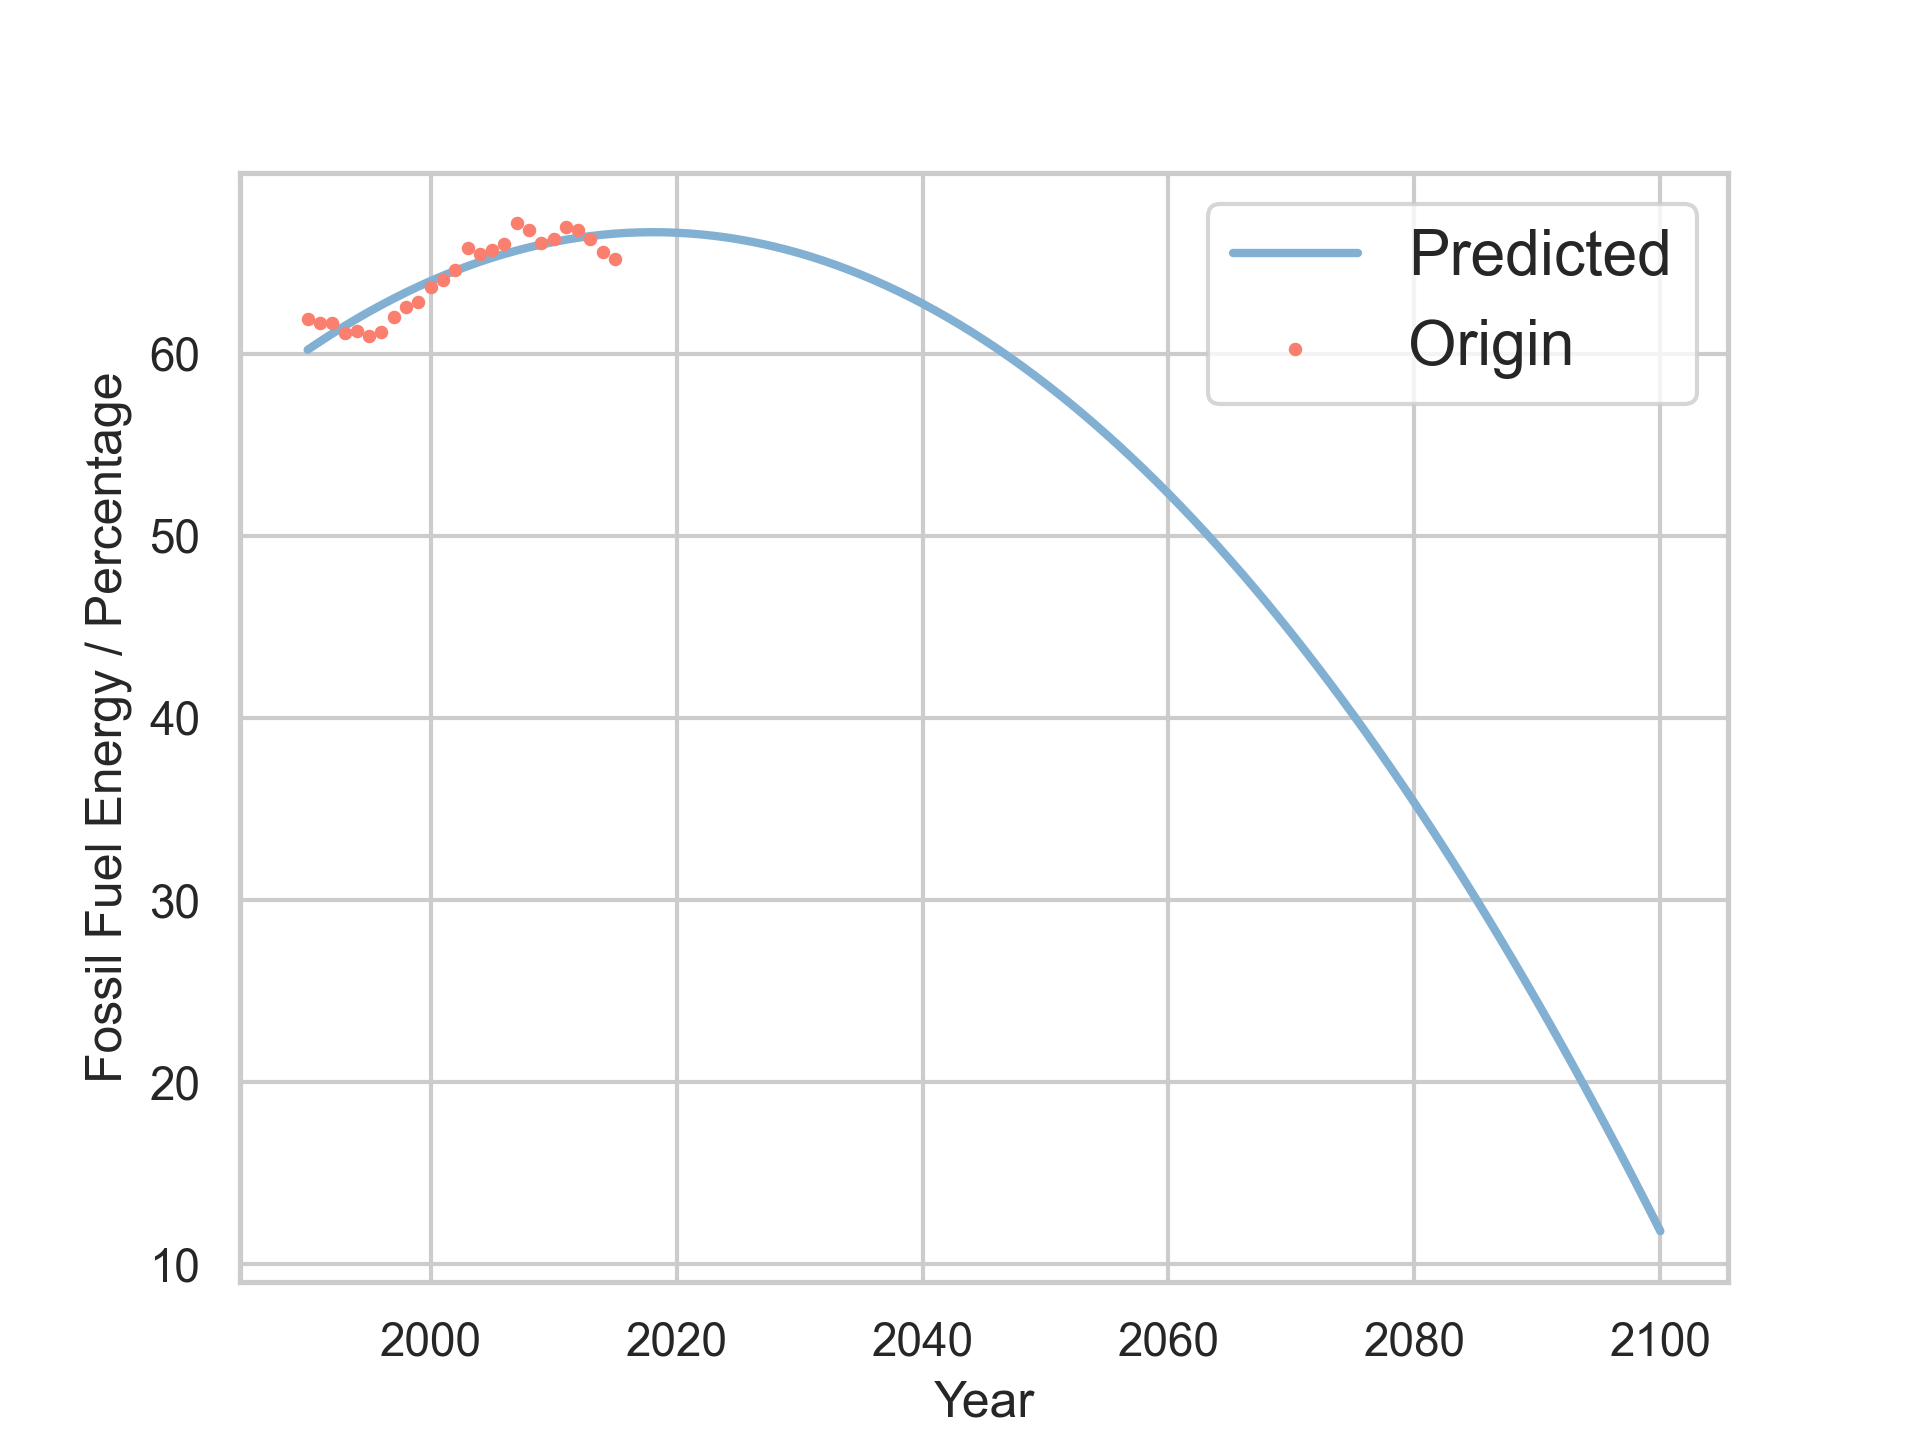
\includegraphics[width = \textwidth]{fig/projection/Energy_Production__Fossil_Fuel_().png}
            \caption{Fossil Fuel Energy Production (Percentage)}
        \end{subfigure}
    \caption{Predicted Energy Production Factors}
\end{figure}

Traditional industrial production makes up a major part of \ce{CO2} artificial release into the atmosphere. On the other hand, unlike production burning fossil fuel for energy, industrial activities using certain new forms of energy are considered carbon-free and thus greatly reducing \ce{CO2} levels. Although the construction of power generating infrastructures produces \ce{CO2}, new resources make considerable contributions in the long run. Wind, hydro and solar power and biomethane are typical renewable carbon-free energies. 

From a global point of view, power generation is currently at the dawn of carbon-free energies' prevalence. Renewable energies are generally passing experimental stage and entering the power market in certain areas. Thereby, we predicted the changes of energy quadratic functions, which fits the falling fossil fuel's percentage in energy production and the increasing trend of new energy production. 


\subsection{Model 1}
As mentioned above, we have picked ten representative factors for \ce{CO2} concentration $c$. Assuming $c$ be represented as the linear combination of the ten variables, \ce{CO2} concentration will be calculated by the formula below.

\begin{equation}
    c = \boldsymbol{k}_x \cdot \boldsymbol{x}^T    
\end{equation}

in which $\boldsymbol{k}_x$ and $\boldsymbol{x}$ are vectors respectively represent the weight of factors and the value of factors at some time. Thus, if given $\boldsymbol{k}_x$, we will be able to compute $c$ at any given moment. However, as many as ten variables will lead to unwanted disruption to the accuracy when deriving $\boldsymbol{k}_x$. So we have to first reduce the variables.

\subsubsection{Stage 1. Reducing Variables}

\textbf{Principle Components Analysis}, knows as \textbf{PCA}, is a model that reduces data points in a high-dimensional vector space to that in a lower dimensional one, while ensuring that the information they contain is expressed to the greatest extent. Here, we are going to reduce a $10$-dimensional vector (the ten factors mentioned before) to a $n$-dimensional one. 

Assume that the space where the original data points belong to is $V$, and the new space is $V'$. Generally, when applying PCA, we are in fact looking for a new set of 3 \textbf{basis} and extracting the original vectors' \textbf{projection} on this $n$-dimensional hyperplane. The PCA process is a linear transformation, which means it can be written in the following form:

\begin{equation}
    \label{PCA:main}
    W = M_{\text{pca}} \cdot X
\end{equation}

where $X$ is a $10$ by $m$ matrix ($m$ stands for the number of samples) and $W$ is a $3$ by $m$ matrix. To be specific, we select some vectors in $V$ to be the basis of $V'$. With the basis fixed, we then project the data points to $V'$, so that the new data points are now $n$-dimensional put to further use in the \ce{CO2} prediction.

When selecting the $k$-th vector, we first make show that the $k$-th vector is \textbf{linear independent} with the previous $k-1$ ones. Under that condition, We then pick the vector best representing information that are not carried by the first $k-1$ vectors.

To reflect how similar are the original variables, we introduce the concept of \textbf{covariance}. The covariance of two $n$-dimensional data points $\boldsymbol{a}$, $\boldsymbol{b}$ can be calculated with the following formula:

\begin{equation}
    Cov(\boldsymbol{a}, \boldsymbol{b}) = \frac{1}{n-1} \sum\limits_{i=1}^n 
    (\boldsymbol{a_i} - \bar{\boldsymbol{a}}) (\boldsymbol{b_i} - \bar{\boldsymbol{b}}) 
\end{equation}

where

\begin{equation}
    \bar{\boldsymbol{a}} = \frac 1 n \sum\limits_{i = 1}^n \boldsymbol{a_i}
\end{equation}

The covariance of more than two vectors is represented by a symmetric matrix $\Sigma$, which is given by the formula below:

\begin{equation}
    Cov(\boldsymbol{x_1} \cdots \boldsymbol{x_n}) = 
    \begin{bmatrix}
        Cov(\boldsymbol{x_1}, \boldsymbol{x_1}) & \cdots & Cov(\boldsymbol{x_1}, \boldsymbol{x_n}) \\
        \vdots & \ddots & \vdots \\
        Cov(\boldsymbol{x_n}, \boldsymbol{x_1}) & \cdots & Cov(\boldsymbol{x_n}, \boldsymbol{x_n})
    \end{bmatrix}
\end{equation}

The covariance of vectors, or data points, tells the how they are similar to each other. Thus, when choosing the basis of $V'$, we tend to choose less (for example, only one) to reflect the same message carried by a few original axes. To be specific, we first compute the covariance matrix of the uniformed data points. We then extract \textbf{eigenvector} and \textbf{eigenvalue} of the matrix, sort these eigenvalues from greatest to least, and pick corresponding \textbf{eigenvector} as the basis of $V'$. Later we compute the PCA matrix $M_{\text{pca}}$ and, with formula (\ref{PCA:main}), yield the result data $W$.

\subsubsection{Stage 2. Fit 3 Variables into 1}
\label{m1:sec:mr}

Having reduced 10 variables to 3, we can now use \textbf{Multivariate Regression} to derive the relationship between \ce{CO2} concentration $c$ and $\boldsymbol{w}$. Multivariate regression is a widely adapted algorithm that allows people to establish the relationship between a dependent variable and a set of independent variables. The algorithm can help us extract a linear function of the independent variables that fit our given data relatively well. 

To measure the how well a function is in accord with the data, we introduce the \textbf{loss function}. Let the loss function be calculated by the following formula:

\begin{equation}
    L(\boldsymbol{c}, \hat{\boldsymbol{c}}) = \frac 1 {2m} \sum\limits_{i=1}^m
    (c_i - \hat c_i)^2
\end{equation}

The less $L$ be, the better does our function fit into given data. Adapting optimization algorithms like \textbf{Gradient Descent}, we can minimize $L$ and derive the analytic expression of our best function. The function reflects the relationship between $c$ and $\boldsymbol{w}$, and can be used to predicit the future trend of $c$. The function can be expressed in the following form:

\begin{equation}
    \label{MR:main}
    c = f_{\text{mr}} (\boldsymbol{w}) = \boldsymbol{k}_{mr} \cdot \boldsymbol{w}^T
\end{equation}

\subsubsection{Stage 3. Compute the Result}

Substituting formula (\ref{MR:main}) into (\ref{PCA:main}), we obtain the relationship between $c$ and $\boldsymbol{x}$. Obviously, $c$ is a linear combination of $\boldsymbol{x}$. Thus, 

\begin{equation}
    \label{m1:main}
    c = \boldsymbol{k}_{m1} \cdot \boldsymbol{x}
\end{equation}

where

\begin{equation}
    \boldsymbol{k}_{m1} = \boldsymbol{k}_{mr} \cdot M_{\text{pca}}
\end{equation}

We then combine the projections of $\boldsymbol{x}$, which have been demonstrated in section \ref{factors}, with equation (\ref{m1:main}), so that the future projection of $c$ can be computed. Prediciton of this model is showed in Figure. \ref{m1:fig}.

\begin{figure}[hbt]
    \centering
    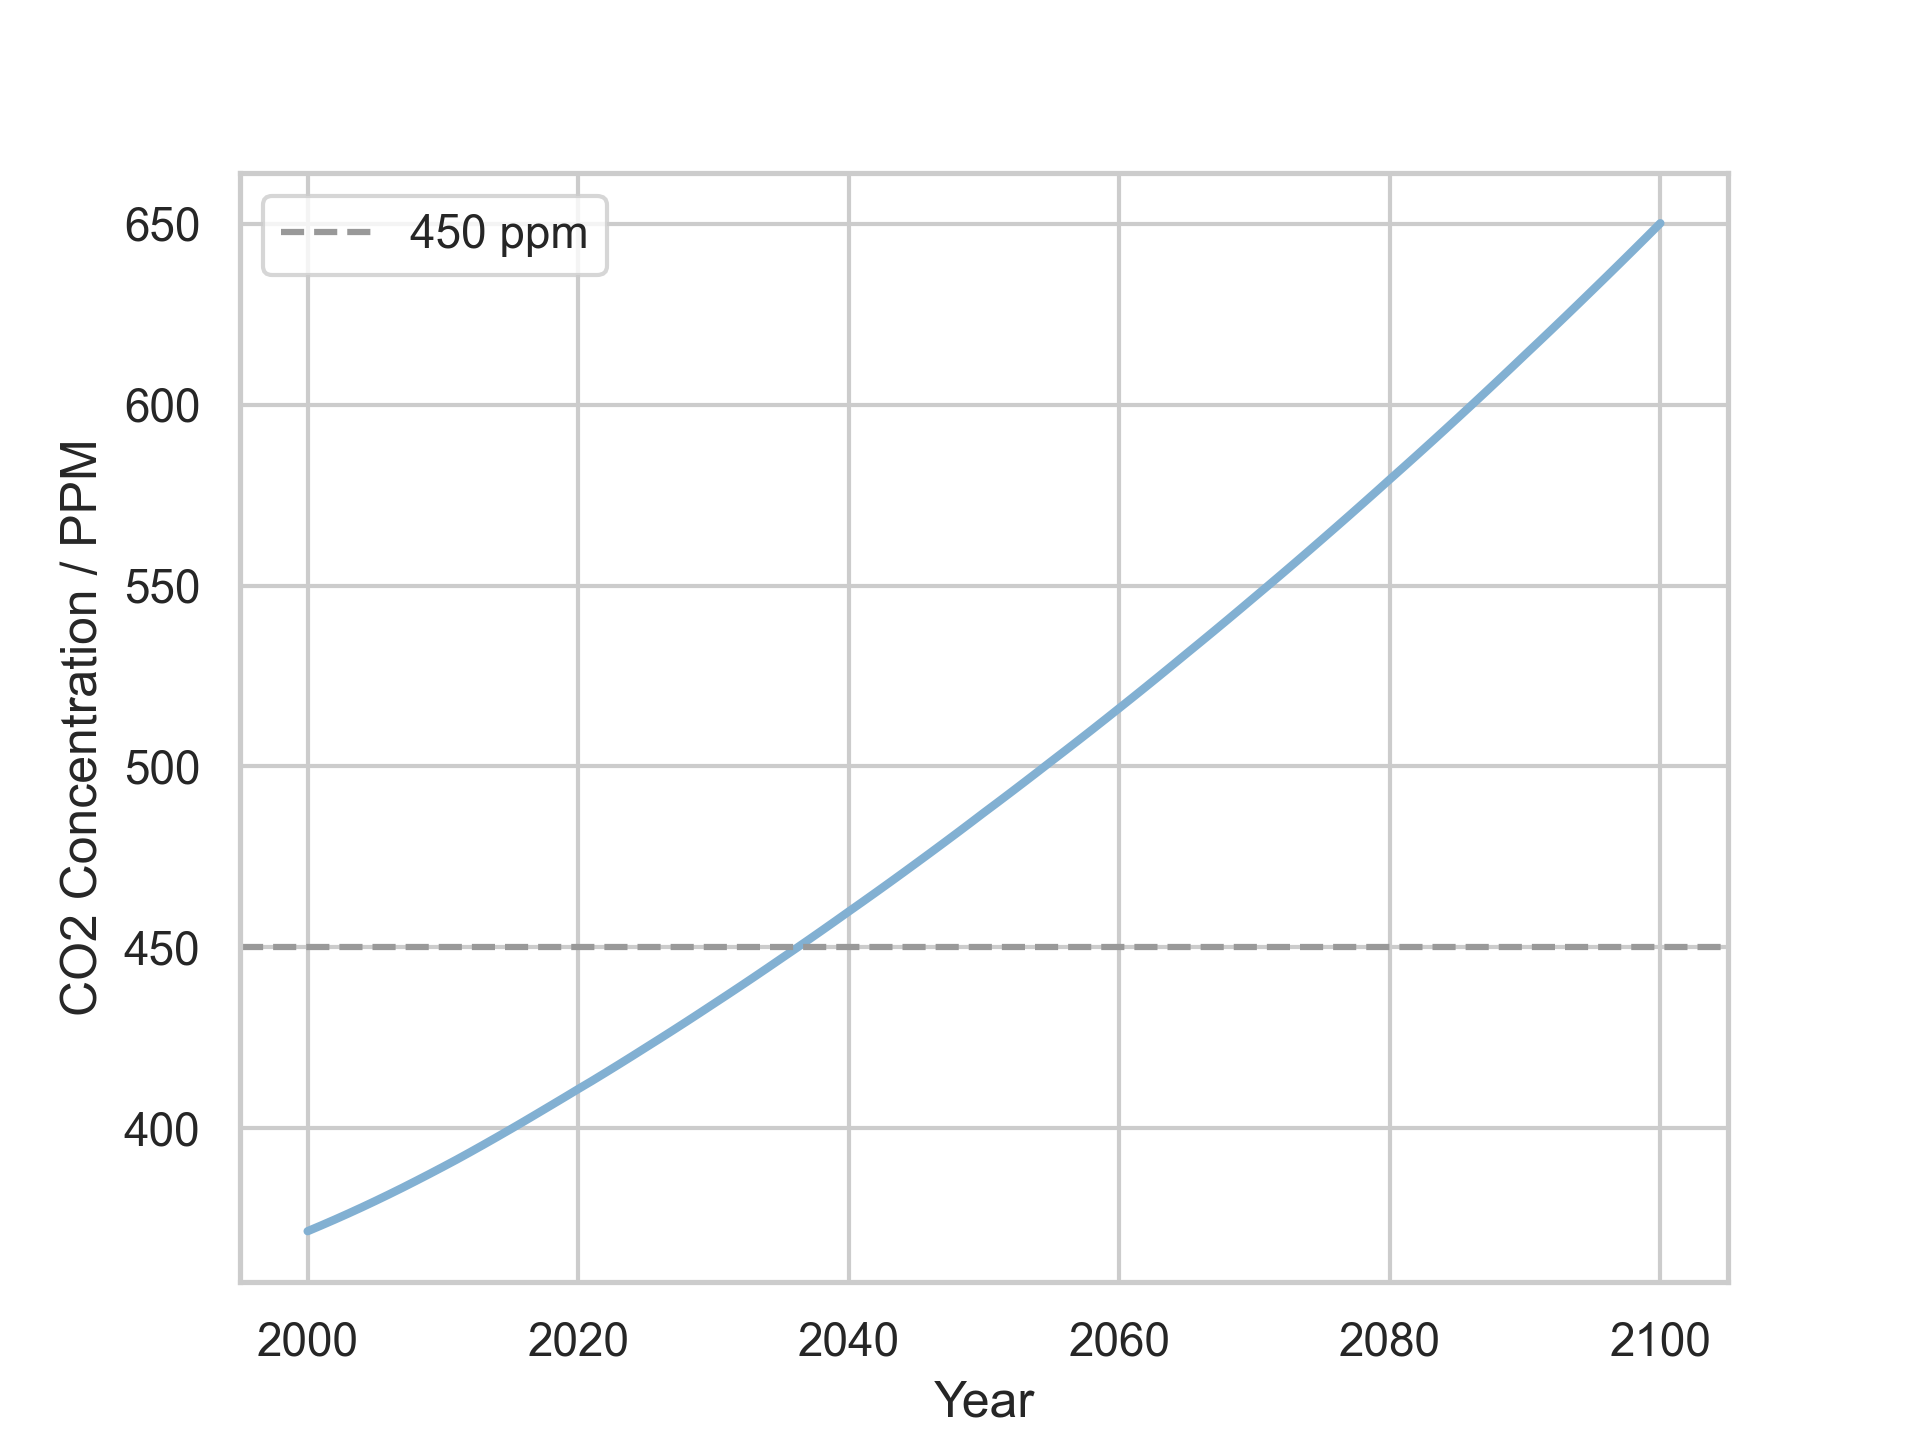
\includegraphics[width = 0.7\textwidth]{fig/PCA.png}
    \caption{\ce{CO2} Concentraion Projection by Model 1}
    \label{m1:fig}
\end{figure}

\subsection{Model 2}

\subsubsection{Stage 1. Picking 3 Variables with Stepwise Regression}

Since putting too many variables into multivariate may yield a function far from comprehensive, or \textbf{overfitted}, we should first pick some variables with the deepest and most irreplaceable impacts on the dependent variable $c$ prior to the simulation. Here, the \textbf{Stepwise Regression} algorithm allows us to pick the most important variables. 

To quantify the severity of \textbf{multicollinearity} (in other words, dependence) in a regression model, we introduce the \textbf{Variance Inflation Factor} (\textbf{VIF}) index, which is given by the formula (\ref{VIF}). 

\begin{equation}
    \text{VIF} = \frac{1}{1 - R^2}
    \label{VIF}
\end{equation}

in which $R^2$ is the \textbf{Coefficient of Determination} of the regression model, reflecting the level the model fits into the data. $R^2$ of a dataset $\boldsymbol{y}$ is determined by the formula (\ref{R2}). Assume that $\bar y$ is the mean of $\boldsymbol{y}$ and $\hat{y}$ is the predicted value of $\boldsymbol{y}$.

\begin{equation}
    R^2 = 1 - \frac{SS_{\text{res}}}{SS_{\text{tot}}}
    \label{R2}
\end{equation}

where

\begin{equation}
    SS_{\text{res}} = \sum\limits_{k} (\hat y_k - y_k) ^ 2
\end{equation}
\begin{equation}
    SS_{\text{tot}} = \sum\limits_{k} (\bar y_k - y_k) ^ 2
\end{equation}

When selecting variables from the original ten variables, we first adapt multivariate regression (which has been illustrated in section \ref{m1:sec:mr}) to generate a regression model and compute its $\text{VIF}$. If $\text{VIF}$ is too large (for example $\text{VIF} \ge 10$), we discard this variable. At last, three variables are selected, which are:

\begin{itemize}
    \item \textbf{Global population} $x_1$
    \item \textbf{Energy production: fossil fuel} (Percentage) $x_6$
    \item \textbf{Energy production: new energy} $x_7$
\end{itemize}

\subsubsection{Stage 2. Predicting $c$ with STIRPAT Equation}
The \textbf{IPAT Equation} is a model developed in 1970, during a debate on how technological development impact the environment. The equation quantify human's impacts($I$) on the environment by multiplying indexes of population($P$), affluence($A$) and technology($T$). Thus, 

\begin{equation}
    I = P \times A \times T
\end{equation}

In 2003, A Rosa and Dietz perfected the model by transforming the IPAT equation to an exponential equation, developing the \textbf{ST}ochastic \textbf{I}mpacts by \textbf{R}egression on \textbf{P}opulation, \textbf{A}ffluence, and \textbf{T}echnology (\textbf{STIRPAT}) analysis\cite{STI}. The \textbf{STIRPAT Equation} is shown in formula (\ref{m3:STI}).

\begin{equation}
    \label{m3:STI}
    I = a P^{\alpha} A^{\beta} T^{\chi} e
\end{equation}

In the light of this, we adapt a similar equation to model $x_1$, $x_6$ and $x_7$'s impact on $c$, which is displayed below.

\begin{equation}
    \label{m2:st0}
    c = a \times {x_1}^\alpha \times {x_6}^\beta \times {x_7}^\chi \times e
\end{equation}

Transform all variables to logarithmic form, we have

\begin{equation}
    \label{m2:st}
    \ln c = \ln a + \alpha \ln{x_1} + \beta \ln{x_6} + \chi \ln{x_7} + \ln e
\end{equation}

Equation (\ref{m2:st}) illustrates that a \textbf{linear relationship} between $\ln c$ and $\ln x$ exists. Hence, we can use \textbf{Multivariate Regression} to estimate the relationship between $ln c$ and $\ln x$, and then yield the function to predict $c$'s changes in the future. After performing multivariate regression (thus, deriving $\ln a, \alpha, \beta, \chi$ and $\ln e$), we can calculate $c$ with formula (\ref{m2:st0}). The result is displayed in Figure. \ref{m2:fig}.

\begin{figure}[hbt]
    \centering
    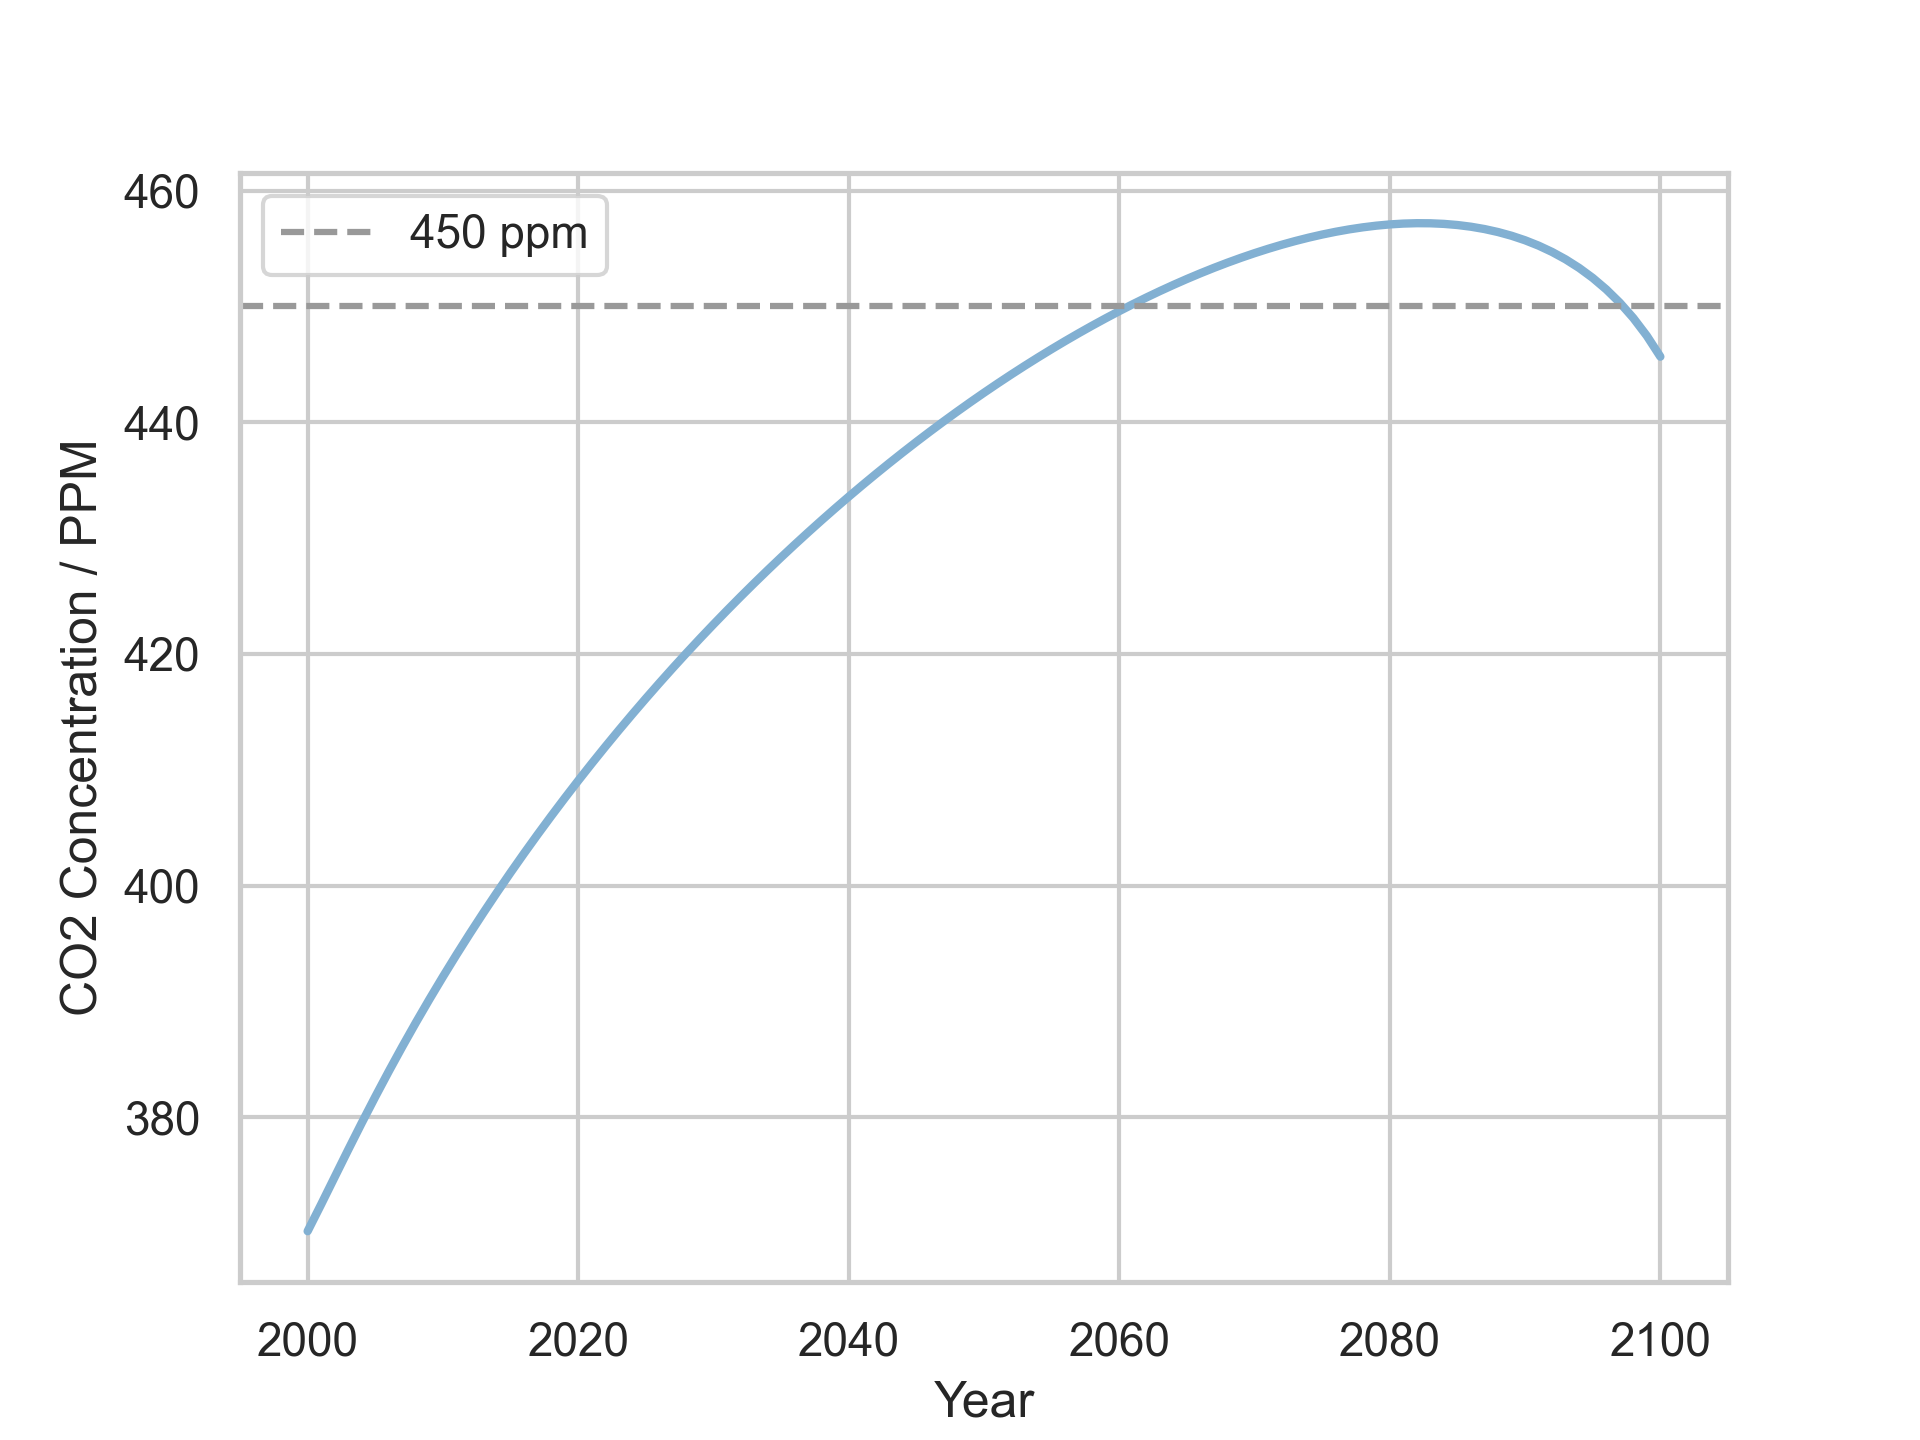
\includegraphics[width = 0.7\textwidth]{fig/STI.png}
    \caption{\ce{CO2} Concentraion Projection by Model 2}
    \label{m2:fig}
\end{figure}

\subsection{Model 3}
\label{m3}

\subsubsection{Stage 1. Considering a Differential Equation Model}

As is clear from the past data, \ce{CO2} concentration in the atmosphere is significantly influenced by human activities. while artificial carbon emission is also affected by \ce{CO2} concentration. Thus, a retroaction effect exists between human activities and \ce{CO2} concentration.

Since $c$ and $t$ respectively represent \ce{CO2} concentration and time, $\frac{\mathrm{d}c}{\mathrm{d}t}$ stands for the amount of \ce{CO2} emitted at a certain moment. In the light this, we can adapt \textbf{Ordinary Differential Equation} (aka \textbf{ODE}) to model the retroaction effect mentioned above. Generally, the equation can be written in the form below:

% \begin{equation}
\begin{align}
    \label{ODE:big}
    \frac{\mathrm{d}c}{\mathrm{d}t} & = f_{p0}(c, t)\\
    & = f_c(c) + f_t(t)
\end{align}
% \end{equation}

where the function $f_c$ reflects the \ce{CO2} concentration on human activity, and function $f_t$ generally reflects the opposite effect. After determining function $f_c$ and $f_t$ (we name them \textbf{Feedback Functions}), we will then solve the differential equation and thereby derive the relationship between $c$ and $t$. 

\subsubsection{Stage 2. Establishing the Feedback Functions}

\paragraph{Human Activities Feedback}
In order to model how human activities affect carbon emission, we selected 3 key factors, which are:

\begin{itemize}
    \item \textbf{Global population} $x_1$
    \item \textbf{Urban population} $x_2$
    \item Percentage of \textbf{fossil fuel energy production} in overall energy production $x_6$
\end{itemize}

As we can see in the data from the past, developed and developing counrties varies in carbon emission per capita. This implies that generally there is a large carbon-emission gap between urban areas and suburban. This gap remind us to consider population of different areas respectively. 
Also, energy production is a major source of carbon emission today -- In 2021, $62\%$ of global energy production is contributed by fossil fuel, which occupies $20\%$ of industrial carbon emission. 

We then use the 3 selected variables to determine $f_t$, the human activity feedback function. Subtracting $x_2$ from $x_1$, we can compute the number of non-urban population. We then multuply the vector $[x_1, x_2 - x_1, x_6]$ by some coefficient ${\boldsymbol{k}_\text{fh}}$ (which is also a vector) and derive the value of $f_c(t)$ at some certain moment $t$.

\begin{equation}
\label{ODE:ft}
f_t(t) = [x_1, x_2 - x_1, x_6] \cdot {\boldsymbol{k}_\text{fh}}
\end{equation}

However, only for $t \in \mathbb{Z}$ is this formula correct, for that $x_1$, $x_2$ and $x_6$ are discrete sequences. In order to derive a continuous function (for the propose of solving differential equation), we fit the sequences of $f_t(t), t \in \mathbb{Z}, t \in [1960, 2021]$ with a cubic polynomial. The function holds for $t \in \mathbb{R}, t \in [1960, 2021]$. Thus, 

\begin{equation}
    \label{ODE:ft2}
    f_t(t) \approx p_a t^2 + p_b t + p_c
\end{equation}

\paragraph{\ce{CO2} Concentraion Feedback}
To model the changes that increasing \ce{CO2} concentration will bring to human activities, we assume that once \ce{CO2} concentration in the atmosphere reaches a certain level, humans will establish hardened policies to keep \ce{CO2} emission within limits. In our projection, we set this limit $L$ as $450$ PPM\cite{ref450}. The \ce{CO2} Feedback Function is organized as follow, 

\begin{equation}
    \label{ODE:fc}
    f_c(c) = 
    \begin{cases}
        k_{fc} \cdot c^2 & c \le L\\
        p_{d} \cdot \exp((p_e \cdot c + p_f)) + p_g & c > L
    \end{cases}
\end{equation}

Since the $\exp$ function grows much faster than the quadratic function, the formula above characterizes how human activities are affected by \ce{CO2} emission with relatively high accuracy.

\subsubsection{Stage 3. Solve the Differential Equation}

With the method to compute Feedback Functions clearly established, we are now fully enabled to solve the differential equation. Substituting formula (\ref{ODE:ft2}), (\ref{ODE:fc}) into (\ref{ODE:big}), we have

\begin{equation}
    \label{ODE:ODE}
    \frac{\mathrm{d}c}{\mathrm{d}t} =
    \begin{cases}
        p_a t^2 + p_b t + p_c \ + \ k_{fc} \cdot c^2 & c \le L\\
        p_a t^2 + p_b t + p_c \ + \ p_{d} \cdot \exp((p_e \cdot c + p_f)) + p_g & c > L
    \end{cases}
\end{equation}

Upon solving this equation, we can derive the relationship between $c$ and $t$. The result is showed in the Figure. \ref{m3:fig}.

\begin{figure}[hbt]
\centering
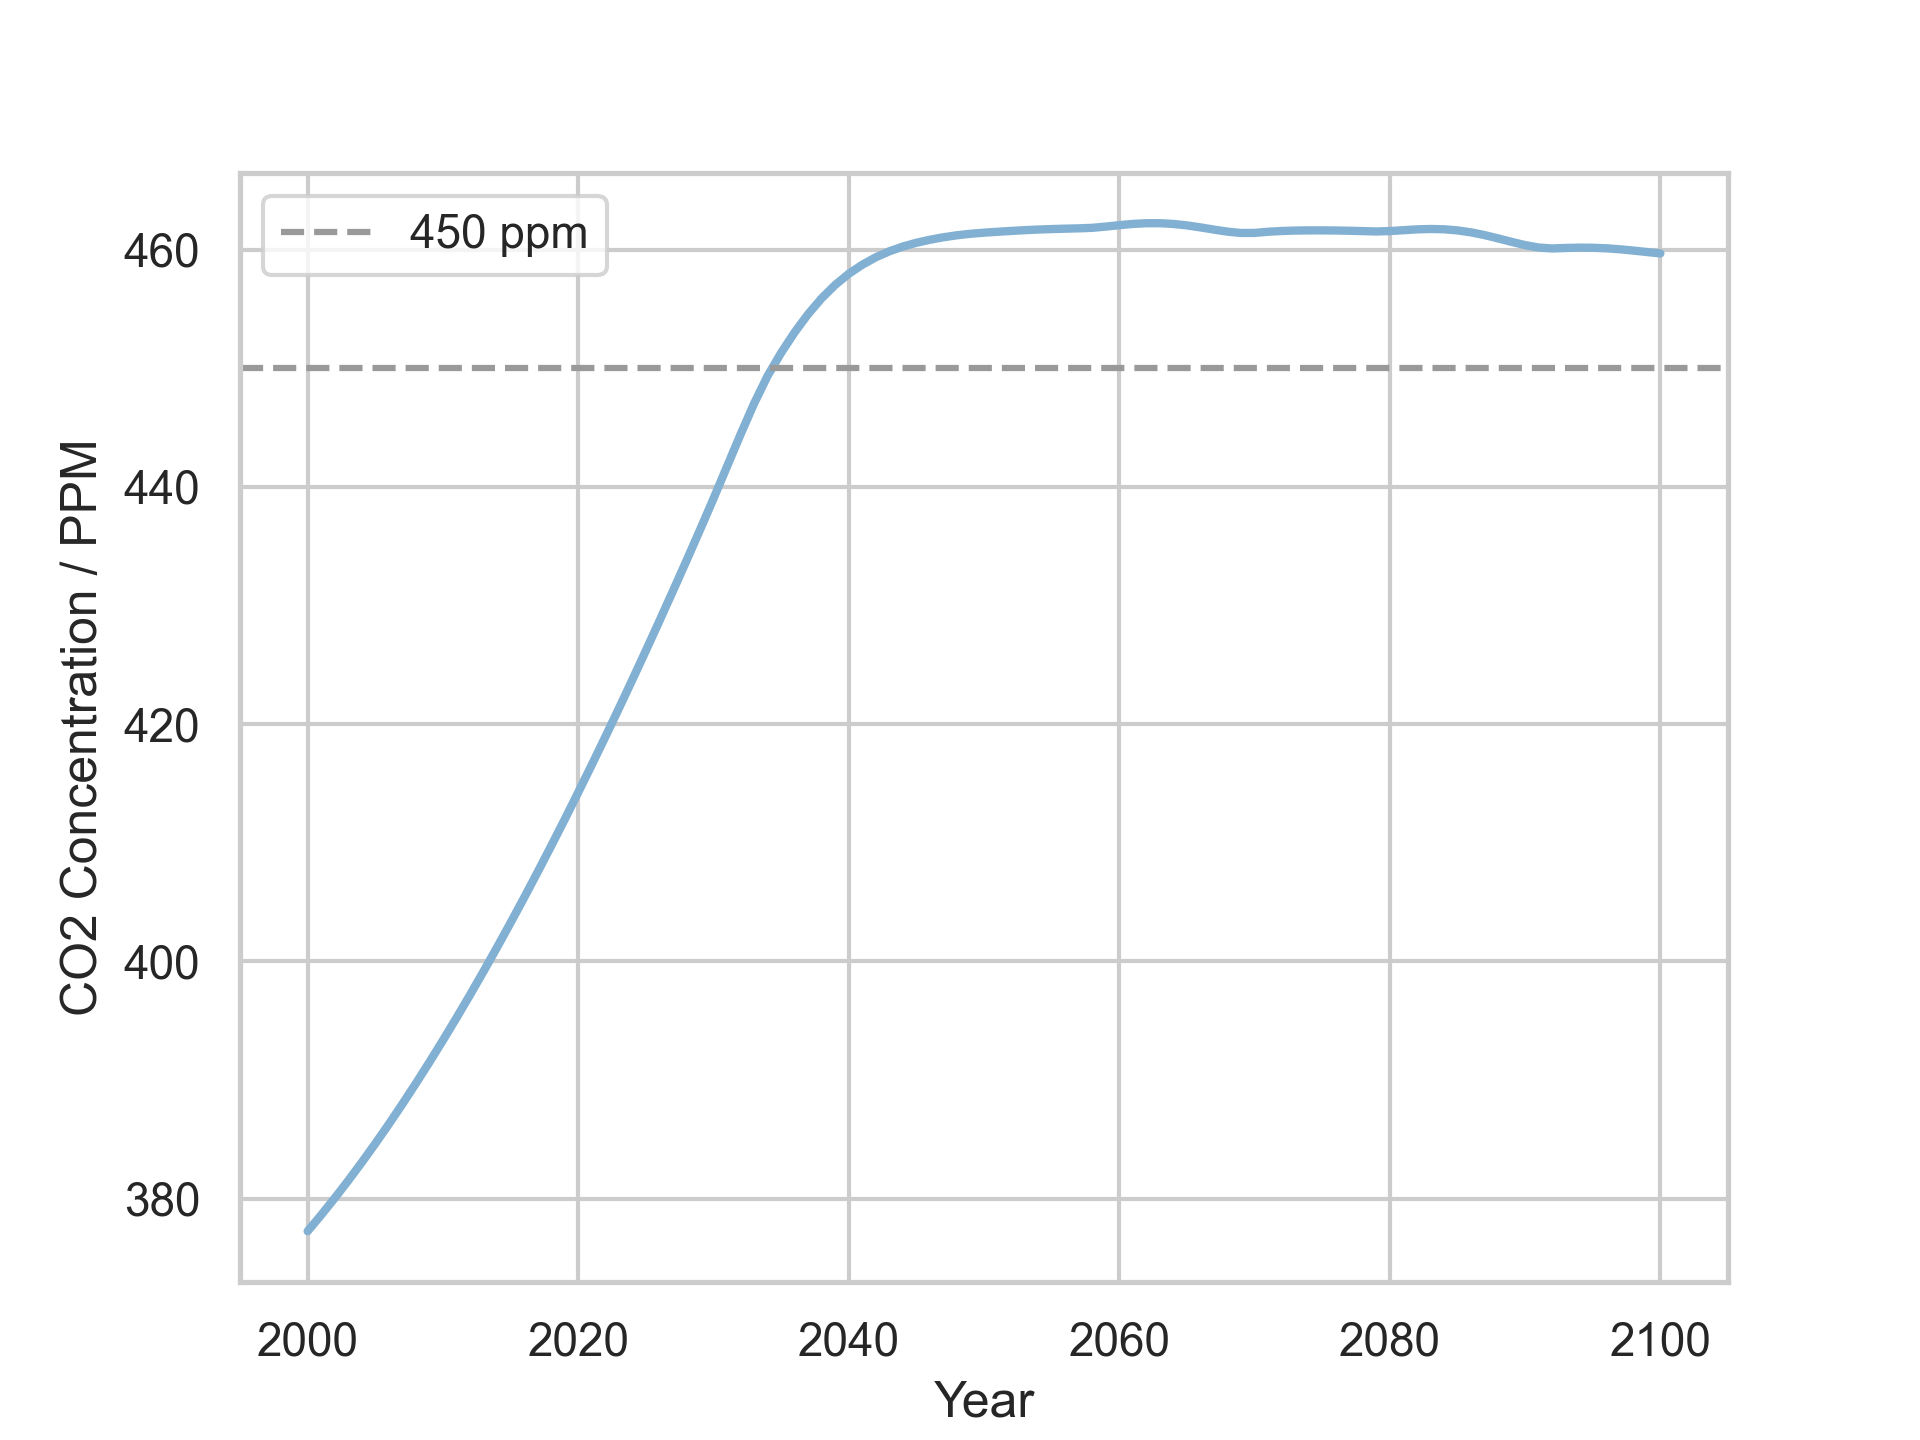
\includegraphics[width = 0.7\textwidth]{fig/ODE.png}
\caption{\ce{CO2} Concentraion Projection by Model 3}
\label{m3:fig}
\end{figure}

The dashed line marks $c=450$ PPM. From the Figure.\ref{m3:fig} we can see that before \ce{CO2} concentration reaches $450$ PPM, it grows at a constant rate year by year. However, when \ce{CO2} concentration goes above, its slope begins to decrease due to humans' control of \ce{CO2} emission. After the year 2045, \ce{CO2} level in the atmosphere stays around $460$ PPM relatively constantly, for that in this level, \ce{CO2} generally exert little negative influence on the environment.


\section{Methodology: Problem 2}
\label{method:2}

\subsection{Model 4: Prediction Temperature Trends}

As shown in Figure.\ref{smooth}, annual mean temperature shifts dramatically from year to year, yet an overall rising trend can be observed. In order to simplify and describe the changes, we applied \textbf{Lowess Smoothing}. This algorithm allows us to smoothen a curve and extract its inclination. Figure.\ref{smooth} show the effect of lowess smoothing algorithm. 

\begin{figure}[hbt]
    \centering
    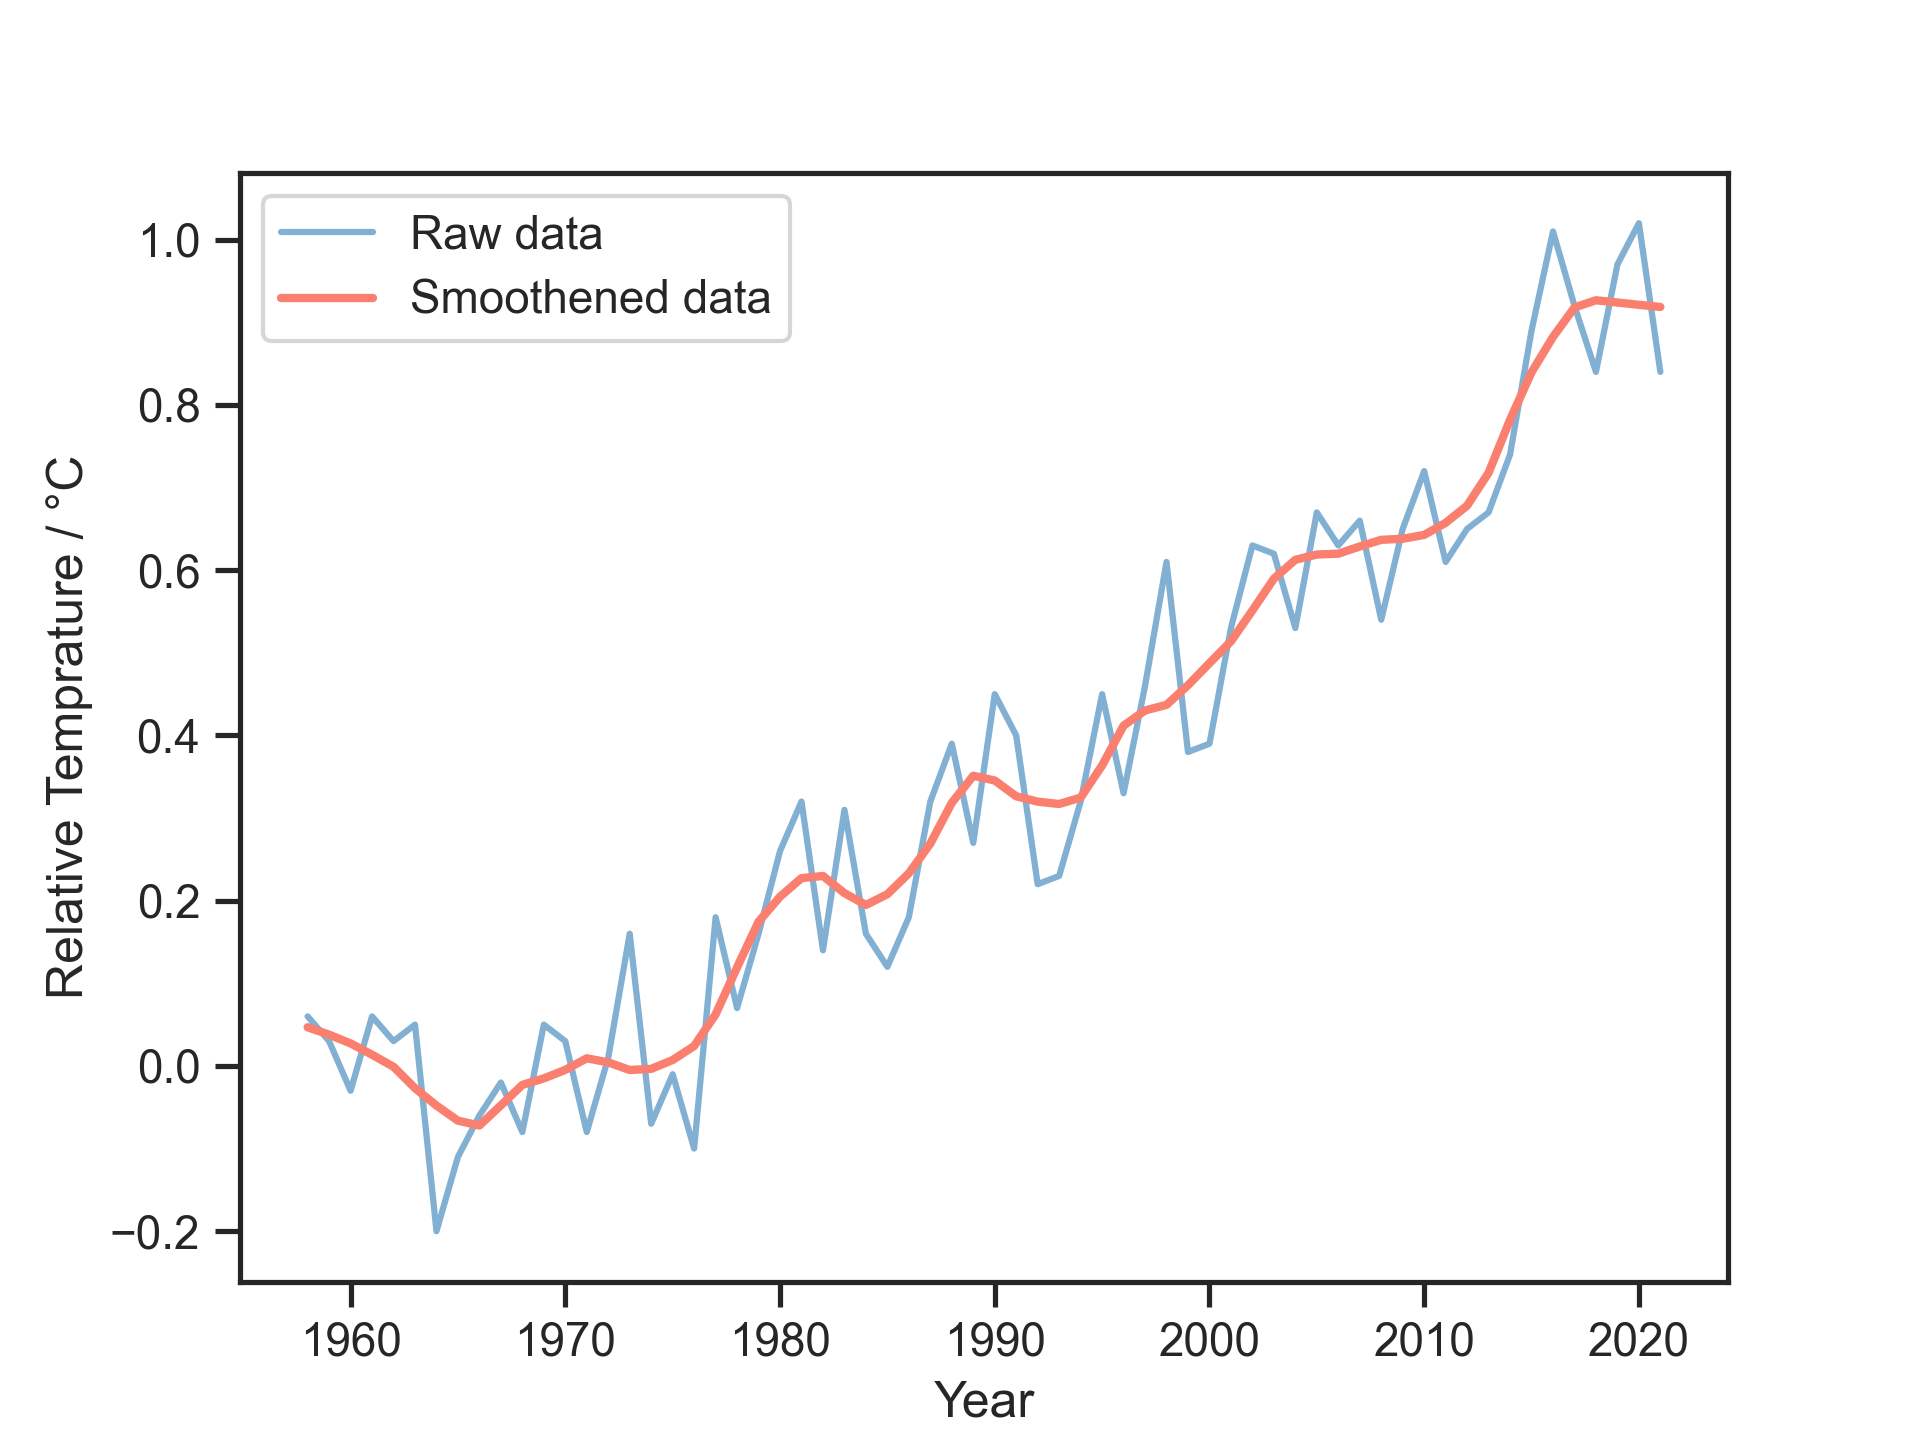
\includegraphics[width = 0.7\textwidth]{fig/Lowess.png}
    \caption{Comparison between raw data and smoothed data}
    \label{smooth}
\end{figure}

Let $\boldsymbol{x}$ and $\boldsymbol{y}$ be the raw data, and $\boldsymbol{y}_{\text{ls}}$ be the Lowess smoothened data. When we apply Lowess Smoothing, the following steps are taken.

\begin{itemize}
    \item \textbf{Step 1.} Establish a weight function $w(\boldsymbol{x})$.
    \item \textbf{Step 2.} Implement the following steps for every $x_i \in \boldsymbol{x}$: 
    \begin{itemize}
        \item \textbf{Step 2.1.} Take a neibouring interval of $x_i$. Name the interval $A$.
        \item \textbf{Step 2.2.} Fetch every $x_k \in A$ and derive $w(x_k)$. Stack $x_k$ together to get $\boldsymbol{x}_{\text{part}}$. Name the corresponding parts of $\boldsymbol{y}$ as $\boldsymbol{y}_{\text{part}}$.
        \item \textbf{Step 2.3.} Implement Linear Regression for $\boldsymbol{x}_{\text{part}}$ and $\boldsymbol{y}_{\text{part}}$. 
        \item \textbf{Step 2.4.} Take the \textbf{mid point} of the regression line $\hat y$ as $y_{\text{ls}i}$. 
    \end{itemize}
    \item \textbf{Step 3.} Stack $y_{\text{ls}i}$ for every $i$ together to yield $\boldsymbol{y}_\text{ls}$.
\end{itemize}

After performing Lowess Smoothing, we designed a special function to fit the smoothened curve. We notice that the curve is generally growing at an increasing rate, which is in accord with the pattern of a quadratic function. Also, we observe that the vibration in land-ocean temperature follows a certain periodical pattern. According to NASA-JPL, solar activity exerts influences on earth temperature -- solar activity intensitiy and land-ocean temperature on earth share peaks and troughs. As intensity of solar activity follows the 11-year period, we adapt three sine functions respectively, with their periods set to $10$, $11$ and $12$. Hence $\omega_1=\frac{2\pi}{10}$, $\omega_2 = \frac{2\pi}{11}$ and $\omega_3 = \frac{2\pi}{12}$. Finally, our function to fit the temperature curve is:

\begin{equation}
    \label{2a:main}
    h(t) = p_1 t^2 + p_2 t + p_3\sin(\omega_1 t + p_5) + p_6\sin(\omega_2 t + p_7) + p_8\sin(\omega_3 t + p_9) + p_{10}
\end{equation}

Applying Ordinary Least Squares method, we yield the coefficient $p_1 \sim p_12$. Prediction of $c$ made by this function is shown in Figure.\ref{2a:fig}.

\begin{figure}[hbt]
    \centering
    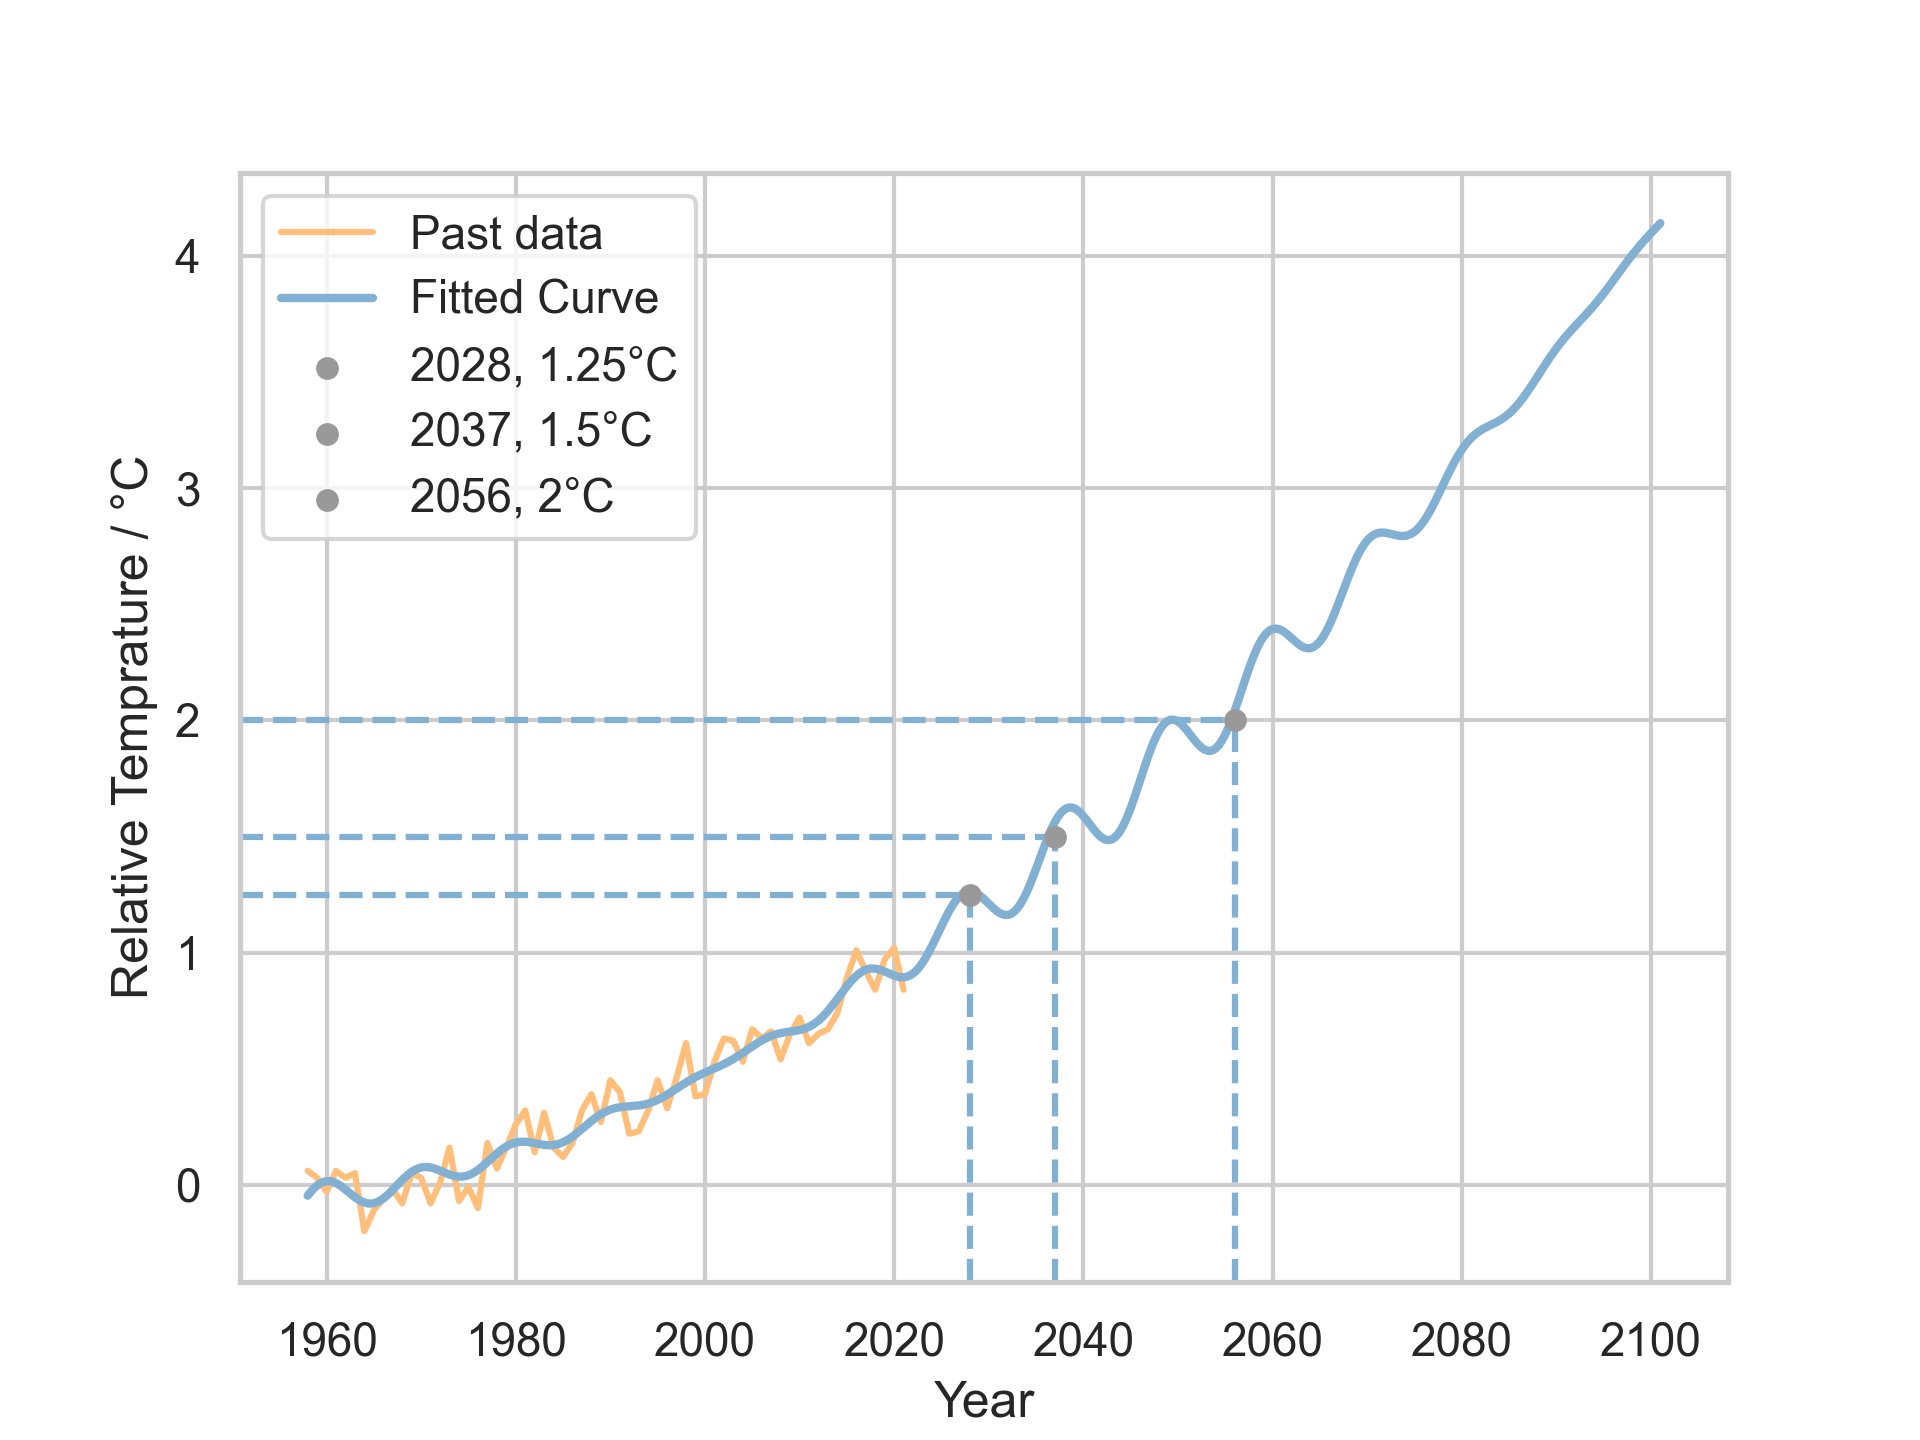
\includegraphics[width = 0.7\textwidth]{fig/2a_prediction.png}
    \caption{Land-ocean Temperature Projection by Model 4}
    \label{2a:fig}
\end{figure}

As displayed in Figure.\ref{2a:fig}, the land-ocean temperature keeps rising and vibrating. According to our prediction, earth temperature(relative) will raise $1^{\circ}$C by 2028, $1.25^\circ$ by 2037 and $2^\circ$C by 2056. 

\subsection{Model 5: Measuring Relationship between Temperature and \ce{CO2}}

\subsubsection{Qualitative Analysis}

In order to study whether \ce{CO2} is a major factor causing global warming, we collect 6 variables that may have impacts on land-ocean temperature, including

\begin{itemize}
    \item number of sunspots $z_1$
    \item all sky surface shortwave downward irradiance (SWDR) $z_2$ (in $W / m^2$)
    \item outgoing longwave radiation irradiance (OLR) $z_3$ (in $W / m^2$)
    \item \ce{CO2} concentration in atmosphere $z_4$ (in PPM)
    \item \ce{CH4} concentration in atmosphere $z_5$ (in PPM)
    \item \ce{N2O} concentration in atmosphere $z_6$ (in PPM)
\end{itemize}

Among these variables, $z_1$, $z_2$ and $z_3$ are connected to solar activities and radiation, while $z_4$, $z_5$ and $z_6$ discribe greenhouse gases. To find out which of the factors bear the most severest impacts on temperature, we adapt the \textbf{Grey Relational Analysis} method. The algorithm allows us to calculate the \textbf{Grey Relational Grade} (\textbf{GRG}), which quantifies the correlation between our measurement facters($Z$) and the target sequences $\boldsymbol{c}$. 

To calculate GRG, we have to first yield the \textbf{Grey Relational Coefficients}  (\textbf{GRC}). We calculate GRC between the $i$-th factor($z_i$) and the target$z_0$ on $k$-th data point, which is referred to as $\zeta_i(k)$, with formula (\ref{zeta}).

\begin{equation}
    \label{zeta}
    \zeta_i(k) = \frac{
        \min_i \min_k | z_0(k) - z_i(k) | + r \cdot
        \max_i \max_k | z_0(k) - z_i(k) |
    }{
        | z_0(k) - z_i(k) | + r \cdot
        \max_i \max_k | z_0(k) - z_i(k) |
    }
\end{equation}

Later, we can calculate GRG of some factor $z_i$:

\begin{equation}
    \text{GRG}_i = \frac 1 m \sum\limits_{k=1}^m \zeta_i(k)
\end{equation}

Based on data ranging from 1959 to 2021, we compute GRG for $z_1 \sim z_6$. The computation result is displayed in Figure.\ref{GRG}.

\begin{figure}[hbt]
    \centering
    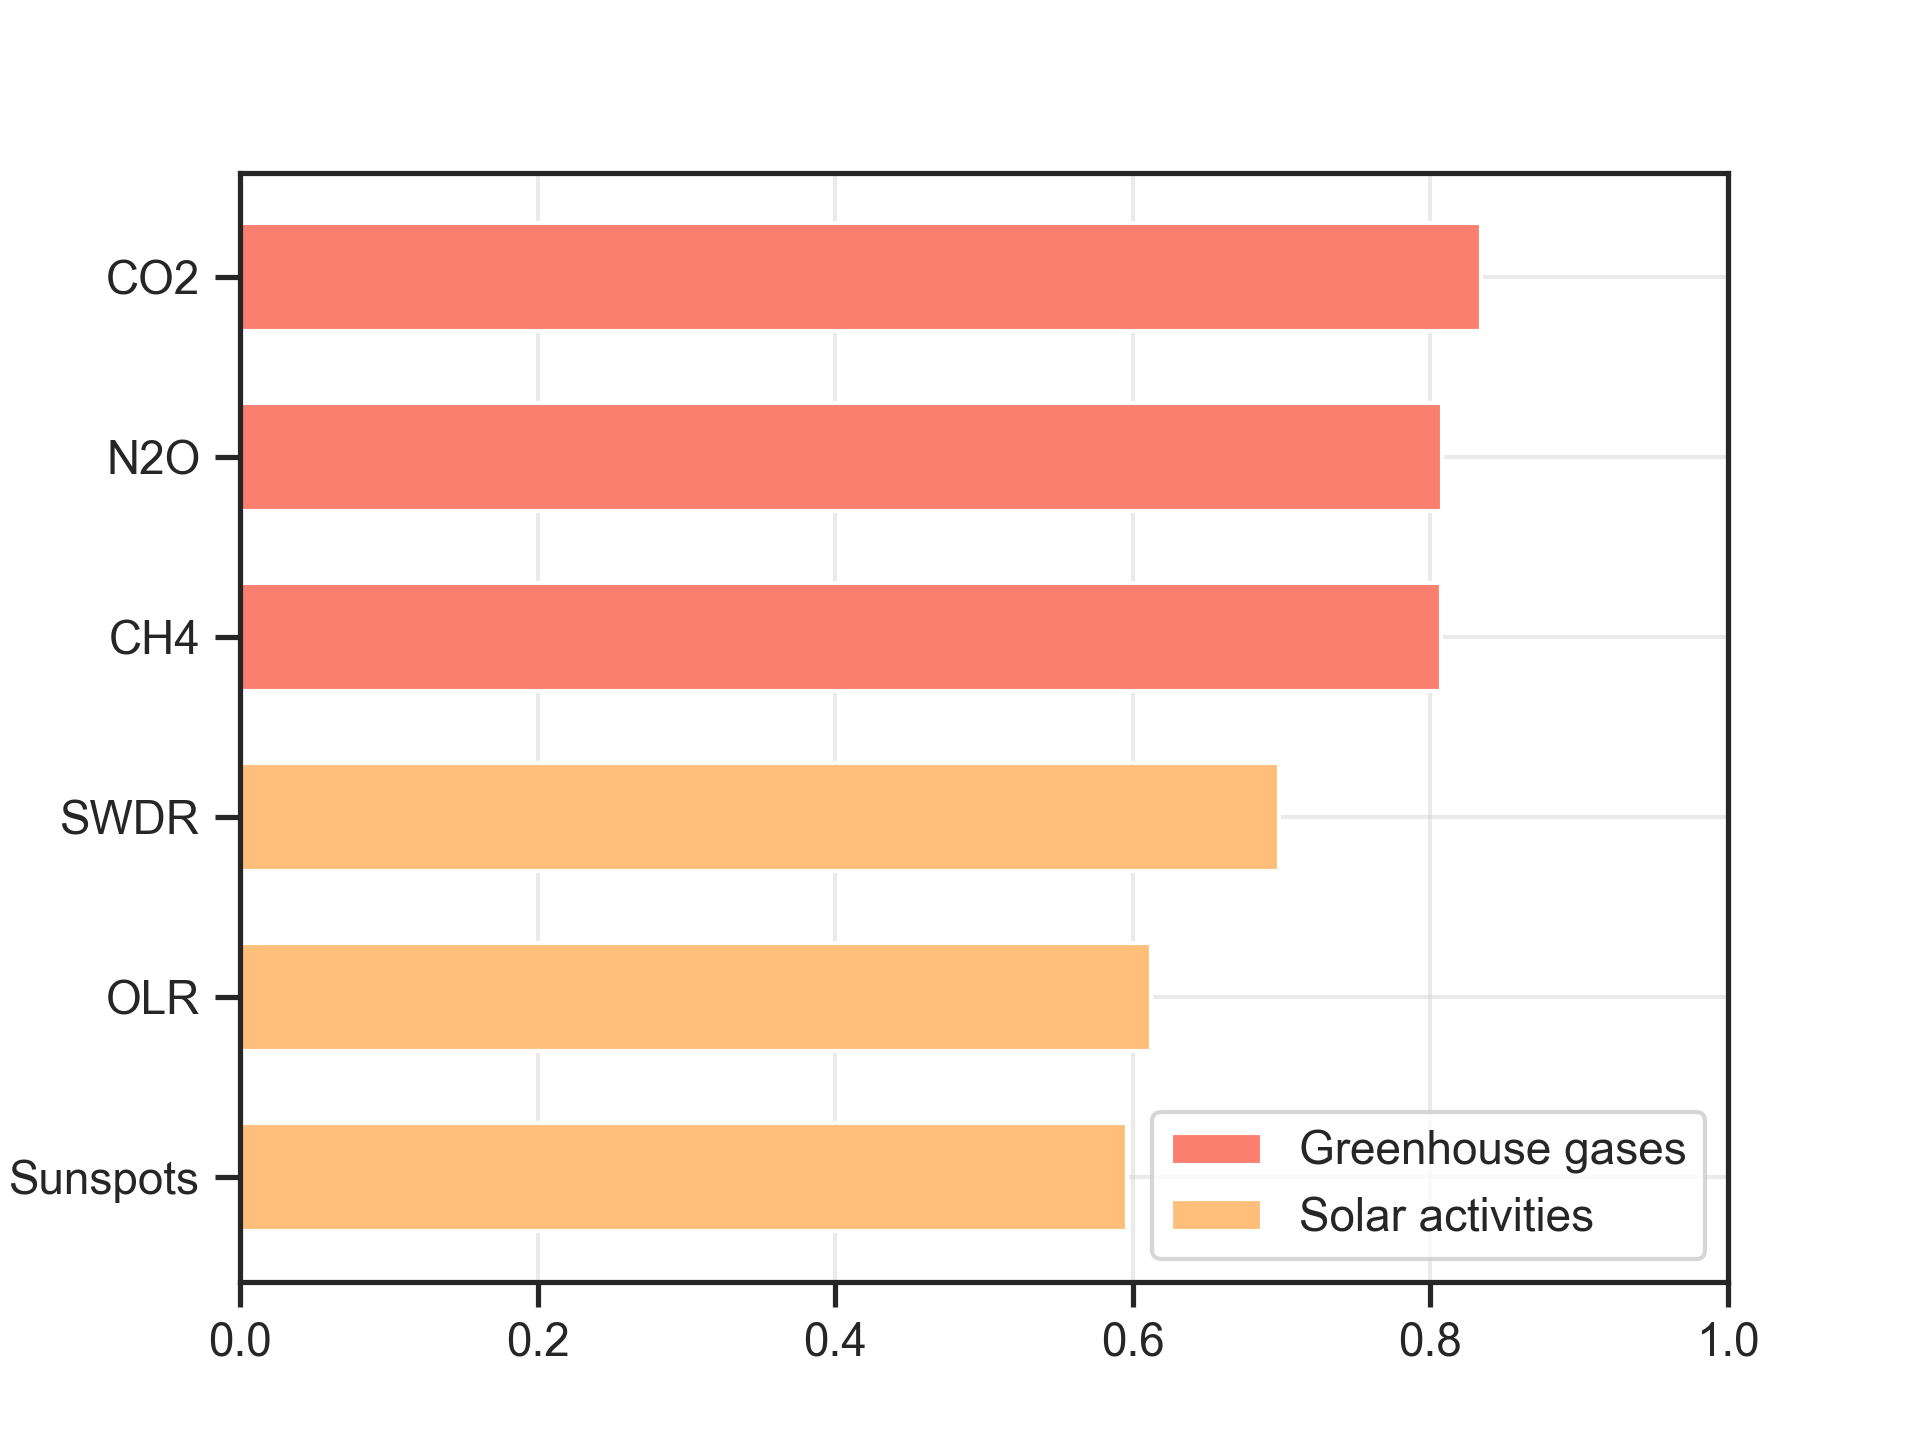
\includegraphics[width = 0.7\textwidth]{fig/original_2b.png}
    \caption{GRG of 6 factors $z_1 \sim z_6$}
    \label{GRG}
\end{figure}

As shown in Figure.\ref{GRG}, the three greenhouse gases are all closely related to land-ocean temperature changes, while the impacts from solar activities are less significant. Among all the greenhouse gases, GRG of \ce{CO2} is the greatest, which convinced us that \ce{CO2} is a major factor accelerating global warming. 

\subsubsection{Quantitative Analysis}

To measure the impacts of \ce{CO2} on land-ocean temperature and how the impacts vary in a wider range of time, we introduce the \textbf{Spearman's coefficient} $\rho$, which reflects how closer the two variable are related with each other. The Spearman's coefficient gives a number between $-1$ and $1$. The more closely the two variables are related, the smaller $|1 - \rho|$ will be. This coefficient is determined by the following formula. 

\begin{equation}
    \rho(\boldsymbol{a}, \boldsymbol{b}) = \frac{\sum\limits_i (a_i - \bar a)(b_i - \bar b) }{\sqrt{
        \sum\limits_i (a_i - \bar i)^2 + \sum\limits_i (b_i - \bar b)^2
    }}
\end{equation}

As commonly defined, $\bar a$ and $\bar b$ represent the mean of $\boldsymbol{a}$ and $\boldsymbol{b}$. Spearman's coefficient of three or more variables gives a matrix.

\begin{equation}
    \rho(\boldsymbol{a}, \boldsymbol{b}, \boldsymbol{c}) = 
    \begin{bmatrix}
        \rho(\boldsymbol{a}, \boldsymbol{a}) & \rho(\boldsymbol{a}, \boldsymbol{b}) & \rho(\boldsymbol{a}, \boldsymbol{c}) \\

        \rho(\boldsymbol{b}, \boldsymbol{a}) & \rho(\boldsymbol{b}, \boldsymbol{b}) & \rho(\boldsymbol{b}, \boldsymbol{c}) \\

        \rho(\boldsymbol{c}, \boldsymbol{a}) & \rho(\boldsymbol{c}, \boldsymbol{b}) & \rho(\boldsymbol{c}, \boldsymbol{c}) \\
    \end{bmatrix}
\end{equation}

In order to study how \ce{CO2} concentraion and land-ocean temperature are related in different periods of time, we adapt a partial estimating strategy. Specifically, we take every interval of time with length $l$ and compute Spearman's coefficient matrix of four variables: \ce{CO2} predicition made by model 1, 2, 3 and temperature prediction made by model 4 (The models also make "predicitions" of the past according to the formula). This produces three curves, describing the correlation between temperature and three \ce{CO2}-predicting models. These curves are shown in Figure.\ref{m5:fig}.

\begin{figure}[hbt]
    \centering
    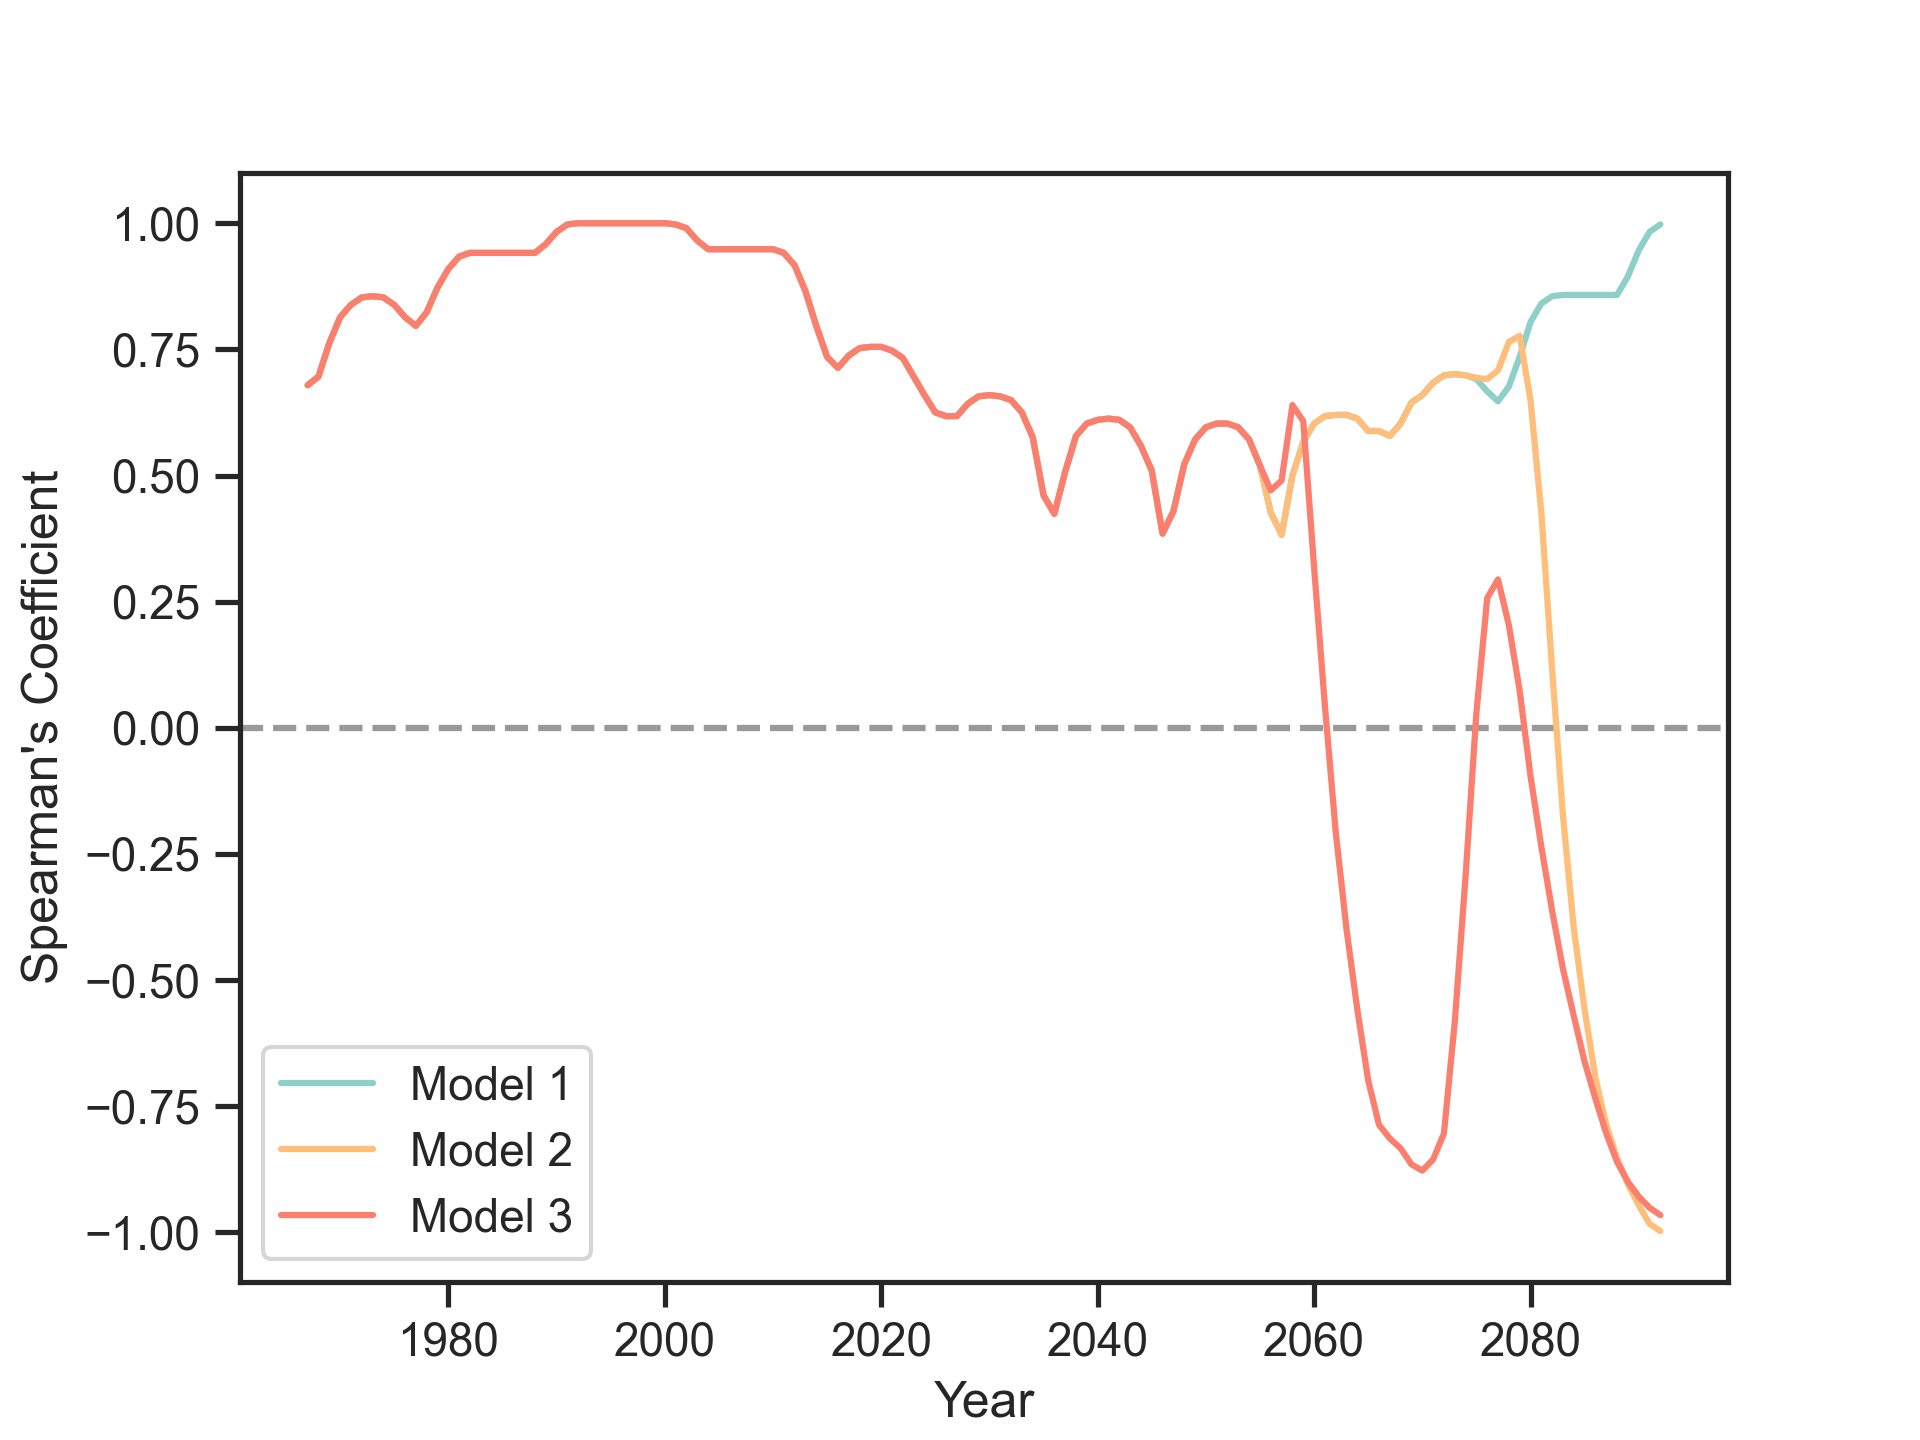
\includegraphics[width = 0.7\textwidth]{fig/2b.png}
    \caption{Curves of partial Spearman's coefficient given by three models prediciting \ce{CO2} concentration}
    \label{m5:fig}
\end{figure}

As we see from the Figure, the three curves are all overlapped by each other before 2050. Yet in 2060 and 2080 respectively, curves of model 3 and model 2 begin to fall dramatically. This shows that after 2060, temperature and \ce{CO2} concentration(predicted by model 2 \& 3) no longer have similar trends. This fact thereby convinces us that our model predicting land-ocean temperature will be no longer accurate after 2060. 

\section{Model Comparison and Evaluation}

\begin{figure}[hbt]
    \centering
    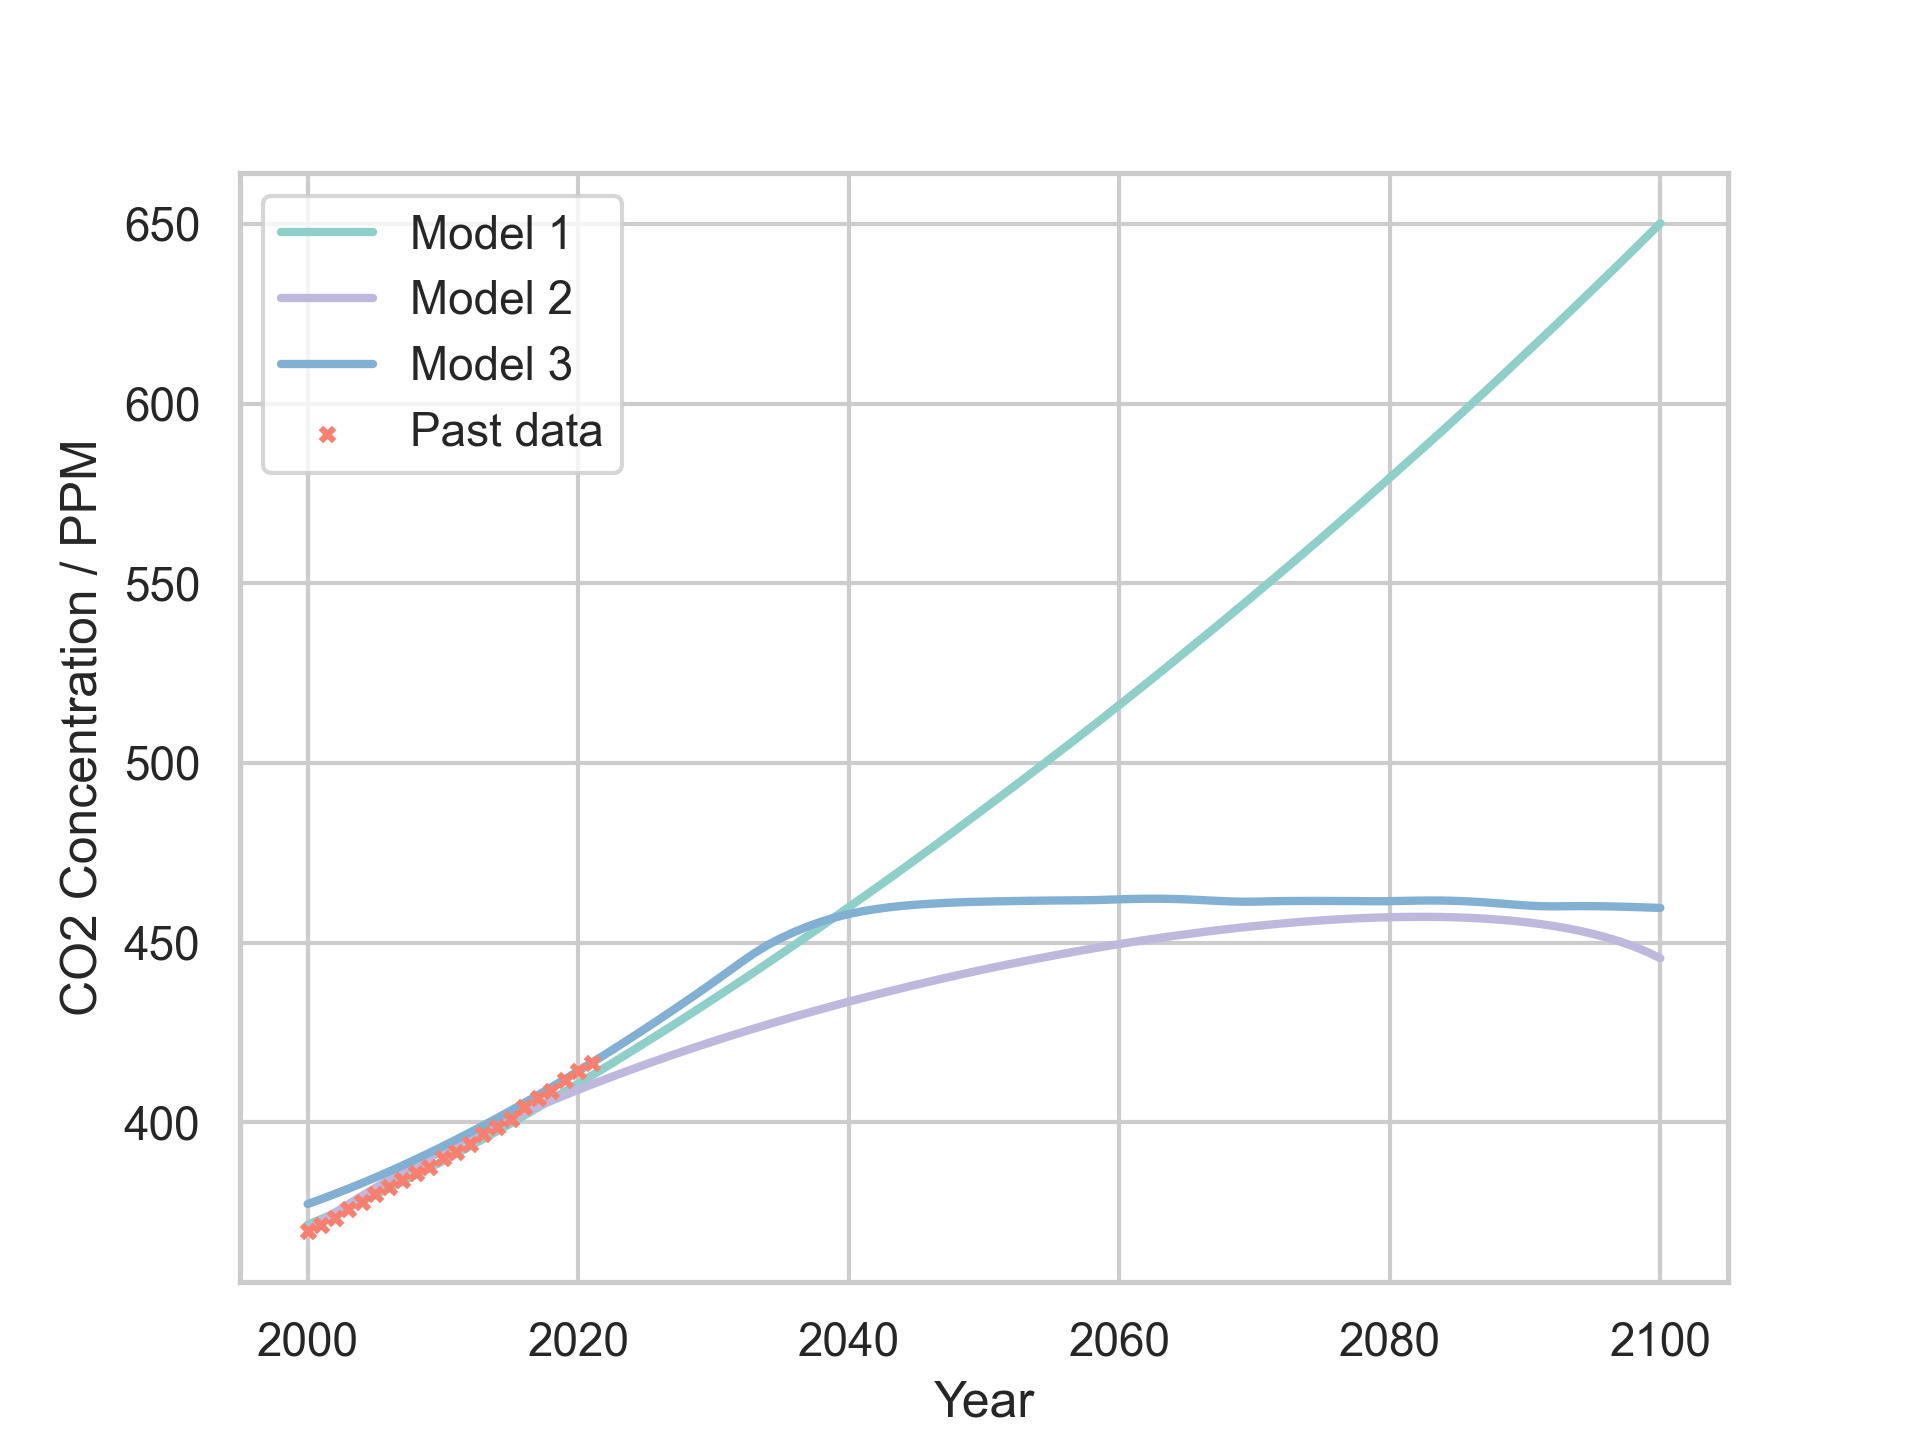
\includegraphics[width = 0.7\textwidth]{fig/General Projections.png}
    \caption{\ce{CO2} concentration prediction made by model $1\sim 3$}
    \label{general}
\end{figure}

We see in the Figure \ref{general} that Model 2 \& 3 give similar predictions, while projection values of Model 1 are much higher. Yet, all of the three models' predictions conclude that CO2 concentration will not reach as high as 685 PPM in 2050, not even in 2100. In fact, Model 1 predicted that CO2 concentration will go above 685 PPM in 2115, but the model will probably be no longer accurate after going through such long time.

To strengthen certain outstanding characteristics in each model, other aspects are sacrificed to reach inter-model balance. Among the models presented, we reckon Model 2 as the most accurate projection and Model 1 as the least realistic before year 2100. Model 1 has utilized all factors to give the prediction, but the predicting methods it adapts is not optimized for specific problem. Model 3 has considered the retroaction effect that CO2 exerts on humans, yet the feedback functions are artificially designed, which cannot be supported by the data. Model 2, adapting stepwise regression and borrowing STIRPAT equation from environmental science study, reasonably estimated the relation between major factors and CO2 concentration. The model gave a convincing prediction that CO2 concentration will hit a climax of 456 PPM in around 2085 and later fall back.

\section{Strengths and Weaknesses}

\subsection*{Strengths}

Model 1 is developed as all ten factors contribute to the eventual projection in different weights. This highly resembles the often situation in reality, where multiple factors decide the final result in minor proportions, instead of a few major ones determining every aspect.

In order to keep the models' flexibility factors changes, Model 2 embodied the original trends in determining factors when predicting by simplifying trends in selected factors directly form a compound algorithm. While it provides more flexible insights by simplifying the attribution of weight between factors, the form of exponential function also decides that the changing rate of factors and the independent factor $c$ beer a linear relationship, which is a more realistic way for variables to change.

By designing feedback functions, Model 3 clearly shows the influence of efforts to reduce carbon emissions taken into account. By focusing on the amount of \ce{CO2} emission -- the derivative of \ce{CO2} concentration with respect to time, instead of \ce{CO2} concentration itself, Model 3 is intuitively more reliable that other 2 models.

In model 4, we applied Lowess smoothing to rule out the noises and reflect the real trend of data. we artificially extract the vibrating pattern of land-ocean temperature, which is more accurate than that directly generated by linear regression models. In model 5, we adapted an innovative partial estimating strategy to predict future relation between temperature and \ce{CO2} concentration. 

\subsection*{Weaknesses}

We used all ten variables for the prediction, resulting in a problem that the more factors are, the bigger the possibility that intense changes occur after sudden disruptions. Thus, it becomes harder to avoid unreasonable bothers and to maintain the result within a reasonable interval, making the algorithm more fragile to sudden changes or long-term projections. In this case, it goes the opposite way from the other two projections and failed to foresee the positive changes in basic factors supporting the projection.

In model 3, we designed the feedback function artificially and there's nothing to support our design. Thereby, the effectiveness of the model relies heavily on our design. Also, the model predicts that \ce{CO2} concentration will maintain as high as 460 PPM, which seems not reasonable.

In model 4, we assume that solar activities affect the periodical pattern of temperature. Although the temperature curve fitted the data well, this assumption is not supported by the conclusion made by Grey Analysis in model 5.

\section{Conclusion}

To offer our own insight into the controversy, prior to the beginning of data selection, we set a clear direction: to model \ce{CO2} concentration and to describe its connection to temperature with multiple methods. Firstly, upon reflecting on previous papers, we selected ten factors that contain the widest range of emission sources. Through regression models and the reliable data provided by UN, we simulated the 10 factors' changes throughout the century. 

Before solving Problem 1, we first pointed out that the sharp increase in 2004 is not major to the largest 10-year average increase up of the 2000s according to the information officially admitted and confirmed accurate. Firstly, with PCA we reduced the 10 variables to 3. And with the following Multivariate Regression, we managed to yield the weight of each original factor. In model 2, we took on Stepwise Regression to select three factors bearing the most irreplaceability and related them with \ce{CO2} levels through STIRAPT equation. In the third model, we employed Differential Equation to express artificial feedbacks to the changes, in which ODE was applied to a function of two hand-picked factors, so as to compute the concentration around which human reacts with urgency. Three versions of the relationship were thus created. Accordingly, \ce{CO2} levels will not reach 685 before 2050 in any curve and the 2100 \ce{CO2} concentration is expected to range from 446 to 650 PPM, the former possessing larger possibility.

We began our solution of Problem 2 with the smoothening of the historical temperature curve through Lowess Smoothing. Due to its similarity to the figure, a quadratic function acts as the base of the projection. After amending the curve with three sine functions to restore the periodicity of original data, we concluded that average land-ocean will have risen 1.25$^\circ$C by 2028, 1.50$^\circ$C by 2037 and 2.0$^\circ$C by 2056. Then, we extended our vision to involve major contributors to the global warming. Factors other than \ce{CO2} include \ce{CH4}, \ce{N2O} and solar radiation. We applied GRG to compare the extent to which each factor is connected to changes in temperature. To further determine the influence of \ce{CO2} to global temperature by quantities, we used Spearman's coefficient and managed to express their singular connection. It turned out that \ce{CO2} is indeed responsible for the majority of global rising, as it ranked the highest in GRG proportion at 0.8 and related with temperature to the same extent using all three models in Problem 1. However, the Spearman's coefficient goes in separate trends after 2060, indicating the model's loss of accuracy starting from 2060.

\begin{thebibliography}{99}
    \bibitem{ref1} UN Department of Economic and Social Affairs. (2022, July). Methodology of the United Nations population estimates and projections. [Internet] https://population.un.org/wpp/Publications/Files/WPP2022\_Methodology.pdf
    \bibitem{ref450} Organisation for Economic Co-Operations and Development. (2012). The OECD environmental outlook to 2050. [Internet]
    https://www.oecd.org/env/cc/Outlook\%20to\%202050\_Climate\%20Change\%20Chapter\_HIGLIGHTS-FINA-8pager-UPDATED\%20NOV2012.pdf

    \bibitem{ref3} National Oceanographic and Atmospheric Administration. NOAA Earth System Research Laboratory. (2022, October). Trends in atmospheric carbon dioxide [Internet]. https://gml.noaa.gov/ccgg/trends/data.html

    \bibitem{ref5} NASA-JPL/Caltech. (2020). Graphic: Temperature vs Solar Activity. [Internet] https://climate.nasa.gov/climate\_resources/189/graphic-temperature-vs-solar-activity/

    \bibitem{STI} Richard York and Eugene A Rosa and Thomas Dietz. (2003). STIRPAdT, IPAT and ImPACT: analytic tools for unpacking the driving forces of environmental impacts. \textit{Ecological Economics}, 46, 351-365
\end{thebibliography}

\end{document}